\documentclass[11pt]{article}

\usepackage[margin=1in]{geometry}
\usepackage[T1]{fontenc}
\usepackage[utf8]{inputenc}
\usepackage{lmodern}
\usepackage{microtype}
\usepackage{amsmath,amssymb,amsthm,mathtools}
\usepackage{booktabs}
\usepackage{enumitem}
\usepackage{tikz}
\usetikzlibrary{arrows.meta,decorations.pathreplacing,calc}
\usepackage[dvipsnames]{xcolor}
\usepackage[colorlinks=true,linkcolor=MidnightBlue,citecolor=MidnightBlue,urlcolor=MidnightBlue]{hyperref}

\newtheorem{theorem}{Theorem}[section]
\newtheorem{lemma}[theorem]{Lemma}
\newtheorem{proposition}[theorem]{Proposition}
\newtheorem{corollary}[theorem]{Corollary}
\theoremstyle{definition}
\newtheorem{definition}[theorem]{Definition}
\newtheorem*{definition*}{Definition}
\theoremstyle{remark}
\newtheorem{remark}[theorem]{Remark}
\usepackage{comment}
\usepackage{listings}
\usepackage{upquote}

\lstdefinelanguage{Lean4}{
  morekeywords=[1]{import,open,scoped,noncomputable,def,structure,where,theorem,lemma,by,let,if,then,else,fun,simp,only,max},
  morekeywords=[2]{Prop,Type},
  morekeywords=[3]{sorry},
  sensitive=true,
  morecomment=[l]{--},
  morecomment=[s]{/-}{-/},
  morestring=[b]",
}

\lstdefinestyle{leanstyle}{
  language=Lean4,
  basicstyle=\fontsize{7.4}{7.85}\selectfont\ttfamily,
  keywordstyle=[1]\color{MidnightBlue}\bfseries,
  keywordstyle=[2]\color{MidnightBlue!80!black},
  keywordstyle=[3]\color{BrickRed}\bfseries,
  commentstyle=\color{gray!80!black}\slshape,
  numbers=left,
  numberstyle=\tiny\color{gray!85!black},
  numbersep=8pt,
  frame=single,
  framesep=4pt,
  xleftmargin=18pt,
  xrightmargin=4pt,
  rulecolor=\color{gray!40},
  backgroundcolor=\color{gray!4},
  columns=fullflexible,
  keepspaces=true,
  upquote=true,
  showstringspaces=false,
  aboveskip=0pt,
  belowskip=0pt,
  literate=
    {ℝ≥0∞}{{$\mathbb{R}_{\ge 0}^\infty$}}4
    {×}{{$\times$}}1
    {β}{{$\beta$}}1
    {₀}{{$_0$}}1
    {₁}{{$_1$}}1
    {₂}{{$_2$}}1
    {₊}{{$_+$}}1
    {ℕ}{{$\mathbb{N}$}}1
    {ℝ}{{$\mathbb{R}$}}1
    {→}{{$\;\to\;$}}1
    {∀}{{$\forall\,$}}1
    {∃}{{$\exists\,$}}1
    {∈}{{$\in$}}1
    {∑}{{\scalebox{0.72}{$\textstyle\sum$}}}1
    {∞}{{$\infty$}}1
    {∧}{{$\land$}}1
    {∨}{{$\lor$}}1
    {≠}{{$\ne$}}1
    {≤}{{$\le$}}1
    {≥}{{$\ge$}}1
    {⊕}{{$\oplus$}}1
    {⌈}{{\smash{$\lceil$}}}1
    {⌉}{{\smash{$\rceil$}}}1
    {⟨}{{\smash{$\langle$}}}1
    {⟩}{{\smash{$\rangle$}}}1
    {⨅}{{\raisebox{-0.12ex}{\scalebox{1.15}{$\sqcap$}}}}1,
}

% Comments for coauthors: write \todo{...} (or \TODO{...}) anywhere in the text; it is typeset in red.
\newcommand{\todo}[1]{\textcolor{red}{[TODO: #1]}}
\newcommand{\TODO}[1]{\todo{#1}}
\newcommand{\enote}[1]{\footnote{\textcolor{red}{Erik: }#1}}

\newcommand{\R}{\mathbb{R}}
\newcommand{\N}{\mathbb{N}}
\newcommand{\dH}{\mathrm{d}_H}
\newcommand{\dP}{\mathrm{d}_P}
\newcommand{\Ham}{\mathrm{Ham}}
\newcommand{\dHam}{\mathrm{d}_{\Ham}}
\newcommand{\Ber}{\operatorname{Ber}}
\newcommand{\Bin}{\operatorname{Bin}}
\newcommand{\diam}{\operatorname{diam}}
\title{\textbf{Constant-Stretch High-Dimensional Spanners\\Require Super-Linear Size}}
\author{
  Rajesh Jayaram\\[-2pt] {\small Google Research} \and
  Vahab Mirrokni\\[-2pt] {\small Google Research} \and
  Erik Waingarten\\[-2pt] {\small University of Pennsylvania} \and
  David P. Woodruff\\[-2pt] {\small Google Research \& CMU} \and
  Goran Zuzic\\[-2pt] {\small Google Research}
}

\date{November 2026}

\begin{document}
\maketitle
\begin{abstract}
Since the work of Indyk and Motwani (1998), algorithms for high-dimensional geometric problems have avoided the curse of dimensionality by making two concessions: they approximate within a constant factor $C$, and they pay a polynomial overhead, using time or space $n^{1 + \rho}$, where $\rho = \rho(C) > 0$ tends to $0$ as $C$ grows. Whether the overhead is necessary is open: for basic problems such as bichromatic closest pair, it is not known whether \emph{some} constant-factor approximation can be computed in time $n^{1 + o(1)}$.

We show that the overhead is necessary for spanners. A $C$-spanner of a point set is a weighted graph on the points whose shortest-path distances approximate all pairwise distances within a factor $C$, the \emph{stretch}. In high-dimensional Euclidean space, locality-sensitive hashing gives $C$-spanners with $\tilde{O}(n^{1 + O(1/C^2)})$ edges for large constant $C$, and it was open whether $n^{1 + o(1)}$ edges suffice for some constant $C$ (Har-Peled, Indyk, and Sidiropoulos, 2013; Krauthgamer and Petruschka, 2026). They do not: for every $p \in [1, \infty)$ and every constant $C \ge 1$, there are arbitrarily large $n$-point subsets of $\{0, 1\}^{O(\log n)}$ all of whose $C$-spanners in the $\ell_p$ norm have
\[
\Omega\bigl(n^{1 + c}\bigr) \ \text{edges}, \qquad \text{where } c = c(C, p) = 2^{-O(C^{3p}\log(C^p + 1))} > 0.
\]
Here $1/c$ is singly exponential in a polynomial of $C$; in particular, $c = 2^{-O(C^3 \log(C + 1))}$ in $\ell_1$ and $c = 2^{-O(C^6 \log(C + 1))}$ in $\ell_2$. Earlier lower bounds of the form $n^{1 + \Omega(1)}$ applied only to stretch below $2$, or to spanners in which every pair of points is joined by a path with at most two edges. Ours allows arbitrary paths, and even additional Steiner vertices that are not points of the space.

For general metrics, the hard instances for spanners are graphs of large girth, whose metrics are incompressible: no representation of any kind can be much smaller than the graph itself. Euclidean metrics can be compressed, to $O(\log n)$ numbers per point by the Johnson--Lindenstrauss lemma; yet, by our theorem, no undirected graph of near-linear size represents them within a fixed constant factor. The hard point sets are sampled from the solution sets of random constraint satisfaction problems. All main results have been formally verified in Lean~4 (\href{https://github.com/goranzuzic/high-dimensional-steiner-spanners}{\texttt{github.com/\allowbreak goranzuzic/\allowbreak high-\allowbreak dimensional-\allowbreak steiner-\allowbreak spanners}}).
\end{abstract}


\tableofcontents

% ============================================================================
\section{Introduction}
\label{sec:intro}
% ============================================================================

Many geometric computational problems on $n$ points in $\R^d$, such as nearest-neighbor search, closest pair, minimum spanning tree, and clustering, can be solved exactly or within a factor $1 + \varepsilon$ in near-linear time when the dimension $d$ is a constant. The running times grow exponentially with $d$, however, and for $d \gg \log n$ these algorithms are often no faster than brute force. In their seminal work, Indyk and Motwani~\cite{indyk1998approximate} proposed a way around this \emph{curse of dimensionality} for the approximate nearest neighbor search problem based on randomized space partitions---since then, randomized space partitions have become a standard toolkit in high-dimensional geometric problems. 

The effective use of randomized space partitions, however, typically requires both settling for a large constant approximation factor $C > 1$ and incurring a polynomial overhead of the form $n^{1 + \rho(C)}$ rather than $n^{1 + o(1)}$, where $\rho(C) > 0$ shrinks as $C$ grows. For instance, locality-sensitive hashing (LSH) achieves $\rho = 1/C$ in $\ell_1$ and $\rho = 1/C^2 + o(1)$ in $\ell_2$ for nearest-neighbor search~\cite{indyk1998approximate,andoni2008near} (further improved via data-dependent hashing~\cite{andoni2015optimal}), and the same trade-off appears in the best known algorithms for closest pair~\cite{indyk1998approximate,harpeled2012approximate}, minimum spanning tree construction~\cite{harpeled2012approximate,harpeled2013euclidean}, and agglomerative clustering~\cite{borodin1999subquadratic,harpeled2012approximate}. Almost three decades after~\cite{indyk1998approximate}, it remains open whether this polynomial overhead is inherent---for example, whether \emph{any} constant $C$ admits an $n^{1 + o(1)}$-time algorithm for $C$-approximate bichromatic closest pair in $\R^{O(\log n)}$, or whether, as Rubinstein~\cite{rubinstein2018hardness} asks, near-linear-time algorithms can be ruled out for every constant approximation factor. Existing lower bounds on $\rho(C)$ apply only to LSH~\cite{motwani2007lower,odonnell2014optimal} or restricted data structures~\cite{panigrahy2010lower,andoni2017optimal}, while the conditional lower bounds of~\cite{rubinstein2018hardness} hold only for $(1 + \varepsilon)$-approximations and face a triangle-inequality barrier starting at factor $3$.

We study this question for \emph{spanners}. A $C$-spanner of a finite metric space $(P, \dP)$ is a weighted graph on $P$ whose shortest-path distances are at least the distances in $P$ and exceed them by at most a factor $C$, called the \emph{stretch} (Definition~\ref{def:spanner}). A spanner with few edges is a sparse substitute for the metric: graph algorithms for minimum spanning trees~\cite{harpeled2013euclidean,filtser2022light}, Steiner trees~\cite{kou1981fast,mehlhorn1988faster}, and approximate distance oracles~\cite{thorup2005approximate} can be run on it instead of on all $\binom{n}{2}$ pairs of points, at the cost of a factor $C$ in the approximation. Har-Peled, Indyk, and Sidiropoulos~\cite{harpeled2013euclidean} showed that LSH yields, for every $n$-point subset of $\ell_2$ and every sufficiently large $C$, a $C$-spanner with $\tilde{O}(n^{1 + O(1/C^2)})$ edges, where $\tilde{O}$ hides polylogarithmic factors; more generally, $C$-spanners with $\tilde{O}\bigl(n^{1 + O_p(1/C^{\min(p, 2)})}\bigr)$ edges exist in every $\ell_p$ space~\cite{althofer1993sparse,filtser2022light,krauthgamer2025lipschitz,krauthgamer2025power}, matching the general-metric $(2k - 1)$-spanner bound $O(n^{1 + 1/k})$~\cite{althofer1993sparse} when $p = 1$. Spanners of this kind are also used in practice, to build very large similarity graphs for clustering and graph learning~\cite{carey2022stars}. Whether the polynomial overhead can be avoided was open. Krauthgamer and Petruschka~\cite[Question~1.1]{krauthgamer2026towards} recently singled out the following question as the main focus of their work on high-dimensional spanners:
\begin{quote}
\emph{Does every $n$-point subset of high-dimensional Euclidean space admit an $O(1)$-spanner with $n^{1 + o(1)}$ edges?}
\end{quote}
As they point out, even less was known for $\ell_1$: for stretch greater than $2$ there was no upper bound better than the one for general metrics, and the only lower bounds of the form $n^{1 + \Omega(1)}$ were for spanners in which every pair of points is joined by a path with at most two edges.

We answer this question in the negative, for every constant stretch $C$ and every $\ell_p$ norm with $1 \le p < \infty$: there are $n$-point subsets of $\{0, 1\}^{O(\log n)}$ on which every $C$-spanner has $\Omega(n^{1 + c})$ edges, where $c = 2^{-O(C^{3p}\log(C^p + 1))} > 0$ (Theorem~\ref{thm:geometric}). The lower bound holds in a much more permissive model, in which the graph may contain an arbitrary number of additional \emph{Steiner} vertices, joined to the points and to each other by edges of arbitrary non-negative weights; the only requirement is that the shortest-path distances between the original points be correct up to the factor $C$ (Theorem~\ref{thm:main}). Following~\cite{andoni2023subquadratic}, we call such graphs \emph{non-metric Steiner spanners}. Steiner vertices are useful: directed non-metric Steiner spanners are the basis of subquadratic approximation algorithms for transportation problems~\cite{andoni2023subquadratic,jayaram2026near}. Non-metric Steiner spanners also capture every covering of the points by clusters or hash buckets in which each pair of points shares a bucket of diameter at most $C$ times their distance: add one Steiner vertex per bucket (Proposition~\ref{prop:bucketing}). For such two-level coverings a lower bound was already known~\cite{krauthgamer2026towards}; the general model also allows, for instance, hierarchies of buckets, and paths with any number of edges.

Consequently, no algorithm that first builds an undirected graph whose shortest paths approximate all pairwise distances within a constant factor, with or without Steiner vertices, can run in time $n^{1 + o(1)}$: on some inputs the graph alone has $n^{1 + \Omega(1)}$ edges. This is evidence of a new kind that the polynomial overhead is necessary. For large approximation factors, unconditional lower bounds were previously known only for hashing schemes~\cite{motwani2007lower,odonnell2014optimal}, for restricted classes of data structures~\cite{panigrahy2010lower,andoni2017optimal}, and for spanners in which every pair of points is joined by a path with at most two edges~\cite{harpeled2013euclidean,krauthgamer2026towards}. Our theorem says nothing about algorithms that do not go through a spanner; whether such an algorithm can run in near-linear time remains open (Section~\ref{sec:open}).

The theorem also separates two ways of storing a metric. For general metrics, the hard instances for spanners are graphs of large girth, and a counting argument shows that their metrics are incompressible: no representation of any kind can be much smaller than the graph itself, so they have neither a small distance oracle nor a low-distortion embedding into a low-dimensional normed space~\cite{thorup2005approximate,matousek1996distortion}. Euclidean metrics can be compressed: by the Johnson--Lindenstrauss lemma, $O(\log n)$ numbers per point determine all distances within a factor $1 + \varepsilon$. For every constant $C$, there are point sets that are described exactly by $O(n \log n)$ bits, and yet no undirected graph with $n^{1 + o(1)}$ edges represents their distances within the factor $C$. We discuss this in Section~\ref{subsec:background}.

\subsection{Our Results}
\label{subsec:results}

\begin{definition}[Spanners, Steiner Spanners, and Aspect Ratio]
\label{def:spanner}
Given a finite metric space $(P, \dP)$ on $n = |P| \ge 2$ input points (called \emph{terminals}) and a target \emph{stretch} $C \ge 1$, a $C$-spanner is an undirected weighted graph whose shortest paths never underestimate distances between terminals and overestimate them by at most a factor of $C$.

Formally, let $H = (P \sqcup S, E, w)$ be a finite undirected simple graph on the terminals $P$ together with a finite set $S$ of auxiliary \emph{Steiner vertices} ($P \cap S = \emptyset$), equipped with non-negative edge weights $w : E \to \R_{\ge 0}$. Let $\dH(u, v) \in [0, \infty]$ denote the shortest-path distance between $u$ and $v$ in $H$ (with $\dH(u, v) = \infty$ if $u$ and $v$ lie in different connected components). Depending on which auxiliary vertices and edge weights are permitted, we distinguish the following notions (Figure~\ref{fig:spanner-models}):
\begin{itemize}[leftmargin=2em,nosep,topsep=4pt,itemsep=3pt]
  \item \textbf{Undirected non-metric Steiner $C$-spanner} (hereafter simply \textbf{Steiner $C$-spanner}): $S$ may be any finite set and $w : E \to \R_{\ge 0}$ may assign arbitrary non-negative weights, provided that
  \[
  \dP(x, y) \;\le\; \dH(x, y) \;\le\; C \cdot \dP(x, y) \qquad \text{for all } x, y \in P.
  \]
  \item \textbf{Metric Steiner $C$-spanner}: a Steiner $C$-spanner in which $P \sqcup S$ lies in an ambient metric space $(X, \mathrm{d}_X)$ extending $\dP$, and every edge carries its ambient metric distance $w(\{u, v\}) = \mathrm{d}_X(u, v)$.
  \item \textbf{Geometric $C$-spanner}: a Steiner $C$-spanner with no auxiliary vertices ($S = \emptyset$) in which every edge carries the exact terminal distance $w(\{x, y\}) = \dP(x, y)$.
  \item \textbf{$k$-hop $C$-spanner}: a spanner $H$ (in any of the models above) in which every pair of distinct terminals $x, y \in P$ is joined by a simple path in $H$ of at most $k$ edges and total weight at most $C \cdot \dP(x, y)$.
\end{itemize}
Finally, for a finite point set $P \subset \R^d$ ($|P| \ge 2$) and $p \in [1, \infty)$, its $\ell_p$ \emph{aspect ratio} is the ratio of its largest to smallest nonzero pairwise distance,
\[
\Delta_p(P) \;:=\; \frac{\max_{x \ne y \in P} \|x - y\|_p}{\min_{x \ne y \in P} \|x - y\|_p}.
\]
\end{definition}

\begin{figure}[ht]
\centering
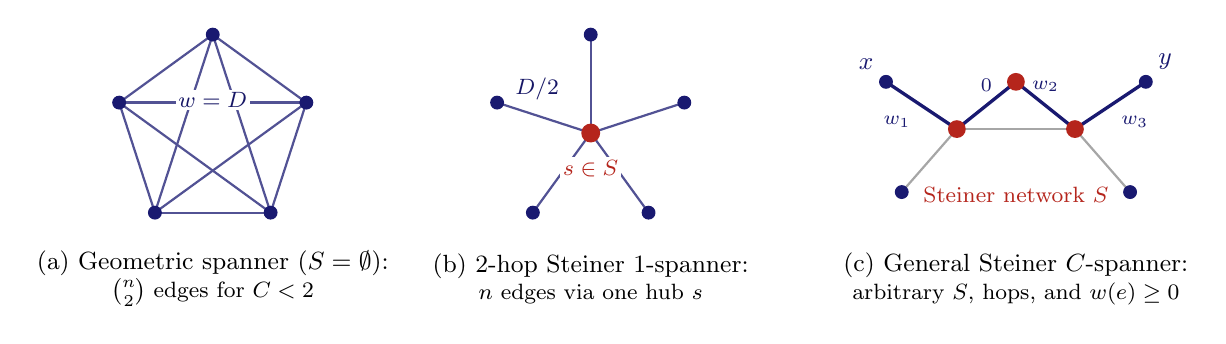
\begin{tikzpicture}[every node/.style={font=\small}]
  % === Panel (a): Geometric C-spanner ===
  \begin{scope}[shift={(0, 0)}]
    \foreach \i/\ang in {1/90, 2/162, 3/234, 4/306, 5/18} {
      \coordinate (a\i) at (\ang:1.25cm);
    }
    \foreach \i in {1,...,4} {
      \pgfmathtruncatemacro{\nexti}{\i + 1}
      \foreach \j in {\nexti,...,5} {
        \draw[thick, MidnightBlue!75] (a\i) -- (a\j);
      }
    }
    \foreach \i in {1,...,5} {
      \filldraw[MidnightBlue] (a\i) circle (2.3pt);
    }
    \node[MidnightBlue!90!black, fill=white, inner sep=1pt] at (0, 0.42) {\footnotesize $w = D$};
    \node[align=center] at (0, -1.85) {(a) Geometric spanner ($S = \emptyset$):\\[-1pt]{\footnotesize $\binom{n}{2}$ edges for $C < 2$}};
  \end{scope}

  % === Panel (b): 2-hop Steiner 1-spanner (star) ===
  \begin{scope}[shift={(4.8, 0)}]
    \coordinate (hub) at (0, 0);
    \foreach \i/\ang in {1/90, 2/162, 3/234, 4/306, 5/18} {
      \coordinate (b\i) at (\ang:1.25cm);
      \draw[thick, MidnightBlue!75] (hub) -- (b\i);
    }
    \foreach \i in {1,...,5} {
      \filldraw[MidnightBlue] (b\i) circle (2.3pt);
    }
    \draw[fill=white, very thick, BrickRed] (hub) circle (2.8pt);
    \node[BrickRed, fill=white, inner sep=1pt] at (0.0, -0.45) {\footnotesize $s \in S$};
    \node[MidnightBlue!90!black, fill=white, inner sep=1pt] at (-0.68, 0.56) {\footnotesize $D/2$};
    \node[align=center] at (0, -1.85) {(b) $2$-hop Steiner $1$-spanner:\\[-1pt]{\footnotesize $n$ edges via one hub $s$}};
  \end{scope}

  % === Panel (c): General non-metric Steiner C-spanner ===
  \begin{scope}[shift={(10.2, 0)}]
    \coordinate (x) at (-1.65, 0.65);
    \coordinate (z1) at (-1.45, -0.75);
    \coordinate (y) at (1.65, 0.65);
    \coordinate (z2) at (1.45, -0.75);
    \coordinate (s1) at (-0.75, 0.05);
    \coordinate (s2) at (0.0, 0.65);
    \coordinate (s3) at (0.75, 0.05);

    \draw[thick, gray!70] (z1) -- (s1);
    \draw[thick, gray!70] (s1) -- (s3);
    \draw[thick, gray!70] (z2) -- (s3);
    \draw[very thick, MidnightBlue] (x) -- node[below left=0pt, font=\scriptsize] {$w_1$} (s1)
      -- node[above=1pt, font=\scriptsize] {$0$} (s2)
      -- node[above=1pt, font=\scriptsize] {$w_2$} (s3)
      -- node[below right=0pt, font=\scriptsize] {$w_3$} (y);

    \filldraw[MidnightBlue] (x) circle (2.3pt) node[above left=1pt] {$x$};
    \filldraw[MidnightBlue] (y) circle (2.3pt) node[above right=1pt] {$y$};
    \filldraw[MidnightBlue] (z1) circle (2.3pt);
    \filldraw[MidnightBlue] (z2) circle (2.3pt);

    \draw[fill=white, very thick, BrickRed] (s1) circle (2.6pt);
    \draw[fill=white, very thick, BrickRed] (s2) circle (2.6pt);
    \draw[fill=white, very thick, BrickRed] (s3) circle (2.6pt);
    \node[BrickRed, fill=white, inner sep=1pt] at (0, -0.78) {\footnotesize Steiner network $S$};

    \node[align=center] at (0, -1.85) {(c) General Steiner $C$-spanner:\\[-1pt]{\footnotesize arbitrary $S$, hops, and $w(e) \ge 0$}};
  \end{scope}
\end{tikzpicture}
\caption{Spanner models in Definition~\ref{def:spanner} (solid blue circles: terminals in $P$; open red circles: Steiner vertices in $S$). On $n$ points at pairwise distance $D$, a geometric $C$-spanner with $C < 2$ requires all $\binom{n}{2}$ edges~(a), whereas a single Steiner hub with spoke weights $D/2$ achieves stretch $1$ in $n$ edges~(b). Theorem~\ref{thm:main} holds against arbitrary Steiner $C$-spanners~(c), where shortest paths may use any number of Steiner vertices and arbitrary weights $w(e) \ge 0$ (including $0$) subject only to $\dP(x, y) \le \dH(x, y) \le C \cdot \dP(x, y)$ on $P$.}
\label{fig:spanner-models}
\end{figure}

Throughout, all spanners in our results are undirected, $O_{C, p}(\cdot)$ and $\Theta_{C, p}(\cdot)$ hide constants that depend only on $C$ and $p$ (and similarly for other subscripts), and $\tilde{O}(\cdot)$ hides polylogarithmic factors.

Our main result is a lower bound for Steiner spanners. We first state its consequence for geometric spanners.

\begin{theorem}[Lower Bound for Geometric Spanners]
\label{thm:geometric}
Let $p \in [1, \infty)$ and $C \ge 1$. There exist constants $c = c(C, p) > 0$ and $c_0 = c_0(C, p) > 0$ such that for infinitely many $n$ there is an $n$-point set $P_n \subset \{0, 1\}^{d(n)}$, in dimension $d(n) = \Theta_{C, p}(\log n)$ and with aspect ratio $\Delta_p(P_n) = O_{C, p}(1)$, for which every geometric $C$-spanner of $(P_n, \|\cdot\|_p)$ has at least $c_0\, n^{1 + c}$ edges. Moreover, $c(C, p) = 2^{-O(C^{3p}\log(C^p + 1))}$ with an absolute implicit constant; in particular, $c(C, 1) = 2^{-O(C^3 \log(C + 1))}$ in $\ell_1$ and $c(C, 2) = 2^{-O(C^6 \log(C + 1))}$ in $\ell_2$.
\end{theorem}

Theorem~\ref{thm:geometric} is a special case of our main theorem, because a geometric spanner is a Steiner spanner without Steiner vertices.

\begin{theorem}[Main Theorem: Lower Bound for Steiner Spanners]
\label{thm:main}
Let $p \in [1, \infty)$ and $C \ge 1$ be reals, and set $C_1 := \max(3, \lceil C^p \rceil)$. There exist constants $c, c_0 > 0$, $0 < \beta_1 \le \beta_2$, and $A > 0$, all depending only on $C_1$, and infinitely many integers $n \ge 2$ such that for each of them there are an integer $d(n) \ge 1$ and an $n$-point set $P_n \subset \{0, 1\}^{d(n)}$ with
\[
\beta_1 \log_2 n \;\le\; d(n) \;\le\; \beta_2 \log_2 n \qquad \text{and} \qquad \Delta_p(P_n) \;\le\; A,
\]
for which every Steiner $C$-spanner $H = (P_n \sqcup S, E, w)$ of $(P_n, \|\cdot\|_p)$ satisfies
\[
|E| \;\ge\; c_0 \cdot n^{1 + c}.
\]
Moreover, $c = 2^{-O(C_1^3 \log C_1)} = 2^{-O(C^{3p}\log(C^p + 1))}$, with absolute implicit constants.
\end{theorem}

\paragraph{How far from optimal?}
Theorem~\ref{thm:main} leaves two gaps. For constant stretch $C$, our exponent $c = 2^{-O(C^6 \log(C + 1))}$ in $\ell_2$ is far from the exponent $O(1/C^2)$ of the upper bound~\cite{harpeled2013euclidean}. And it is not known how large the stretch must be for spanners with $n \cdot \mathrm{polylog}(n)$ edges: by Theorem~\ref{thm:main} it cannot be bounded by a constant, while $O(\sqrt{\log n})$ suffices in $\ell_2$~\cite{harpeled2013euclidean}. With $n^{1 + o(1)}$ edges, on the other hand, every stretch that tends to infinity can be achieved, already in general metric spaces~\cite{althofer1993sparse}; in this sense the assumption of constant stretch in Theorem~\ref{thm:main} cannot be weakened. See Section~\ref{sec:open}.

\paragraph{The hard point sets.}
The sets $P_n$ are subsets of the Boolean hypercube in dimension $\Theta_{C, p}(\log n)$, with bounded aspect ratio. Logarithmic dimension is the least possible: since $(\R^d, \|\cdot\|_p)$ has doubling dimension $O(d)$, every $n$-point set in dimension $d = o(\log n)$ has a $(1 + \varepsilon)$-spanner with $\varepsilon^{-O(d)} n = n^{1 + o(1)}$ edges~\cite{harpeled2006fast} (see also~\cite{arya1995euclidean,le2019truly} for the Euclidean case). Bounded aspect ratio means that the lower bound arises at a single distance scale rather than from an interplay of many scales. The sets are obtained by the probabilistic method. While the exponent $c = 2^{-O(C_1^3 \log C_1)}$ is singly exponential in a polynomial of $C_1$, the constants $\beta_1, \beta_2$ in the dimension are doubly exponential in a polynomial of $C_1$.

\paragraph{Other norms.}
Theorem~\ref{thm:main} applies to every $p \in [1, \infty)$, with an exponent that deteriorates as $p$ grows. For $p > 2$ this can be avoided: embedding our hard instances for $\ell_2$ into $\ell_p$ via Dvoretzky's theorem~\cite{figiel1977dimension} gives an exponent that does not depend on $p$, at the price of non-Boolean coordinates and polylogarithmic dimension (Corollary~\ref{cor:lp-dvoretzky}, proved in Section~\ref{subsec:master-proof}). For comparison, the known upper bounds for $p > 2$ have exponent $O_p(1/C^2)$~\cite{krauthgamer2025lipschitz,krauthgamer2025power}. The case $p = \infty$ was known: every $n$-point metric space embeds isometrically into $\ell_\infty^n$, so the lower bounds for general metrics apply.

\begin{corollary}[$p$-Independent Exponent for $p > 2$]
\label{cor:lp-dvoretzky}
Fix any real $p \in (2, \infty)$ and any constant $C \ge 1$. For infinitely many $n$, there is an $n$-point set $P_n \subset \R^{d(n)}$ in dimension $d(n) = \Theta_{C, p}\bigl((\log n)^{p/2}\bigr)$ with aspect ratio $\Delta_p(P_n) = O_C(1)$ on which every Steiner $C$-spanner (and hence every geometric $C$-spanner) of $(P_n, \|\cdot\|_p)$ has at least $c_0(C)\,n^{1 + c(C)}$ edges, where $c(C) = 2^{-O(C^6 \log(C + 1))} > 0$ and $c_0(C) > 0$ depend only on $C$.
\end{corollary}

\subsection{Sparse Graphs versus Compact Descriptions}
\label{subsec:background}

How sparse can a graph be if its shortest-path metric is to approximate a given $n$-point metric within a constant factor? For general metrics the answer has long been understood. Every $n$-point metric space has a $(2k - 1)$-spanner with $O(n^{1 + 1/k})$ edges~\cite{althofer1993sparse}. This is optimal if the girth conjecture of Erd\H{o}s~\cite{erdos1964extremal} holds. Unconditionally, the high-girth graphs obtained by the probabilistic method~\cite{erdos1959graph} show that $n^{1 + \Omega(1/C)}$ edges are necessary for stretch $C$, even when arbitrary Steiner vertices are allowed~\cite{althofer1993sparse,rabinovich1998lower}.

These lower bounds reflect \emph{incompressibility}. A graph with $m$ edges and large girth has $2^m$ subgraphs, and the shortest-path metrics of any two of them differ by a large factor on some pair of vertices; hence every data structure that approximates all of these metrics within a smaller factor must use at least $m$ bits. For general metrics, therefore, not only spanners but all compact representations are subject to the same kind of bound, for instance approximate distance oracles~\cite{thorup2005approximate} and low-distortion embeddings into low-dimensional normed spaces~\cite{matousek1996distortion}.

High-dimensional Euclidean metrics are different, because they \emph{are} compressible. By the Johnson--Lindenstrauss lemma~\cite{johnson1984extensions}, every $n$-point subset of $\ell_2$ can be mapped into $O(\varepsilon^{-2} \log n)$ dimensions while changing all distances by at most a factor $1 + \varepsilon$, so that $O(\log n)$ numbers per point describe the whole metric up to a factor $1 + \varepsilon$; analogous sketches exist in $\ell_p$ for every $1 \le p \le 2$~\cite{indyk2006stable}. No counting argument can therefore give a lower bound of the form $n^{1 + \Omega(1)}$ for spanners in these spaces, and the question is whether a compact description of the metric can always be organized as a sparse \emph{graph}. This is not implausible, especially when Steiner vertices are allowed. For example, $n$ equidistant points need $\binom{n}{2}$ edges in every geometric spanner of stretch below $2$, but they are represented exactly by a star with a single Steiner vertex and $n$ edges (Proposition~\ref{prop:simplex}).

Theorems~\ref{thm:geometric} and~\ref{thm:main} show that the answer is nevertheless negative. For every constant $C$, they provide point sets in $\{0, 1\}^{O(\log n)}$, which are described \emph{exactly} by $O(n \log n)$ bits and hence have an exact distance oracle of that size, whose metric cannot be approximated within the factor $C$ by any undirected weighted graph with $n^{1 + o(1)}$ edges. In this sense, shortest paths in a sparse undirected graph are a strictly weaker way of representing a high-dimensional $\ell_p$ metric than a short description, and the polynomial overhead of spanners reflects a limitation of shortest paths rather than of information.

\subsection{Previous Lower Bounds and Related Work}
\label{subsec:related}

Since counting arguments are not available, the known lower bounds for high-dimensional spanners use the geometry of specific point sets, and they apply only to stretch below $2$ or to restricted classes of spanners.

\paragraph{Stretch below $2$.}
A set of $n$ equidistant points requires $\binom{n}{2}$ edges in every geometric spanner of stretch below $2$. Andoni and Zhang~\cite{andoni2023subquadratic} showed that $n^{2 - o(1)}$ edges are necessary for stretch below $\sqrt{2}$ even for metric Steiner spanners in Euclidean space, and for stretch $1 + \varepsilon$ a lower bound of $\tilde{\Omega}(n^{2 - O(\varepsilon)})$ is known even for directed non-metric Steiner spanners~\cite{jayaram2026near}, and hence also for undirected ones. These bounds say nothing about larger stretch: $n$ equidistant points, for instance, have a geometric $2$-spanner with $n - 1$ edges (a star centered at one of the points), and with a single Steiner vertex they are represented exactly.

\paragraph{Two hops.}
For larger stretch, lower bounds were known only for \emph{$2$-hop} spanners, in which every pair of points must be joined by a path with at most two edges (hops) and weight at most $C$ times their distance. Har-Peled, Indyk, and Sidiropoulos~\cite{harpeled2013euclidean} proved that $2$-hop $C$-spanners of the hypercube $\{0, 1\}^d$ in $\ell_2$ need $n^{1 + \Omega(1/C^2)}$ edges, where $n = 2^d$, and Krauthgamer and Petruschka~\cite[Theorem~1.2 and Remark~3.2]{krauthgamer2026towards} gave a simpler proof, through a reduction to lower bounds for LSH~\cite{motwani2007lower}, that also covers non-metric Steiner vertices and all $\ell_p$ norms, with $n^{1 + \Omega(1/C^p)}$ edges. As soon as three hops are allowed, no such bound holds for the hypercube, which then has a spanner with constant stretch and $O(n \log \log n)$ edges~\cite[Theorem~A.1]{krauthgamer2026towards} (see also Proposition~\ref{prop:three-hop}(b)). In Section~\ref{sec:warmups} we show that this phenomenon is robust: in every sufficiently dense subset $P$ of the hypercube, all pairs at a given distance scale can be connected by three-hop paths of constant stretch, through Steiner vertices in the hypercube, using only $2|P|$ edges (Proposition~\ref{prop:three-hop}(a)). Hard instances inside the hypercube therefore cannot be dense subsets.

\paragraph{From bounded hops to general spanners.}
The paper~\cite{krauthgamer2026towards} also proves a hop-reduction theorem~\cite[Theorem~1.3]{krauthgamer2026towards}: if every subset $Y$ of an $n$-point metric space $X$ has a $t$-spanner with at most $\mu |Y|$ edges, then $X$ has an $O(t)$-hop $O(t)$-spanner with $O(n(\mu + \log n))$ edges. In contrapositive form, a sufficiently strong lower bound for $O(t)$-hop spanners of $X$ would imply a lower bound for spanners without a hop restriction on some subset of $X$. As the authors explain, the difficulty with this route is that their lower-bound technique does not extend beyond two hops, and that the hypercube itself has a $3$-hop spanner of constant stretch and near-linear size. Our proof does not pass through bounded-hop spanners. It handles paths of arbitrary length directly, on sparse, randomly constructed subsets of the hypercube, and it applies to Steiner spanners, a model in which the weight of a path does not bound its number of hops, because Steiner vertices can be joined by edges of weight zero.

\paragraph{Graphs of large girth.}
One might also hope to transfer the lower bound for general metrics by embedding the shortest-path metric of a graph $G$ of girth $g$ into $\ell_1$ or $\ell_2$. For the girth argument to survive at stretch $C$, the embedding must have distortion less than $(g - 1)/C$. However, the standard high-girth graphs with $n^{1 + \Omega(1/g)}$ edges are expanders with typical distances $\Omega(g)$, and by the Poincar\'e inequality of Linial, London, and Rabinovich~\cite{linial1995geometry} they require distortion $\Omega(g)$ in both $\ell_1$ and $\ell_2$. With the known constructions, this approach is therefore limited to stretch below an absolute constant. To go further one would need dense graphs of girth $g$ that embed into $\ell_1$ or $\ell_2$ with distortion $o(g)$. None are known. In $\ell_2$, for regular graphs their existence would contradict a conjecture of~\cite{linial1995geometry}, according to which every $k$-regular graph of girth $g$ with $k \ge 3$ requires Euclidean distortion $\Omega(g)$; a lower bound of $\Omega(\sqrt{g})$ was proved by Linial, Magen, and Naor~\cite{linial2002girth}. In $\ell_1$ there is no such obstacle: there are graphs of constant degree and arbitrarily large girth that embed into $\ell_1$ with uniformly bounded distortion~\cite{ostrovskii2012low}. These graphs, however, have only $O(n)$ edges.

\subsection{Technical Overview}
\label{subsec:intuition}

The proof has three steps. Step~1 replaces an arbitrary Steiner spanner by an unweighted graph on the points themselves, with no more edges, in which nearby points are joined by paths that stay nearby. Step~2 is a charging argument: such a graph has, up to a constant factor, at least as many edges as there are pairs of points at a certain distance, provided that every potential edge can be given a short list of the points whose paths it may carry. Step~3 constructs point sets with many such pairs for which these lists exist; they are random subsets of the solution set of a random constraint satisfaction problem.

\paragraph{The point sets.}
Fix $p \in [1, \infty)$ and $C \ge 1$, and let $C_1 := \max(3, \lceil C^p \rceil)$. Our point sets are codes $\mathcal{X} \subseteq [q]^N$, that is, sets of strings of length $N$ over an alphabet $[q] = \{1, \dots, q\}$ of constant size, placed in the hypercube by the \emph{one-hot embedding} $\iota : [q]^N \to \{0, 1\}^{N q}$, which replaces every symbol by its indicator vector. Two strings at Hamming distance $h$ are mapped to points at $\ell_p$-distance $(2h)^{1/p}$, for all $p$ simultaneously. Hence the $\ell_p$ metric on $\iota(\mathcal{X})$ is a constant multiple of a power of the Hamming metric on $\mathcal{X}$, and stretch $C$ in $\ell_p$ corresponds to stretch $C^p \le C_1$ in Hamming distance. The codes that we construct have length $N = O_{C_1}(r_*)$ and minimum distance at least $\frac{1}{2} r_*$ for a parameter $r_*$, so that all distances are within a constant factor of each other. They have many \emph{close pairs}, that is, pairs of codewords at Hamming distance exactly $r_*$: a code with $n$ codewords has $n^{1 + \Omega(1)}$ of them. The goal is to show that the number of edges of every Steiner spanner of $\iota(\mathcal{X})$ is at least a constant, depending only on $C_1$, times the number of close pairs.

\paragraph{Step 1: Removing Steiner vertices and weights.}
Let $H = (P \sqcup S, E, w)$ be a Steiner $C$-spanner of a finite metric space $(P, \dP)$, and fix a scale $r > 0$. A shortest path in $H$ between two terminals may pass through many Steiner vertices and may use edges of very small weight, so neither the number of hops nor the individual weights can be controlled. We nevertheless obtain a simple object on the terminals alone. Map every vertex $u$ of $H$ to a terminal $\pi(u) \in P$ that is nearest to $u$ in the shortest-path metric $\dH$, and replace every edge $\{u, v\}$ of $H$ by the pair $\{\pi(u), \pi(v)\}$, discarding it if $\pi(u) = \pi(v)$ or $\dP(\pi(u), \pi(v)) > C r$. The result is an unweighted graph $\widehat{G}$ on $P$ with at most $|E|$ edges. We claim that every pair $x, y \in P$ with $\dP(x, y) \le r$ is still connected in $\widehat{G}$, by a path that stays inside the ball of radius $C r$ around $x$. Indeed, let $x = v_0, v_1, \dots, v_k = y$ be a shortest path in $H$; its length is $\dH(x, y) \le C r$. Since $x$ and $y$ are terminals, the nearest terminal $\pi(v_i)$ satisfies $\dH(v_i, \pi(v_i)) \le \min\bigl(\dH(v_i, x), \dH(v_i, y)\bigr)$, and therefore
\[
\dH(x, \pi(v_i)) \;\le\; \dH(x, v_i) + \dH(v_i, y) \;=\; \dH(x, y) \;\le\; C r
\]
and
\begin{align*}
\dH(\pi(v_{i-1}), \pi(v_i)) &\;\le\; \dH(\pi(v_{i-1}), v_{i-1}) + w(\{v_{i-1}, v_i\}) + \dH(v_i, \pi(v_i)) \\
&\;\le\; \dH(x, v_{i-1}) + w(\{v_{i-1}, v_i\}) + \dH(v_i, y) \;=\; \dH(x, y) \;\le\; C r.
\end{align*}
Because $\dP \le \dH$ on $P$, the same bounds hold for $\dP$. So every $\pi(v_i)$ lies in the ball of radius $C r$ around $x$, and consecutive vertices $\pi(v_{i-1})$ and $\pi(v_i)$ are either equal or adjacent in $\widehat{G}$.

This argument loses nothing in the number of edges, however long the paths of $H$ are. What it gives up is all metric information beyond the scale $r$: the graph $\widehat{G}$ is merely an unweighted graph in which pairs at distance at most $r$ are connected \emph{locally}. This is why the argument does not conflict with the known lower bounds for Steiner point removal, where a minor on the terminals has to preserve all distances up to a small factor~\cite{chan2006steiner,chen2024lower}.

Applied to $P = \iota(\mathcal{X})$ at the scale of the close pairs, Step~1 reduces Theorem~\ref{thm:main} to a combinatorial statement about codes: for a suitable code $\mathcal{X}$, if $\widehat{G}$ is a graph on $\mathcal{X}$ with edges of Hamming length at most $C_1 r_*$ in which each close pair $(x, y)$ is joined by a path inside the Hamming ball of radius $C_1 r_*$ around $x$, then the number of edges of $\widehat{G}$ is at least a constant times the number of close pairs.

\paragraph{Step 2: A charging argument.}
Why should such a statement be true, and for which codes? For the full hypercube it is false. There, a near-linear number of edges suffices, because all close pairs can be routed along three-hop paths $x \to h(x) \to h(y) \to y$, where $h(x)$ and $h(y)$ are nearby codewords of a Hamming code~\cite{krauthgamer2026towards}, and each middle edge $\{h(x), h(y)\}$ serves very many pairs $(x, y)$. The same happens in every sufficiently dense subset of the hypercube (Section~\ref{sec:warmups}). A lower bound must therefore show that in $\mathcal{X}$ no edge can serve many close pairs, whatever the paths look like and wherever inside the ball they go.

To make this precise, suppose that we can attach to every ordered pair $(a, b)$ of nearby codewords a \emph{list} $\mathcal{L}(a, b) \subseteq \mathcal{X}$ of fewer than $K = O(C_1^2)$ codewords, defined in terms of the code alone and not of the graph. The list should be thought of as the set of origins $x$ that an edge $\{a, b\}$ is able to serve.

Given a close pair $(x, y)$ and a path $x = u_0, u_1, \dots, u_m = y$ in $\widehat{G}$ inside the ball around $x$, say that the $s$-th directed step $(u_{s-1}, u_s)$ of the path is \emph{marked} if $x = u_{s-1}$ or $x \in \mathcal{L}(u_{s-1}, u_s)$. The first step is marked. Let $(u_{s-1}, u_s)$ be the \emph{last} marked step and put $w_0 := u_s$. Since $x$ is one of at most $K$ codewords determined by the oriented edge $(u_{s-1}, u_s)$, at most $2 K |\widehat{E}|$ pairs $(x, w_0)$ arise in this way from all close pairs together. It remains to recover $y$ from $(x, w_0)$ up to $K$ possibilities. If $w_0 = y$, we are done. Otherwise the rest of the path leads from $w_0$ to $y$ without using a marked step. We will choose the lists so that this is possible only if $w_0$ is already \emph{aligned with} $y$, in the sense that $w_0$ differs from $x$ in more than a quarter of the $r_*$ coordinates in which $y$ differs from $x$. We will also make sure that, for every pair $(x, w_0)$, fewer than $K$ codewords $y$ at distance $r_*$ from $x$ have this property. Altogether, the number of close pairs is at most $K \cdot 2 K |\widehat{E}|$ (Theorem~\ref{thm:mod2-combinatorial}(a)).

\paragraph{Step 3: Random constraint satisfaction problems.}
It remains to find codes with many close pairs for which such lists exist. We obtain them from a random \emph{constraint satisfaction problem} with pairwise constraints (a $2$-CSP) on $N$ variables over the alphabet $[q]$, of a kind that is standard in the study of random CSPs~\cite{achlioptas2001random,molloy2003models}: for every pair of coordinates $u < v$, a random relation $R_{u, v} \subseteq [q] \times [q]$ contains each pair of symbols independently with a probability $p_{\mathrm{edge}} = 2^{-\sigma}$ slightly smaller than $1$ (in Section~\ref{sec:csp-cloud}, $\sigma$ is denoted $\sigma_{\mathrm{edge}}$). Let $\Omega(R) \subseteq [q]^N$ be the set of strings that satisfy all constraints. The code $\mathcal{X}$ is a random sample of $\Omega(R)$ from which a small number of atypical points have been deleted.

This distribution has the following feature. If $x \in \Omega(R)$ and $y$ differs from $x$ in a set $M$ of $m$ coordinates, then for $y$ to belong to $\Omega(R)$, roughly $m N$ further random constraints must hold, namely those that involve a coordinate of $M$. We choose $\sigma = \Theta_{C_1}(1/r_*)$ slightly above the threshold at which this cost balances the number of choices for $M$ and for the new symbols, so that each coordinate of $M$ carries a constant exponential penalty $2^{-\gamma_0}$, while the $\binom{m}{2}$ constraints between two coordinates of $M$ are counted once rather than twice and contribute a quadratic surplus $2^{\sigma \binom{m}{2}}$. Choosing $\gamma_0$ slightly below $\frac{1}{2}\sigma r_*$ ensures that a satisfying assignment still has $2^{\Theta_{C_1}(r_*)}$ expected neighbors at distance $r_*$, whereas any distance $m \le \frac{1}{2} r_*$ remains exponentially suppressed. Sampling the points of $\Omega(R)$ independently with a suitable probability $p_{\mathrm{keep}} = 2^{-\Theta_{C_1}(r_*)}$ therefore removes essentially all pairs at distance below $\frac{1}{2} r_*$, while a typical point keeps many close partners.

For larger $m$ up to $C_1 r_*$, the quadratic surplus $2^{\sigma \binom{m}{2}}$ overwhelms the linear penalty $2^{-\gamma_0 m}$, so a list defined as ``all codewords near $a$ and $b$'' would still be far too long. The way out is that a path in the spanner provides additional evidence about its origin. Suppose that $x$ is the origin of a path, that $(a, b)$ is an edge of the path, and that $z$ is any other vertex of the path; all four are satisfying assignments. If $u$ is a coordinate in which $z$ agrees with $x$ while $a$ and $b$ do not, and $v$ is a coordinate in which $z$ agrees with $a$ or $b$ but not with $x$, then, because $z$ satisfies the constraint on $(u, v)$, the relation $R_{u, v}$ contains the pair formed by the symbol of $x$ at $u$ and the symbol of $a$ or $b$ at $v$. We call this a \emph{hybrid constraint}. It is not implied by $x$, $a$, and $b$ being satisfying assignments: it is one more random constraint, which holds with probability $p_{\mathrm{edge}} = 2^{-\sigma}$. We define $\mathcal{L}(a, b)$ as the set of codewords $x$ near $a$ and $b$ for which enough hybrid constraints hold to reduce the quadratic surplus to a linear one (Definition~\ref{def:witness-list}).

Quantitatively, if $D$ denotes the number of distinct hybrid constraints that involve a fresh coordinate of $M$, a candidate $x$ carries a net factor of
\[
p_{\mathrm{keep}} \cdot 2^{-\gamma_0 m + \sigma(\binom{m}{2} - D)}.
\]
In Definition~\ref{def:witness-list}, $\Delta(x, a) \cap \Delta(x, b)$ is peeled sequentially into $k \le k_{\max} = 8 C_1$ disjoint pieces $A_1, \dots, A_k$ and a remainder $I_k$ of size at most $\frac{1}{2} r_*$, where each $A_r$ sends hybrid constraints both into the remaining coordinates $I_r$ and into nearly $|A_r| - \frac{1}{4} r_*$ coordinates outside $A_r \cup I_r$. Keeping the constraints whose first coordinate lies in $M$ (intersecting $A_r$ and the $I_r$-side with $M$, while the outside coordinates still range in $\Delta(x, a) \cup \Delta(x, b)$) cancels $\binom{m}{2}$ up to a linear residual $\binom{m}{2} - D \le 0.29\,r_* m$, which the linear penalty $2^{-\gamma_0 m}$ absorbs for every $m$, leaving $p_{\mathrm{keep}} = 2^{-\Theta_{C_1}(r_*)}$ to make the expected list size exponentially small in $r_*$; a moment computation then shows that, after deleting bad codewords, all lists have fewer than $K$ elements.

\paragraph{Why the lists work: a lemma on sequences of sets.}
The main combinatorial step is to show that, with this definition, the lists have the property required in Step~2: on every path that starts at a codeword $w_0$ which is not aligned with the target $y$, some edge $(a, b)$ has the origin $x$ in its list. If we record, for the $t$-th vertex of the path, the set $F_t$ of coordinates in which it differs from $x$, this becomes a statement about an arbitrary sequence of sets $F_0, F_1, \dots, F_\ell$ of size at most $C_1 r_*$ whose first and last members have a small intersection (Theorem~\ref{thm:mod2-combinatorial}(b)). The statement finds a step $s$ at which $F_{s-1} \cap F_s$ admits a sequential peeling by at most $k_{\max} = 8 C_1$ indices $t_1, \dots, t_k$, whose corresponding path vertices generate the required hybrid constraints for the edge $(w_{s-1}, w_s)$. Its proof chooses a minimal valid peeling at each step and applies an extremal crossing property of agreement intervals (Lemma~\ref{lem:interval-crossing}).

It is essential that $k_{\max} = 8 C_1$ does not depend on the length $\ell$ of the path, and that the pieces $A_1, \dots, A_k$ are pairwise disjoint. Together, these properties keep both the three-way color-collision losses summed across the $k$ steps at most a fixed constant fraction of $r_* m$ and the number of projected hybrid-constraint patterns for a set $M$ of size $m$ bounded by $2^{O(C_1 m + r_*)}$, which the linear penalty $2^{-\gamma_0 m}$ and $p_{\mathrm{keep}}$ absorb, whereas arbitrary subsets of pairs would cost $2^{\Theta(r_*^2)}$.

\subsection{Formal Verification}
\label{subsec:lean}

All results stated in Sections~\ref{sec:intro}--\ref{sec:warmups}, together with Lemmas~\ref{lem:interval-crossing} and~\ref{lem:list-hit}, have been formally verified in Lean~4 with Mathlib. A single specification file of $705$ lines contains every definition used in the statements and the statements of the $15$ verified results, so that a reader can check what has been proved without reading the proofs, which take nearly $15{,}000$ lines. The proofs contain no unproved steps, use only the three standard axioms of Lean, and have been re-checked by an independent run of the Lean kernel. The Lean development is available at \href{https://github.com/goranzuzic/high-dimensional-steiner-spanners}{\texttt{https://github.com/\allowbreak goranzuzic/\allowbreak high-\allowbreak dimensional-\allowbreak steiner-\allowbreak spanners}}, and Appendix~\ref{app:lean} prints a standalone $77$-line Lean~4 specification of the main theorems alongside the inventory of all verified statements.

\paragraph{Organization.}
Section~\ref{sec:overview} states the three steps of the proof as Theorems~\ref{thm:mod1-projection}--\ref{thm:mod3-cloud} and derives the main theorems from them. Section~\ref{sec:warmups} contains the constructions for equidistant points and for dense subsets of the hypercube; it is not needed for the proof of the main theorems. Sections~\ref{sec:projection}, \ref{sec:combinatorics}, and~\ref{sec:csp-cloud} prove Theorems~\ref{thm:mod1-projection}, \ref{thm:mod2-combinatorial}, and~\ref{thm:mod3-cloud}, respectively, and Section~\ref{sec:open} lists open problems.


% ============================================================================
\section{The Three Steps of the Proof}
\label{sec:overview}
% ============================================================================

This section states the three results into which the proof of Theorem~\ref{thm:main} decomposes and derives Theorems~\ref{thm:geometric} and~\ref{thm:main} from them. The three results are proved in Sections~\ref{sec:projection}, \ref{sec:combinatorics}, and~\ref{sec:csp-cloud}, which can be read independently, except that Section~\ref{sec:csp-cloud} uses Theorem~\ref{thm:mod2-combinatorial}(b). Probability is used only in Section~\ref{sec:csp-cloud}.

\begin{definition*}[Codes, One-Hot Embedding, and Close Pairs]
Our hard point sets in the Boolean hypercube are built by taking strings of length $N$ over an alphabet $[q] := \{1, \dots, q\}$ (for integers $N, q \ge 2$; in general we write $[m] := \{1, \dots, m\}$ with $[0] := \emptyset$) and encoding each symbol by its $q$-bit indicator vector, so that $\ell_p$ distances in the hypercube become a fixed power of Hamming distances between strings:
\begin{itemize}[leftmargin=2em,nosep,topsep=4pt,itemsep=3pt]
  \item \textbf{Codes, Hamming distance, and balls.} For strings $x, y \in [q]^N$, we write $\Delta(x, y) := \{v \in [N] : x_v \ne y_v\}$ for the set of coordinates in which they differ, and $\dHam(x, y) := |\Delta(x, y)|$ for their \emph{Hamming distance}. A subset $\mathcal{X} \subseteq [q]^N$ is called a \emph{code} and its elements \emph{codewords}. We write $B_{\mathcal{X}}(x, \rho) := \{w \in \mathcal{X} : \dHam(x, w) \le \rho\}$ for the closed Hamming ball of radius $\rho$ around $x$ in $\mathcal{X}$, and more generally $B_P(x, \rho) := \{w \in P : \dP(x, w) \le \rho\}$ in any metric space $(P, \dP)$.
  \item \textbf{One-hot embedding.} The \emph{one-hot embedding} $\iota : [q]^N \to \{0, 1\}^{N q} \subset \R^{N q}$ replaces every symbol $x_v \in [q]$ by its $q$-bit indicator vector, setting
  \[
  \iota(x)_{v, c} \;:=\; \mathbf{1}[x_v = c] \qquad \text{for } v \in [N] \text{ and } c \in [q].
  \]
  \item \textbf{Close pairs.} Given a target distance $r_* \ge 1$, an ordered pair $(x, y) \in \mathcal{X}^2$ is called a \emph{close pair} if $\dHam(x, y) = r_*$, and
  \[
  E_{r_*}(\mathcal{X}) \;:=\; \{(x, y) \in \mathcal{X}^2 : \dHam(x, y) = r_*\}
  \]
  denotes the set of all close pairs of $\mathcal{X}$.
\end{itemize}
\end{definition*}

\subsection{Step 1: Removing Steiner Vertices and Weights}
\label{subsec:mod1}

The first step replaces an arbitrary Steiner spanner by an unweighted graph on the terminals alone that has no more edges and still connects nearby pairs locally.

\begin{definition*}[Local Connector]
To capture what remains of a spanner on a code $\mathcal{X} \subseteq [q]^N$ after discarding Steiner vertices, edge weights, and long-range distances at scale $r_*$, let $C_1, r_* \ge 1$ be integers. An unweighted simple graph $\widehat{G} = (\mathcal{X}, \widehat{E})$ is a \emph{$(C_1, r_*)$-local connector} for $\mathcal{X}$ if:
\begin{enumerate}[label=(\arabic*),leftmargin=2em,nosep,topsep=4pt,itemsep=3pt]
  \item \emph{(Short edges.)} Every edge $\{a, b\} \in \widehat{E}$ satisfies $0 < \dHam(a, b) \le C_1 r_*$.
  \item \emph{(Local paths for close pairs.)} Every close pair $(x, y) \in E_{r_*}(\mathcal{X})$ is joined in $\widehat{G}$ by a simple path all of whose vertices lie in the Hamming ball $B_{\mathcal{X}}(x, C_1 r_*)$.
\end{enumerate}
\end{definition*}

Part~(a) of the following theorem is the general statement. Part~(b) applies it to a code under the one-hot embedding and records two facts about the embedding: it turns Hamming distance $h$ into $\ell_p$-distance $(2h)^{1/p}$, and it maps a code of length $N = 2^L r_*$ and minimum distance at least $\frac{1}{2} r_*$ to a point set of aspect ratio at most $2^{L + 1}$.

\begin{theorem}[Removing Steiner Vertices and Weights; proved in Section~\ref{sec:projection}]
\label{thm:mod1-projection}
\leavevmode
\begin{enumerate}[label=(\alph*)]
  \item \emph{(General metric spaces.)} Let $(P, \dP)$ be a finite metric space with $|P| \ge 2$, let $C \ge 1$ and $r > 0$ be reals, and let $H = (P \sqcup S, E, w)$ be a Steiner $C$-spanner of $(P, \dP)$. Then there exists an unweighted simple graph $\widehat{G} = (P, \widehat{E})$ with $|\widehat{E}| \le |E|$ such that every $\{a, b\} \in \widehat{E}$ satisfies $0 < \dP(a, b) \le C r$, and for every pair $x, y \in P$ with $0 < \dP(x, y) \le r$, the induced subgraph $\widehat{G}[B_P(x, C r)]$ contains a simple path from $x$ to $y$.
  \item \emph{(Codes in the hypercube.)} Let $N, q \ge 2$, $L \ge 0$, and $r_* \ge 1$ be integers with $N = 2^L r_*$, let $p \in [1, \infty)$ and $C \ge 1$ be reals, and let $C_1 \ge \lceil C^p \rceil$ be an integer. Then:
  \begin{enumerate}[label=(\roman*),nosep]
    \item $\|\iota(x) - \iota(y)\|_p = (2\,\dHam(x, y))^{1/p}$ for all $x, y \in [q]^N$.
    \item Let $\mathcal{X} \subseteq [q]^N$ be a code with $|\mathcal{X}| \ge 2$ such that $\dHam(x, y) \ge \frac{1}{2} r_*$ for all distinct $x, y \in \mathcal{X}$. Then $\iota(\mathcal{X}) \subset \{0, 1\}^{N q}$ consists of $|\mathcal{X}|$ distinct points and has aspect ratio $\Delta_p(\iota(\mathcal{X})) \le 2^{L + 1}$. Moreover, for every Steiner $C$-spanner $H = (\iota(\mathcal{X}) \sqcup S, E, w)$ of $(\iota(\mathcal{X}), \|\cdot\|_p)$, there exists a $(C_1, r_*)$-local connector $\widehat{G} = (\mathcal{X}, \widehat{E})$ for $\mathcal{X}$ with $|\widehat{E}| \le |E|$.
  \end{enumerate}
\end{enumerate}
\end{theorem}

\subsection{Step 2: Counting Close Pairs with Lists}
\label{subsec:mod2}

The second step is a charging argument showing that no single edge of a local connector can serve many close pairs, provided that the code comes with a short roster $\mathcal{L}(a, b) \subseteq \mathcal{X}$ of candidate origins $x$ for every ordered pair $(a, b)$ of nearby codewords (Figure~\ref{fig:list-charging}).

\begin{definition*}[Alignment and $K$-Bounded List Systems]
Think of $\mathcal{L}(a, b) \subseteq \mathcal{X}$ as a graph-independent roster of origins $x$ whose paths the directed step $(a, b)$ can serve. Given a close pair $(x, y) \in E_{r_*}(\mathcal{X})$, we say that a codeword $w \in \mathcal{X}$ is \emph{aligned with} $y$ (relative to $x$) if $w$ already agrees with $y$'s departure from $x$ on more than a quarter of the $r_*$ coordinates where $y$ differs from $x$, that is, if $|\Delta(x, w) \cap \Delta(x, y)| > \frac{1}{4} r_*$.

Formally, let $\mathcal{X} \subseteq [q]^N$ be a code and let $C_1, r_*, K \ge 1$ be integers. A map $\mathcal{L} : \mathcal{X}^2 \to 2^{\mathcal{X}}$ (defined from $\mathcal{X}$ alone, independent of any graph) is a \emph{$K$-bounded list system} for $\mathcal{X}$, with parameters $C_1$ and $r_*$, if:
\begin{itemize}[leftmargin=2em,topsep=4pt,itemsep=3pt]
  \item \textbf{(List-Size)} \emph{(Every short step has a short list.)} $|\mathcal{L}(a, b)| < K$ for all $(a, b) \in \mathcal{X}^2$ with $0 < \dHam(a, b) \le C_1 r_*$.
  \item \textbf{(Overlap)} \emph{(Each vertex aligns with few close partners.)} For every $(x, w_0) \in \mathcal{X}^2$ with $0 < \dHam(x, w_0) \le C_1 r_*$, fewer than $K$ points $y \in \mathcal{X} \setminus \{x, w_0\}$ with $\dHam(x, y) = r_*$ are such that $w_0$ is aligned with $y$, i.e., satisfy $|\Delta(x, w_0) \cap \Delta(x, y)| > \frac{1}{4} r_*$.
  \item \textbf{(List-Hit)} \emph{(Walking from an unaligned start to $y$ hits $x$'s list.)} Whenever $x \in \mathcal{X}$ and a walk $w_0, \dots, w_\ell \in B_{\mathcal{X}}(x, C_1 r_*) \setminus \{x\}$ ($\ell \ge 1$) of short steps $0 < \dHam(w_{s-1}, w_s) \le C_1 r_*$ ($1 \le s \le \ell$) starts at a vertex $w_0$ not aligned with its close-partner endpoint $w_\ell$---meaning $\dHam(x, w_\ell) = r_*$ and $|\Delta(x, w_0) \cap \Delta(x, w_\ell)| \le \frac{1}{4} r_*$---there exists a step $s \in \{1, \dots, \ell\}$ with $x \in \mathcal{L}(w_{s-1}, w_s)$.
\end{itemize}
\end{definition*}

\begin{figure}[ht]
\centering
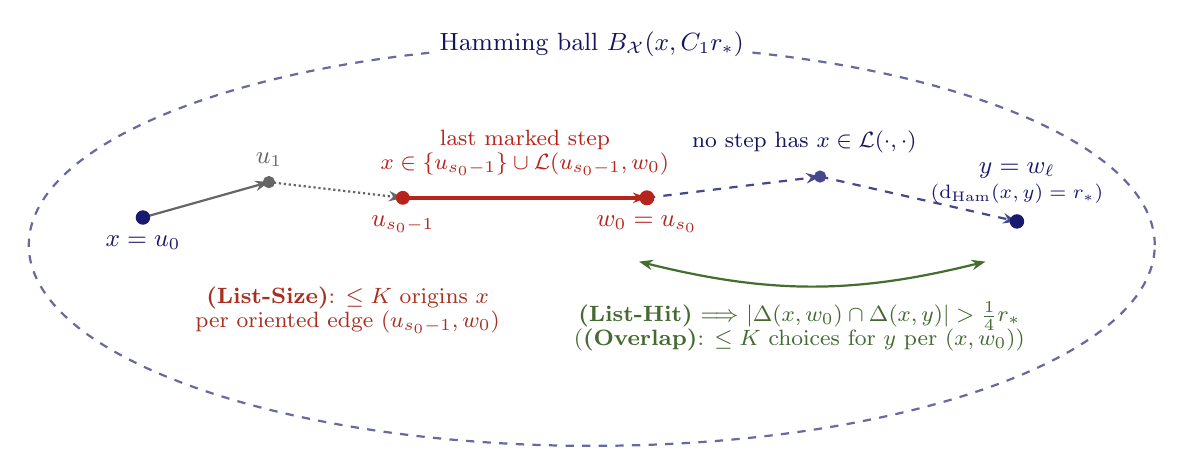
\begin{tikzpicture}[every node/.style={font=\small}, >={Stealth[length=5pt]}]
  % Outer ball B_X(x, C_1 r_*)
  \draw[dashed, thick, MidnightBlue!65] (5.35, -0.15) ellipse (7.15cm and 2.55cm);
  \node[MidnightBlue!85!black, fill=white, inner sep=1.5pt] at (5.35, 2.4) {Hamming ball $B_{\mathcal{X}}(x, C_1 r_*)$};

  % Nodes along the local path from x to y
  \coordinate (x) at (-0.35, 0.2);
  \coordinate (u1) at (1.25, 0.65);
  \coordinate (usprev) at (2.95, 0.45);
  \coordinate (w0) at (6.05, 0.45);
  \coordinate (w1) at (8.25, 0.72);
  \coordinate (y) at (10.75, 0.15);

  % Prefix path
  \draw[->, thick, gray!80!black] (x) -- (u1);
  \draw[->, thick, gray!80!black, densely dotted] (u1) -- (usprev);

  % Last marked step (u_{s_0 - 1}, w_0)
  \draw[->, ultra thick, BrickRed] (usprev) -- node[above=4pt, align=center, font=\footnotesize, text=BrickRed] {last marked step\\[-1pt]$x \in \{u_{s_0-1}\} \cup \mathcal{L}(u_{s_0-1}, w_0)$} (w0);

  % Unmarked suffix w_0 -> ... -> y
  \draw[->, thick, MidnightBlue!80, dashed] (w0) -- (w1);
  \draw[->, thick, MidnightBlue!80, dashed] (w1) -- (y);
  \node[MidnightBlue!85!black, above=4pt, align=center, font=\footnotesize] at (8.05, 0.76) {no step has $x \in \mathcal{L}(\cdot, \cdot)$};

  % Alignment curve from w_0 to y
  \draw[<->, thick, OliveGreen!80!black] (5.95, -0.36) to[bend right=14] node[below=2pt, pos=0.46, align=center, font=\footnotesize, text=OliveGreen!75!black] {\textbf{(List-Hit)} $\Longrightarrow$ $|\Delta(x, w_0) \cap \Delta(x, y)| > \tfrac{1}{4} r_*$\\[-1pt](\textbf{(Overlap)}: $\le K$ choices for $y$ per $(x, w_0)$)} (10.35, -0.36);

  % Callout for (List-Size)
  \node[BrickRed!90!black, align=center, font=\footnotesize] at (2.25, -0.98) {\textbf{(List-Size)}: $\le K$ origins $x$\\[-1pt]per oriented edge $(u_{s_0-1}, w_0)$};

  % Vertex markers
  \filldraw[MidnightBlue] (x) circle (2.4pt) node[below=3pt] {$x = u_0$};
  \filldraw[gray!80!black] (u1) circle (2.0pt) node[above=2pt] {$u_1$};
  \filldraw[BrickRed] (usprev) circle (2.3pt) node[below=3pt] {$u_{s_0-1}$};
  \filldraw[BrickRed] (w0) circle (2.5pt) node[below=3pt] {$w_0 = u_{s_0}$};
  \filldraw[MidnightBlue!80] (w1) circle (2.0pt);
  \filldraw[MidnightBlue] (y) circle (2.4pt) node[above=3pt, align=center] {$y = w_\ell$\\[-2pt]{\scriptsize ($\dHam(x, y) = r_*$)}};
\end{tikzpicture}
\caption{How a $K$-bounded list system bounds close pairs in Theorem~\ref{thm:mod2-combinatorial}(a). Along a local path from $x$ to $y$, let $(u_{s_0-1}, w_0)$ be the last step whose list (plus $\{u_{s_0-1}\}$) contains $x$. By~\textbf{(List-Size)}, the $2|\widehat{E}|$ oriented edges generate at most $2 K |\widehat{E}|$ hit pairs $(x, w_0)$. Because the remaining suffix from $w_0$ to $y$ never hits $x$'s list, the contrapositive of~\textbf{(List-Hit)} forces $w_0$ to be aligned with $y$ (unless $w_0 = y$), and~\textbf{(Overlap)} leaves at most $K$ possibilities for $y$, giving $|E_{r_*}(\mathcal{X})| \le 2 K^2 |\widehat{E}|$.}
\label{fig:list-charging}
\end{figure}

Part~(a) of the next theorem is the charging argument. Part~(b) is a statement about sequences of finite sets, which is the main tool for verifying Condition~\textbf{(List-Hit)} in Section~\ref{sec:csp-cloud}; there, $F_t = \Delta(x, w_t)$ is the set of coordinates in which the $t$-th vertex of a walk differs from $x$. Part~(b) considers sets $F_0, \dots, F_\ell$ of size at most $C_1 r_*$ whose first and last members share at most $\frac{1}{4} r_*$ elements. It finds a step $s$ at which $F_{s-1} \cap F_s$ partitions into $k \le k_{\max} = 8 C_1$ disjoint pieces $A_1, \dots, A_k$ and a remainder $I_k$ of size at most $\frac{1}{2} r_*$, together with sequence members $F_{t_1}, \dots, F_{t_k}$, such that each $F_{t_r}$ avoids $A_r$, covers the remaining pieces $I_r = A_{r+1} \sqcup \dots \sqcup A_k \sqcup I_k$, and contains at least $|A_r| - \frac{1}{4} r_*$ elements of $(F_{s-1} \cup F_s) \setminus (A_r \sqcup I_r)$. Crucially, $k_{\max}$ does not depend on the length $\ell$ of the sequence.

\begin{theorem}[Charging Argument and Set-Sequence Lemma; proved in Section~\ref{sec:combinatorics}]
\label{thm:mod2-combinatorial}
Let $C_1 \ge 2$ and $r_* \ge 1$ be integers, and set $k_{\max} := 8 C_1$.
\begin{enumerate}[label=(\alph*)]
  \item \emph{(Charging argument.)} Let $N, q \ge 2$ and $K \ge 1$ be integers, and let $\mathcal{X} \subseteq [q]^N$ be a code that admits a $K$-bounded list system with parameters $C_1$ and $r_*$. Then every $(C_1, r_*)$-local connector $\widehat{G} = (\mathcal{X}, \widehat{E})$ for $\mathcal{X}$ satisfies $|E_{r_*}(\mathcal{X})| \le 2 K^2\,|\widehat{E}|$.
  \item \emph{(Set-sequence lemma.)} Let $N \ge 1$ and $\ell \ge 1$ be integers, and let $F_0, F_1, \dots, F_\ell \subseteq [N]$ satisfy $|F_t| \le C_1 r_*$ ($0 \le t \le \ell$) and $|F_0 \cap F_\ell| \le \frac{1}{4} r_*$. Writing $W_s := F_{s-1} \cup F_s$, there exist $s \in \{1, \dots, \ell\}$, an integer $0 \le k \le k_{\max}$, indices $t_1, \dots, t_k \in \{0, \dots, \ell\}$, and pairwise disjoint subsets $A_1, \dots, A_k, I_k \subseteq F_{s-1} \cap F_s$ with $F_{s-1} \cap F_s = A_1 \sqcup \dots \sqcup A_k \sqcup I_k$ and $|I_k| \le \frac{1}{2} r_*$ such that, setting $I_{r-1} := A_r \sqcup \dots \sqcup A_k \sqcup I_k$ ($1 \le r \le k + 1$), every $1 \le r \le k$ satisfies
  \[
  A_r \cap F_{t_r} \;=\; \emptyset, \qquad I_r \;\subseteq\; F_{t_r}, \qquad \text{and} \qquad \bigl|(W_s \cap F_{t_r}) \setminus I_{r-1}\bigr| \;\ge\; |A_r| - \frac{1}{4}\,r_*.
  \]
\end{enumerate}
\end{theorem}

\subsection{Step 3: Codes with Many Close Pairs and Short Lists}
\label{subsec:mod3}

The third step provides the codes. Informally, for every sufficiently large $r_*$ there is a code of length $N = O_{C_1}(r_*)$ with $n = 2^{\Theta_{C_1}(r_*)}$ codewords, minimum distance at least $\frac{1}{2} r_*$, $\Omega(n^{1 + c})$ close pairs, and a $K$-bounded list system with $K = O(C_1^2)$. The theorem gives the constants explicitly; they are needed only in Section~\ref{subsec:master-proof}.

\begin{theorem}[Existence of Hard Codes; proved in Section~\ref{sec:csp-cloud}]
\label{thm:mod3-cloud}
For every integer $C_1 \ge 3$, there exist integer constants $L, q, K \ge 2$ and $R_0 > 160 C_1$ (with $L = O(C_1^3 \log C_1)$ and $K = 20 C_1^2$) and real constants $\mu_0 > 0$ and $c(C_1) := 2^{-(2 L + 5)} > 0$ such that for every integer $r_* \ge R_0$, setting $N := 2^L r_*$, there exists a code $\mathcal{X} \subseteq [q]^N$ of size $n := |\mathcal{X}| \ge 2$ with the following properties:
\begin{enumerate}[label=(\arabic*),nosep]
  \item $\frac{2}{5} \mu_0 r_* \le \log_2 n \le \frac{3}{2} \mu_0 r_*$ and $|E_{r_*}(\mathcal{X})| \ge \frac{1}{192}\,n^{1 + c(C_1)}$;
  \item $\dHam(x, y) \ge \frac{1}{2} r_*$ for all distinct $x, y \in \mathcal{X}$; and
  \item $\mathcal{X}$ admits a $K$-bounded list system with parameters $C_1$ and $r_*$.
\end{enumerate}
\end{theorem}

\subsection{Proofs of Theorems~\ref{thm:geometric} and~\ref{thm:main} and of Corollary~\ref{cor:lp-dvoretzky}}
\label{subsec:master-proof}

\begin{proof}[Proof of Theorem~\ref{thm:main} (and Theorem~\ref{thm:geometric}) from Theorems~\ref{thm:mod1-projection}--\ref{thm:mod3-cloud}]
Fix $p \in [1, \infty)$ and $C \ge 1$, and set $C_1 := \max(3, \lceil C^p \rceil)$. Let $L, q, K, R_0, \mu_0, c(C_1)$ be the constants of Theorem~\ref{thm:mod3-cloud} at $C_1$. For each integer $j \ge 1$, set $r_j := 4^j R_0 \ge R_0$ and $N_j := 2^L r_j$, let $\mathcal{X}_j \subseteq [q]^{N_j}$ be the code given by Theorem~\ref{thm:mod3-cloud} at $r_* = r_j$, put $n_j := |\mathcal{X}_j| \ge 2$, and define $P_{n_j} := \iota(\mathcal{X}_j) \subset \{0, 1\}^{d(n_j)}$ where $d(n_j) := N_j q = 2^L q r_j \ge 1$.
\begin{enumerate}[label=(\arabic*)]
  \item \emph{Dimension and aspect ratio:} By Theorem~\ref{thm:mod3-cloud}(1), $\log_2 n_{j+1} \ge \frac{2}{5} \mu_0 (4 r_j) = \frac{8}{5}\mu_0 r_j > \frac{3}{2} \mu_0 r_j \ge \log_2 n_j$, so $\{n_j\}_{j \ge 1}$ is strictly increasing with $n_1 \ge 2$, and $\frac{2}{5} \mu_0 r_j \le \log_2 n_j \le \frac{3}{2} \mu_0 r_j$ gives
  \[
  \beta_1(C_1)\log_2 n_j \;:=\; \frac{2 \cdot 2^L q}{3 \mu_0} \log_2 n_j \;\le\; d(n_j) \;=\; 2^L q r_j \;\le\; \frac{5 \cdot 2^L q}{2 \mu_0} \log_2 n_j \;=:\; \beta_2(C_1)\log_2 n_j,
  \]
  so $d(n_j) = \Theta_{C, p}(\log n_j)$ with $0 < \beta_1(C_1) < \beta_2(C_1)$. By Theorem~\ref{thm:mod3-cloud}(2) and Theorem~\ref{thm:mod1-projection}(b), $P_{n_j} \subset \{0, 1\}^{d(n_j)}$ has $n_j$ distinct points and aspect ratio $\Delta_p(P_{n_j}) \le 2^{L+1} =: A(C_1)$.
  \item \emph{Spanner size lower bound:} Let $H = (P_{n_j} \sqcup S, E, w)$ be any Steiner $C$-spanner of $(P_{n_j}, \|\cdot\|_p)$. Since $C_1 \ge \lceil C^p \rceil$ and $\mathcal{X}_j$ has minimum distance at least $\frac{1}{2} r_j$ by Theorem~\ref{thm:mod3-cloud}(2), Theorem~\ref{thm:mod1-projection}(b) provides a $(C_1, r_j)$-local connector $\widehat{G} = (\mathcal{X}_j, \widehat{E})$ for $\mathcal{X}_j$ with $|\widehat{E}| \le |E|$. Since $N_j, q \ge 2$, $r_j \ge 1$, $C_1 \ge 2$, and $\mathcal{X}_j$ admits a $K$-bounded list system with parameters $C_1$ and $r_j$ by Theorem~\ref{thm:mod3-cloud}(3), Theorem~\ref{thm:mod2-combinatorial}(a) applies to $\widehat{G}$, and together with Theorem~\ref{thm:mod3-cloud}(1) it yields
  \[
  |E| \;\ge\; |\widehat{E}| \;\ge\; \frac{|E_{r_j}(\mathcal{X}_j)|}{2 K^2} \;\ge\; \frac{1}{384 K^2}\,n_j^{1 + c(C_1)}.
  \]
  Set $c_0(C_1) := (384 K^2)^{-1} > 0$. Since $L = O(C_1^3 \log C_1)$, $C_1 = \max(3, \lceil C^p \rceil) \le 3 C^p$, and $\log_2 C_1 \le \log_2(3 C^p) < 3\log_2(C^p + 1)$ for all $C, p \ge 1$, we have $c(C_1) = 2^{-(2L + 5)} = 2^{-O(C_1^3 \log C_1)} = 2^{-O(C^{3p}\log(C^p + 1))}$ with absolute implicit constants (giving $2^{-O(C^3 \log(C + 1))}$ at $p = 1$, and $2^{-O(C^6 \log(C + 1))}$ at $p = 2$ since $\log_2(C^2 + 1) \le 2\log_2(C + 1)$). This proves Theorem~\ref{thm:main}. Theorem~\ref{thm:geometric} follows with $c(C, p) := c(C_1)$ and $c_0(C, p) := c_0(C_1)$, because every geometric $C$-spanner is a Steiner $C$-spanner with $S = \emptyset$. \qedhere
\end{enumerate}
\end{proof}

\begin{proof}[Proof of Corollary~\ref{cor:lp-dvoretzky}]
Apply Theorem~\ref{thm:main} at $p_0 = 2$ and stretch $2 C$ to obtain $n$-point sets $Q_n \subset \{0, 1\}^{d_2(n)}$ with $d_2(n) = \Theta_C(\log n)$, $\Delta_2(Q_n) = O_C(1)$, and $(2C)$-spanner lower bound $c_0(C)\,n^{1 + c(C)}$ where $c(C) = 2^{-O((2C)^6 \log((2C)^2 + 1))} = 2^{-O(C^6 \log(C + 1))}$. By~\cite[Example~3.1]{figiel1977dimension}, there is a linear map $T : \R^{d_2(n)} \to \R^{d(n)}$ with $d(n) = \Theta_p\bigl(d_2(n)^{p/2}\bigr) = \Theta_{C, p}\bigl((\log n)^{p/2}\bigr)$ satisfying $\|v\|_2 \le \|T v\|_p \le 2\,\|v\|_2$ for all $v \in \R^{d_2(n)}$. Setting $P_n := T(Q_n)$ gives $|P_n| = n$ and $\Delta_p(P_n) \le 2\,\Delta_2(Q_n) = O_C(1)$, and pulling any Steiner $C$-spanner of $(P_n, \|\cdot\|_p)$ back along $T$ (keeping the same edge set and weights) yields a Steiner $(2C)$-spanner of $(Q_n, \|\cdot\|_2)$.
\end{proof}


% ============================================================================
\section{Warm-Ups: What Steiner Vertices and Three Hops Can Do}
\label{sec:warmups}
% ============================================================================

Before proving Theorems~\ref{thm:mod1-projection}--\ref{thm:mod3-cloud}, we record three elementary constructions. They illustrate the power of Steiner vertices and of paths with more than two edges, and they explain two features of the codes constructed in Section~\ref{sec:csp-cloud}: the distance $r_*$ of the close pairs is only a small fraction $r_*/N = 2^{-L}$ of the length of the code (Proposition~\ref{prop:simplex}(b)), and the codes are far from being dense subsets of the hypercube (Proposition~\ref{prop:three-hop}). Throughout this section, recall from Definition~\ref{def:spanner} that a spanner $H = (P \sqcup S, E, w)$ of $(P, \dP)$ is a \emph{$k$-hop} $C$-spanner if every pair of distinct terminals $x, y \in P$ is connected in $H$ by a simple path of at most $k$ edges and weight at most $C \cdot \dP(x, y)$. None of the results in this section are needed in Sections~\ref{sec:projection}--\ref{sec:csp-cloud}.

\subsection{Buckets and Equidistant Points}
\label{subsec:bucketing-simplex}

A family of clusters or hash buckets gives a graph with one Steiner vertex per bucket, joined to the points of the bucket; the number of edges is the total size $\sum_{i \in I} |B_i|$ of the buckets. If every pair of points shares a bucket of suitable diameter, this graph is a $2$-hop Steiner spanner. For a single bucket it is the star of~\cite{andoni2023subquadratic}.

\begin{proposition}[Buckets Give $2$-Hop Steiner Spanners]
\label{prop:bucketing}
Let $(P, \dP)$ be a finite metric space with $|P| \ge 2$, let $C \ge 1$, and let $(B_i)_{i \in I}$ be a finite indexed family of subsets $B_i \subseteq P$ with $|B_i| \ge 2$ and diameter $D_i := \max_{u, v \in B_i} \dP(u, v) > 0$. Define the bipartite weighted graph $H = (P \sqcup S, E, w)$, where $S := \{s_i : i \in I\}$ consists of $|I|$ distinct auxiliary vertices disjoint from $P$, $E := \{\{x, s_i\} : i \in I,\, x \in B_i\}$, and $w(\{x, s_i\}) := \frac{1}{2} D_i$.
\begin{enumerate}[label=(\alph*),nosep]
  \item $|E| = \sum_{i \in I} |B_i|$ and $\dH(x, y) \ge \dP(x, y)$ for all $x, y \in P$.
  \item If for every pair of distinct points $x, y \in P$ there exists $i \in I$ with $\{x, y\} \subseteq B_i$ and $D_i \le C \cdot \dP(x, y)$, then $H$ is a $2$-hop Steiner $C$-spanner of $(P, \dP)$.
\end{enumerate}
\end{proposition}

\begin{proof}
Each $s_i \in S$ has degree $|B_i|$ into $P$ and $P, S$ are independent sets in $H$, so $H$ is finite and simple with $|E| = \sum_{i \in I} |B_i|$. For~(a), if $x = y \in P$ then $\dH(x, x) = 0 = \dP(x, x)$. If $x \ne y \in P$, any walk $(v_0 = x, v_1, \dots, v_k = y)$ in $H$ alternates between $P$ and $S$, so $k = 2m$ ($m \ge 1$) with $v_{2t} \in P$ ($0 \le t \le m$) and $v_{2t-1} = s_{i_t} \in S$ ($1 \le t \le m$) satisfying $\{v_{2t-2}, v_{2t}\} \subseteq B_{i_t}$. For each $1 \le t \le m$,
\[
w(\{v_{2t-2}, s_{i_t}\}) + w(\{s_{i_t}, v_{2t}\}) \;=\; \frac{1}{2} D_{i_t} + \frac{1}{2} D_{i_t} \;=\; D_{i_t} \;\ge\; \dP(v_{2t-2}, v_{2t}).
\]
Summing over $1 \le t \le m$ and applying the triangle inequality in $(P, \dP)$ yields $\sum_{j=1}^k w(\{v_{j-1}, v_j\}) \ge \dP(x, y)$; taking the infimum over all $(x, y)$-walks gives $\dH(x, y) \ge \dP(x, y)$. For~(b), given $x \ne y \in P$, choosing $i \in I$ with $\{x, y\} \subseteq B_i$ and $D_i \le C \cdot \dP(x, y)$ gives the simple $2$-hop path $(x, s_i, y)$ of weight $\frac{1}{2} D_i + \frac{1}{2} D_i = D_i \le C \cdot \dP(x, y)$.
\end{proof}

With a single bucket that contains all points, Proposition~\ref{prop:bucketing} has two consequences, in every $\ell_p$ norm. First, $n$ equidistant points have a Steiner spanner with $n$ edges and stretch $1$, although every geometric spanner of stretch below $2$ needs all $\binom{n}{2}$ edges (and metric Steiner spanners in Euclidean space need $n^{2 - o(1)}$ edges for stretch below $\sqrt{2}$~\cite{andoni2023subquadratic}). Second, a code of length $N$ and minimum distance $r_0$ has a Steiner spanner with stretch $(N / r_0)^{1/p}$ and one edge per codeword. Hence the codes in our lower bound must have $N > C^p r_0$.

\begin{proposition}[Equidistant Points, and the Necessity of $N > C^p r_0$]
\label{prop:simplex}
Let $p \in [1, \infty)$.
\begin{enumerate}[label=(\alph*),nosep]
  \item Let $n \ge 3$ and $P := \{e_1, \dots, e_n\} \subset \{0, 1\}^n$ be the standard basis ($\|e_i - e_j\|_p = 2^{1/p}$ for $i \ne j$). Every geometric $C$-spanner of $(P, \|\cdot\|_p)$ with $1 \le C < 2$ has $\binom{n}{2}$ edges, whereas $(P, \|\cdot\|_p)$ admits a $2$-hop Steiner $1$-spanner with $n$ edges.
  \item For any integers $N, q \ge 2$, $r_0 \ge 1$, and any $\mathcal{X} \subseteq [q]^N$ ($|\mathcal{X}| \ge 2$) with $\min_{x \ne y \in \mathcal{X}} \dHam(x, y) \ge r_0$, the one-hot point set $\iota(\mathcal{X}) \subset \{0, 1\}^{N q}$ admits a $2$-hop Steiner $(N / r_0)^{1/p}$-spanner with $|\mathcal{X}|$ edges.
\end{enumerate}
\end{proposition}

\begin{proof}
For~(a), if $1 \le C < 2$, any walk in a geometric spanner of $(P, \|\cdot\|_p)$ between $e_i$ and $e_j$ ($i \ne j$) avoiding the edge $\{e_i, e_j\}$ traverses at least two edges between distinct vertices of $P$ and thus has weight at least $2 \cdot 2^{1/p} > C \|e_i - e_j\|_p$, forcing all $\binom{n}{2}$ edges to be present~\cite{andoni2023subquadratic}, whereas Proposition~\ref{prop:bucketing} with $B_1 = P$ gives $n$ edges at stretch $1$. For~(b), Proposition~\ref{prop:bucketing} applied to $(\iota(\mathcal{X}), \|\cdot\|_p)$ with $B_1 = \iota(\mathcal{X})$ has diameter $D_1 = \max_{u, v \in \mathcal{X}} (2\,\dHam(u, v))^{1/p} \le (2 N)^{1/p} = (N / r_0)^{1/p} (2 r_0)^{1/p} \le (N / r_0)^{1/p} \|\iota(x) - \iota(y)\|_p$ for all $x \ne y \in \mathcal{X}$, giving stretch $(N / r_0)^{1/p}$ with $|\iota(\mathcal{X})| = |\mathcal{X}|$ edges.
\end{proof}

\subsection{Three Hops in Dense Subsets of the Hypercube}
\label{subsec:three-hop}

Why not prove Theorem~\ref{thm:main} on $\{0, 1\}^d$ or on a dense subset of it? On $\{0, 1\}^d$ ($n = 2^d$), $2$-hop spanners achieving constant stretch $C$ require $n^{1 + \Omega(1/C^2)}$ edges in $\ell_2$~\cite{harpeled2013euclidean}, and $2$-hop non-metric Steiner $C$-spanners require $n^{1 + \Omega(1/C^p)}$ edges in every $\ell_p$ norm (in particular, $n^{1 + \Omega(1/C)}$ in $\ell_1$)~\cite[Theorem~1.2 and Remark~3.2]{krauthgamer2026towards}. Once a third hop is permitted, however, Krauthgamer and Petruschka~\cite[Theorem~A.1]{krauthgamer2026towards} proved that binary Hamming codes span the full cube $(\{0, 1\}^d, \|\cdot\|_1)$ at stretch $128$ in $O(2^d \log d)$ edges. Their bound on the number of edges is in terms of $2^d$ and not of $|P|$, so it says nothing about a subset $P \subsetneq \{0, 1\}^d$ with $|P| = 2^{(1 - \varepsilon) d}$. We show that the same construction, with a smaller distance threshold between codewords, works for every sufficiently dense subset $P \subseteq \{0, 1\}^d$, in every $\ell_p$ norm, with a stretch that is an absolute constant:

\begin{lemma}[Three-Hop Paths at One Distance Scale]
\label{lem:hamming-layer}
Let $r \ge 4$ and $d \ge 1$ be integers, let $p \in [1, \infty)$, and set $b_r := 2^r - 1$ and $\rho_r := \frac{1}{64 b_r}$. For every subset $P \subseteq \{0, 1\}^d$ with $|P| \ge 2$ and $|P| \ge 2^{(1 - \frac{r}{2 b_r}) d}$, there exists a weighted simple graph $H_r = (P \sqcup S_r, E_r, w)$ with $S_r \subseteq \{0, 1\}^d \setminus P$ and $w(\{u, v\}) = \|u - v\|_p$ such that $|E_r| \le 2|P|$, $\mathrm{d}_{H_r}(x, y) \ge \|x - y\|_p$ for all $x, y \in P$, and every pair $x, y \in P$ with $\frac{1}{3}\rho_r d \le \dHam(x, y) \le \frac{9}{4}\rho_r d$ is connected in $H_r$ by a simple path of at most $3$ edges and weight at most $387\,\|x - y\|_p$.
\end{lemma}

\begin{proof}
Because $H_r$ will take $P \sqcup S_r \subseteq \{0, 1\}^d$ and $w(\{u, v\}) = \|u - v\|_p$, non-contraction $\mathrm{d}_{H_r}(x, y) \ge \|x - y\|_p$ holds automatically for all $x, y \in P$ by the $\ell_p$ triangle inequality. If $\frac{9}{4}\rho_r d < 1$, no pair $x, y \in P$ has integer Hamming distance in $[\frac{1}{3}\rho_r d, \frac{9}{4}\rho_r d]$, so $S_r = \emptyset$ and $E_r = \emptyset$ satisfy the claim trivially. Assume henceforth that $\frac{9}{4}\rho_r d \ge 1$, so $d \ge \frac{4}{9 \rho_r} = \frac{256}{9} b_r > 28 b_r$.

Let $A_r \in \mathbb{F}_2^{r \times b_r}$ be the matrix whose columns are the $b_r = 2^r - 1$ nonzero vectors of $\mathbb{F}_2^r$, and let $\mathcal{H}_{b_r} := \{z \in \{0, 1\}^{b_r} : A_r z = 0 \text{ in } \mathbb{F}_2^r\}$ be the binary Hamming code. Since $A_r$ contains the $r$ standard basis vectors, $\operatorname{rank}_{\mathbb{F}_2}(A_r) = r$ and $|\mathcal{H}_{b_r}| = 2^{b_r - r}$. For each $u \in \{0, 1\}^{b_r}$, if $A_r u = 0$ set $\psi_{\mathrm{blk}}(u) := u \in \mathcal{H}_{b_r}$; otherwise $A_r u \in \mathbb{F}_2^r \setminus \{0\}$ equals a unique column $j$ of $A_r$, and flipping $u_j$ yields $\psi_{\mathrm{blk}}(u) \in \mathcal{H}_{b_r}$ with $\dHam(u, \psi_{\mathrm{blk}}(u)) = 1$ (note $\psi_{\mathrm{blk}}(z) = z$ for all $z \in \mathcal{H}_{b_r}$).

Write $d = M b_r + q_0$ with integers $M = \lfloor d / b_r \rfloor \ge 28$ and $0 \le q_0 < b_r$. Partition $[d]$ into $M$ blocks of length $b_r$ plus a remainder block of length $q_0$, set $\mathcal{C}_r := (\mathcal{H}_{b_r})^M \times \{0, 1\}^{q_0} \subseteq \{0, 1\}^d$, and define $\psi_r : \{0, 1\}^d \to \mathcal{C}_r$ by applying $\psi_{\mathrm{blk}}$ to each of the $M$ blocks of length $b_r$ and leaving the last $q_0$ coordinates unchanged (so $\psi_r(c) = c$ for all $c \in \mathcal{C}_r$). Then:
\begin{enumerate}[label=(\arabic*),nosep]
  \item For every $x \in \{0, 1\}^d$, $\dHam(x, \psi_r(x)) \le M \le \frac{d}{b_r} = 64 \rho_r d$.
  \item For every $x, y \in \{0, 1\}^d$, on each block $B$ where $x|_B = y|_B$ we have $\psi_r(x)|_B = \psi_r(y)|_B$. On each of the $M$ length-$b_r$ blocks where $\dHam(x|_B, y|_B) \ge 1$, the triangle inequality gives $\dHam(\psi_{\mathrm{blk}}(x|_B), \psi_{\mathrm{blk}}(y|_B)) \le 1 + \dHam(x|_B, y|_B) + 1 \le 3\,\dHam(x|_B, y|_B)$, while on the remainder block $B_{\mathrm{rem}}$ we have $\psi_r(x)|_{B_{\mathrm{rem}}} = x|_{B_{\mathrm{rem}}}$ and $\psi_r(y)|_{B_{\mathrm{rem}}} = y|_{B_{\mathrm{rem}}}$. Summing over blocks yields $\dHam(\psi_r(x), \psi_r(y)) \le 3\,\dHam(x, y)$.
\end{enumerate}
Set $S_r := \mathcal{C}_r \setminus P$, let $k := \lfloor \frac{27}{4}\rho_r d \rfloor \le 7 \rho_r d$, and define
\[
E_r \;:=\; \bigl\{\{x, \psi_r(x)\} : x \in P,\, \psi_r(x) \ne x\bigr\} \;\cup\; \Bigl\{\{c, c'\} \in \binom{\mathcal{C}_r}{2} : 1 \le \dHam(c, c') \le k\Bigr\}.
\]
For any $x, y \in P$ with $\frac{1}{3}\rho_r d \le \dHam(x, y) \le \frac{9}{4}\rho_r d$, we have $x \ne y$; property~(1) gives both $\dHam(x, \psi_r(x)) \le 64 \rho_r d \le 192\,\dHam(x, y)$ and $\dHam(y, \psi_r(y)) \le 192\,\dHam(x, y)$, while property~(2) gives $\dHam(\psi_r(x), \psi_r(y)) \le 3\,\dHam(x, y) \le k$, so either $\psi_r(x) = \psi_r(y)$ or the pair $\{\psi_r(x), \psi_r(y)\}$ lies in $E_r$. Since $\psi_r$ is idempotent, $x = \psi_r(y)$ implies $\psi_r(x) = x$, and $\psi_r(x) = y$ implies $\psi_r(y) = y$; hence deleting consecutive duplicates from $(x, \psi_r(x), \psi_r(y), y)$ eliminates all repeated vertices and yields a simple path in $H_r$ of at most $3$ edges and weight at most
\[
\|x - \psi_r(x)\|_p + \|\psi_r(x) - \psi_r(y)\|_p + \|\psi_r(y) - y\|_p \le \bigl(192^{1/p} + 3^{1/p} + 192^{1/p}\bigr)\dHam(x, y)^{1/p} \le 387\|x - y\|_p.
\]
Finally, to bound $|E_r|$, the first set in $E_r$ has size at most $|P|$. For the second set, if $k = 0$ it is empty; if $k \ge 1$, then since $\sum_{j=1}^k \binom{d}{j} (k/d)^k \le \sum_{j=0}^d \binom{d}{j}(k/d)^j = (1 + k/d)^d \le e^k$ and $t \mapsto (e d / t)^t$ is increasing on $(0, d]$, we have $\sum_{j=1}^k \binom{d}{j} \le (e d / k)^k \le (64 e b_r / 7)^{7 \rho_r d}$. Using $64 e / 7 < 32 = 2^5$, $b_r < 2^r$, and $r \ge 4$ gives $\log_2(64 e b_r / 7) < r + 5 \le \frac{9}{4} r$, so $7 \rho_r \log_2(64 e b_r / 7) < \frac{63}{256} \frac{r}{b_r} < \frac{r}{4 b_r}$. Since $|\mathcal{C}_r| = 2^{d - M r}$ with $M > d/b_r - 1$ and $d > 28 b_r$, the number of codeword edges is at most
\[
\frac{1}{2}|\mathcal{C}_r|\sum_{j=1}^k \binom{d}{j} \;\le\; 2^{(1 - \frac{r}{b_r}) d + r - 1 + \frac{r}{4 b_r} d} \;<\; 2^{(1 - \frac{r}{2 b_r}) d} \;\le\; |P|,
\]
where the strict inequality uses $\frac{r}{4 b_r} d > 7 r > r - 1$. Thus $|E_r| \le 2|P|$.
\end{proof}

\begin{proposition}[Three-Hop Paths in Dense Subsets of the Hypercube]
\label{prop:three-hop}
Let $p \in [1, \infty)$ and $\rho \in (0, 1)$. There exists $\varepsilon(\rho) > 0$ such that for every integer $d \ge 1$ and every subset $P \subseteq \{0, 1\}^d$ with $|P| \ge 2$ and $|P| \ge 2^{(1 - \varepsilon(\rho)) d}$:
\begin{enumerate}[label=(\alph*),nosep]
  \item There is a weighted simple graph $H = (P \sqcup S, E, w)$ with $S \subseteq \{0, 1\}^d \setminus P$, $w(\{u, v\}) = \|u - v\|_p$, $|E| \le 2|P|$, and $\dH(x, y) \ge \|x - y\|_p$ for all $x, y \in P$ in which every pair $x, y \in P$ with $\frac{1}{3}\rho d \le \dHam(x, y) \le \rho d$ is connected by a simple path of at most $3$ edges and weight at most $5760\,\|x - y\|_p$.
  \item If in addition $\min_{x \ne y \in P} \dHam(x, y) \ge \frac{1}{3}\rho d$, then $(P, \|\cdot\|_p)$ admits a $3$-hop metric Steiner $5760$-spanner (in ambient space $(\{0, 1\}^d, \|\cdot\|_p)$) with at most $2|P|\log_2(2/\rho)$ edges. In particular, for $d \ge 2$, taking $P = \{0, 1\}^d$ and $\rho = \min(\frac{1}{2}, \frac{3}{d})$ recovers a $3$-hop geometric $O(1)$-spanner of $(\{0, 1\}^d, \|\cdot\|_p)$ ($S = \emptyset$) with $O(2^d \log d)$ edges~\cite[Theorem~A.1]{krauthgamer2026towards}.
\end{enumerate}
\end{proposition}

\begin{proof}
Write $E_{\mathrm{top}} := \{\{x, 0^d\} : x \in P \setminus \{0^d\}\}$ weighted by $\|\cdot\|_p$; note $|E_{\mathrm{top}}| \le |P|$, and for every $x, y \in P$ with $\dHam(x, y) > \frac{1}{2880} d$ (hence $x \ne y$), routing via $0^d$ yields a simple path ($(x, y)$ if $0^d \in \{x, y\}$, and $(x, 0^d, y)$ otherwise) of at most $2$ edges and weight at most $\|x - 0^d\|_p + \|0^d - y\|_p \le 2 d^{1/p} \le 2 \cdot 2880^{1/p}\|x - y\|_p \le 5760\,\|x - y\|_p$.

If $\rho > \frac{1}{960}$, set $\varepsilon(\rho) := \frac{1}{2}$ and take $E := E_{\mathrm{top}}$ ($S := \{0^d\} \setminus P$). Every pair with $\dHam(x, y) \ge \frac{1}{3}\rho d > \frac{1}{2880} d$ is connected by a simple path of at most $2$ edges and weight at most $5760\,\|x - y\|_p$, and $|E| \le |P| \le 2|P|\log_2(2/\rho)$ since $\log_2(2/\rho) > 1$ for all $\rho \in (0, 1)$.

If $0 < \rho \le \frac{1}{960}$, since $\rho_r = \frac{1}{64(2^r - 1)}$ is strictly decreasing in $r$ with $\rho_4 = \frac{1}{960}$ and $\rho_3 = \frac{1}{448}$, there is a unique integer $r_0 \ge 4$ with $\rho_{r_0} \le \rho < \rho_{r_0 - 1}$. Set $\varepsilon(\rho) := \frac{r_0}{2 b_{r_0}} > 0$. Because $r \mapsto \frac{r}{2(2^r - 1)}$ is strictly decreasing for $r \ge 4$, $|P| \ge 2^{(1 - \varepsilon(\rho)) d}$ implies $|P| \ge 2^{(1 - \frac{r}{2 b_r}) d}$ for all $4 \le r \le r_0$. Also, for every $r \ge 4$, $\frac{\rho_{r-1}}{\rho_r} = \frac{2^r - 1}{2^{r-1} - 1} \le \frac{15}{7} < \frac{9}{4}$.
\begin{itemize}[leftmargin=2em,nosep]
  \item For~(a), $[\frac{1}{3}\rho d, \rho d] \subseteq [\frac{1}{3}\rho_{r_0} d, \frac{9}{4}\rho_{r_0} d]$, so Lemma~\ref{lem:hamming-layer} at $r = r_0$ gives $|E_{r_0}| \le 2|P|$ and simple paths of at most $3$ edges and stretch $387 \le 5760$.
  \item For~(b), take $S := \bigl(\{0^d\} \cup \bigcup_{r \in I_{\mathrm{act}}} S_r\bigr) \setminus P$ and $E := E_{\mathrm{top}} \cup \bigcup_{r \in I_{\mathrm{act}}} E_r$ over $I_{\mathrm{act}} := \{r \in \{4, \dots, r_0\} : \frac{9}{4}\rho_r d \ge 1\}$, weighted by $\|\cdot\|_p$ on $\{0, 1\}^d$ (hence globally non-contractive). Any distinct $x, y \in P$ satisfies $\dHam(x, y) \ge \max(1, \frac{1}{3}\rho_{r_0} d)$. If $\dHam(x, y) > \frac{9}{4}\rho_4 d = \frac{3}{1280} d > \frac{1}{2880} d$, $E_{\mathrm{top}}$ connects $(x, y)$ by a simple path of at most $2$ edges with stretch $5760$. Otherwise $\dHam(x, y) \in [\frac{1}{3}\rho_{r_0} d, \frac{9}{4}\rho_4 d]$; since $\frac{9}{4}\rho_r > \rho_{r-1} > \frac{1}{3}\rho_{r-1}$ for $5 \le r \le r_0$, the intervals $[\frac{1}{3}\rho_r d, \frac{9}{4}\rho_r d]$ cover $[\frac{1}{3}\rho_{r_0} d, \frac{9}{4}\rho_4 d]$, so some $r \in \{4, \dots, r_0\}$ satisfies $\frac{1}{3}\rho_r d \le \dHam(x, y) \le \frac{9}{4}\rho_r d$ (hence $\frac{9}{4}\rho_r d \ge 1$ and $r \in I_{\mathrm{act}}$), connecting $(x, y)$ by a simple path of at most $3$ edges with stretch $387 \le 5760$. Since $\rho < \rho_{r_0 - 1} = \frac{1}{64(2^{r_0 - 1} - 1)} < 2^{-(r_0 + 4)}$, we have $r_0 < \log_2(2/\rho)$ and $|E| \le |P| + 2(r_0 - 3)|P| < 2 r_0 |P| < 2|P|\log_2(2/\rho)$. For $P = \{0, 1\}^d$ ($d \ge 2$), $S \subseteq \{0, 1\}^d \setminus P = \emptyset$ and $\log_2(2/\rho) = O(\log d)$. \qedhere
\end{itemize}
\end{proof}


% ============================================================================
\section{Proof of Step 1: The Nearest-Terminal Map and the One-Hot Embedding}
\label{sec:projection}
% ============================================================================

This section proves Theorem~\ref{thm:mod1-projection} using only Definition~\ref{def:spanner} and elementary properties of shortest paths in finite non-negatively weighted graphs.

\subsection{The Nearest-Terminal Map}
\label{subsec:nearest-terminal}

To eliminate Steiner vertices without increasing the number of edges, we map every vertex of $H$ to a nearest terminal. This map is Mehlhorn's graph Voronoi partition~\cite{mehlhorn1988faster}, which was introduced to speed up the Steiner-tree approximation algorithm of Kou, Markowsky, and Berman~\cite{kou1981fast}. In the weighted Steiner Point Removal problem, by contrast, removing Steiner vertices via graph minors requires distortion $8 - o(1)$ even on trees~\cite{chan2006steiner} and $\tilde{\Omega}(\sqrt{\log |P|})$ in general graphs~\cite{chen2024lower}, while distortion $O(\log |P|)$ is achievable~\cite{filtser2019steiner}; the nearest-terminal map itself can incur weighted stretch $\Omega(|P|)$ on a comb~\cite{filtser2019steiner}. Theorem~\ref{thm:mod1-projection}(a) uses Mehlhorn's per-edge argument~\cite{mehlhorn1988faster} for a weaker goal, for which no such loss occurs: instead of preserving weighted distances, it keeps only \emph{unweighted} connectivity at a single scale, inside the ball $B_P(x, C r)$ and through edges of $\dP$-length at most $C r$. Each projected vertex and each projected edge is bounded individually against the total length $\dH(x, y) \le C r$ of a shortest path (Figure~\ref{fig:projection}).

\begin{figure}[ht]
\centering
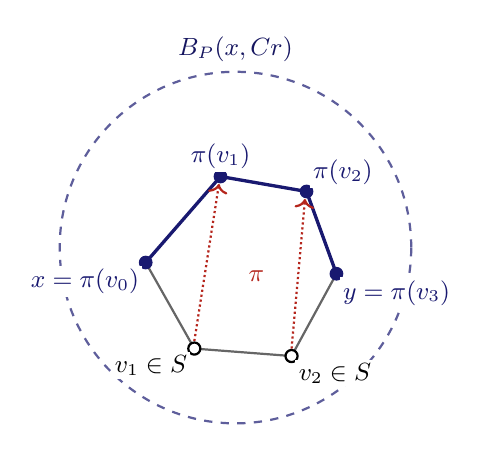
\begin{tikzpicture}[scale=0.95, every node/.style={font=\small}]
  % Ball B_P(x, C r)
  \draw[dashed, thick, MidnightBlue!70] (0,0) circle (2.35cm);
  \node[MidnightBlue!85!black] at (0, 2.65) {$B_P(x, C r)$};

  % Shortest path in H
  \draw[thick, gray!80!black] (-1.2, -0.2) -- (-0.55, -1.35) -- (0.75, -1.45) -- (1.35, -0.35);

  % Projected edges in \widehat{G}
  \draw[very thick, MidnightBlue] (-1.2, -0.2) -- (-0.2, 0.95) -- (0.95, 0.75) -- (1.35, -0.35);

  % Nearest-terminal projection arrows
  \draw[->, densely dotted, thick, BrickRed] (-0.55, -1.25) -- (-0.22, 0.85);
  \draw[->, densely dotted, thick, BrickRed] (0.75, -1.35) -- (0.93, 0.65);
  \node[BrickRed, fill=white, inner sep=1.2pt] at (0.28, -0.38) {$\pi$};

  % Terminals in P (drawn after edges so white label backgrounds stay legible)
  \filldraw[MidnightBlue] (-1.2, -0.2) circle (2.4pt) node[below left=1pt, fill=white, inner sep=1.2pt] {$x = \pi(v_0)$};
  \filldraw[MidnightBlue] (-0.2, 0.95) circle (2.4pt) node[above=1.5pt, fill=white, inner sep=1.2pt] {$\pi(v_1)$};
  \filldraw[MidnightBlue] (0.95, 0.75) circle (2.4pt) node[above right=1pt, fill=white, inner sep=1.2pt] {$\pi(v_2)$};
  \filldraw[MidnightBlue] (1.35, -0.35) circle (2.4pt) node[below right=1pt, fill=white, inner sep=1.2pt] {$y = \pi(v_3)$};

  % Steiner vertices outside / arbitrary
  \draw[fill=white, thick] (-0.55, -1.35) circle (2.3pt) node[below left=1pt, fill=white, inner sep=1.2pt] {$v_1 \in S$};
  \draw[fill=white, thick] (0.75, -1.45) circle (2.3pt) node[below right=1pt, fill=white, inner sep=1.2pt] {$v_2 \in S$};
\end{tikzpicture}
\caption{The nearest-terminal map $\pi : P \sqcup S \to P$ sends any shortest $(x, y)$-path $(v_0, v_1, v_2, v_3)$ in $H$ (solid gray) onto a walk $(\pi(v_0), \pi(v_1), \pi(v_2), \pi(v_3))$ inside $B_P(x, C r)$ in the unweighted terminal graph $\widehat{G}$ (thick blue), using $\dH(v_i, \pi(v_i)) \le \min\bigl(\dH(v_i, x), \dH(v_i, y)\bigr)$.}
\label{fig:projection}
\end{figure}

\begin{proof}[Proof of Theorem~\ref{thm:mod1-projection}(a)]
Because $P$ is finite and nonempty, for every $u \in P \sqcup S$ we may select a terminal $\pi(u) \in P$ minimizing $z \mapsto \dH(u, z)$ in $[0, \infty]$ over $z \in P$ (breaking ties arbitrarily; if $\dH(u, z) = \infty$ for all $z \in P$, $\pi(u)$ is any element of $P$). For every terminal $x \in P$, we have $\dH(x, x) = 0$, whereas for every $z \in P \setminus \{x\}$ spanner non-contraction and metric positivity give $\dH(x, z) \ge \dP(x, z) > 0$; thus $z = x$ is the unique minimizer and $\pi(x) = x$.

Define the subset of active edges $E' := \bigl\{\{u, v\} \in E : \pi(u) \ne \pi(v) \text{ and } \dP(\pi(u), \pi(v)) \le C r\bigr\}$ and set
\[
\widehat{E} \;:=\; \bigl\{\{\pi(u), \pi(v)\} : \{u, v\} \in E'\bigr\} \;\subseteq\; \binom{P}{2}, \qquad \widehat{G} \;:=\; (P, \widehat{E}).
\]
The map $\{u, v\} \mapsto \{\pi(u), \pi(v)\}$ sends $E'$ onto $\widehat{E}$, so $|\widehat{E}| \le |E'| \le |E|$, and by definition every $\{a, b\} \in \widehat{E}$ satisfies $a \ne b$ (hence $\dP(a, b) > 0$) and $\dP(a, b) \le C r$.

Now fix $x, y \in P$ with $0 < \dP(x, y) \le r$. Then $x \ne y$ and $\dH(x, y) \le C \dP(x, y) \le C r < \infty$. Because $H$ is finite and $w \ge 0$, $\dH$ is symmetric and satisfies the triangle inequality on $[0, \infty]$, and $\dH(x, y)$ is attained by a simple path $(v_0 = x, v_1, \dots, v_k = y)$ ($k \ge 1$) in $H$ with $\sum_{j=1}^k w(\{v_{j-1}, v_j\}) = \dH(x, y)$~\cite[Chapter~7]{schrijver2003combinatorial}. For $0 \le a \le b \le k$, write $W_{a, b} := \sum_{j=a+1}^b w(\{v_{j-1}, v_j\})$, so that $\dH(v_a, v_b) \le W_{a, b}$ and $W_{0, k} = \dH(x, y) \le C r$. Because $x, y \in P$, minimality of $\pi(v_i)$ and symmetry of $\dH$ give both
\[
\dH(\pi(v_i), v_i) = \dH(v_i, \pi(v_i)) \le \dH(x, v_i) \le W_{0, i}
\quad \text{and} \quad
\dH(v_i, \pi(v_i)) \le \dH(v_i, y) \le W_{i, k}
\]
for every $0 \le i \le k$ (note all terms are finite). Following Mehlhorn's nearest-terminal inequality~\cite{mehlhorn1988faster}, spanner non-contraction and the triangle inequality for $\dH$ give:
\begin{itemize}[leftmargin=2em,nosep]
  \item For every $0 \le i \le k$, $\dP(x, \pi(v_i)) \le \dH(x, \pi(v_i)) \le \dH(x, v_i) + \dH(v_i, \pi(v_i)) \le W_{0, i} + W_{i, k} = W_{0, k} \le C r$, so $\pi(v_i) \in B_P(x, C r)$.
  \item For every $1 \le i \le k$,
  \begin{align*}
  \dP(\pi(v_{i-1}), \pi(v_i)) &\;\le\; \dH(\pi(v_{i-1}), \pi(v_i)) \\
  &\;\le\; \dH(\pi(v_{i-1}), v_{i-1}) + w(\{v_{i-1}, v_i\}) + \dH(v_i, \pi(v_i)) \\
  &\;\le\; W_{0, i-1} + w(\{v_{i-1}, v_i\}) + W_{i, k} \;=\; W_{0, k} \;\le\; C r.
  \end{align*}
\end{itemize}
Hence for each $1 \le i \le k$, either $\pi(v_{i-1}) = \pi(v_i)$ or $\{\pi(v_{i-1}), \pi(v_i)\} \in \widehat{E}$. Deleting consecutive duplicates from $(\pi(v_0), \dots, \pi(v_k))$ yields a walk from $\pi(v_0) = x$ to $\pi(v_k) = y$ in $\widehat{G}[B_P(x, C r)]$, and excising repeated vertices yields a simple $(x, y)$-path in $\widehat{G}[B_P(x, C r)]$.
\end{proof}

\subsection{The One-Hot Embedding}
\label{subsec:onehot}

\begin{proof}[Proof of Theorem~\ref{thm:mod1-projection}(b)]
For any $x, y \in [q]^N$, the unary difference $\iota(x) - \iota(y) \in \{-1, 0, 1\}^{N q}$ has exactly $2\,\dHam(x, y)$ nonzero entries (namely $+1$ at $(v, x_v)$ and $-1$ at $(v, y_v)$ for each $v \in \Delta(x, y)$; cf.~\cite{deza1997geometry}), so $\|\iota(x) - \iota(y)\|_p = \|\iota(x) - \iota(y)\|_1^{1/p} = (2\,\dHam(x, y))^{1/p}$. In particular, $\iota$ is injective on $[q]^N$, so for $\mathcal{X} \subseteq [q]^N$ with $|\mathcal{X}| \ge 2$, the image $P := \iota(\mathcal{X}) \subset \{0, 1\}^{N q}$ has $|P| = |\mathcal{X}| \ge 2$ distinct points. Assuming $\frac{1}{2} r_* \le \dHam(x, y) \le N = 2^L r_*$ for all distinct $x, y \in \mathcal{X}$, every distinct pair in $P$ satisfies $r_*^{1/p} \le \|\iota(x) - \iota(y)\|_p \le (2^{L+1} r_*)^{1/p}$; since $r_* \ge 1$, $p \ge 1$, and $2^{L+1} \ge 2$, we obtain $\Delta_p(P) \le (2^{L+1})^{1/p} \le 2^{L+1}$.

Finally, let $H = (P \sqcup S, E, w)$ be a Steiner $C$-spanner of $(P, \|\cdot\|_p)$. Apply Theorem~\ref{thm:mod1-projection}(a) to $(P, \|\cdot\|_p)$ at scale $r := (2 r_*)^{1/p} > 0$ to obtain $\widehat{G}_P = (P, \widehat{E}_P)$ with $|\widehat{E}_P| \le |E|$, and pull $\widehat{G}_P$ back along the bijection $\iota|_{\mathcal{X}} : \mathcal{X} \to P$ to define $\widehat{G} = (\mathcal{X}, \widehat{E})$ with $\widehat{E} := \{\{a, b\} : \{\iota(a), \iota(b)\} \in \widehat{E}_P\}$, so $|\widehat{E}| = |\widehat{E}_P| \le |E|$. For every $\{a, b\} \in \widehat{E}$, we have $0 < (2\,\dHam(a, b))^{1/p} = \|\iota(a) - \iota(b)\|_p \le C(2 r_*)^{1/p}$, which raises to the $p$-th power to give $0 < \dHam(a, b) \le C^p r_* \le C_1 r_*$. Likewise, for every $(x, y) \in E_{r_*}(\mathcal{X})$, we have $\|\iota(x) - \iota(y)\|_p = (2 r_*)^{1/p} = r > 0$, so the simple $(\iota(x), \iota(y))$-path in $\widehat{G}_P[B_P(\iota(x), C r)]$ pulls back to a simple $(x, y)$-path in $\widehat{G}$ whose vertices $w$ satisfy $(2\,\dHam(x, w))^{1/p} \le C(2 r_*)^{1/p}$, hence $\dHam(x, w) \le C^p r_* \le C_1 r_*$ and $w \in B_{\mathcal{X}}(x, C_1 r_*)$. Hence $\widehat{G}$ is a $(C_1, r_*)$-local connector for $\mathcal{X}$.
\end{proof}


% ============================================================================
\section{Proof of Step 2: The Charging Argument and the Set-Sequence Lemma}
\label{sec:combinatorics}
% ============================================================================

This section proves Theorem~\ref{thm:mod2-combinatorial} using only elementary graph theory and finite-set combinatorics.

\subsection{The Charging Argument}
\label{subsec:charging}

\begin{proof}[Proof of Theorem~\ref{thm:mod2-combinatorial}(a)]
Fix a $K$-bounded list system $\mathcal{L}$ for $\mathcal{X}$ with parameters $C_1$ and $r_*$, and let $\vec{E} := \{(a, b) \in \mathcal{X}^2 : \{a, b\} \in \widehat{E}\}$ be the set of oriented edges of the local connector $\widehat{G}$. Because $\widehat{G}$ is simple and every $\{a, b\} \in \widehat{E}$ satisfies $0 < \dHam(a, b) \le C_1 r_*$, we have $|\vec{E}| = 2|\widehat{E}|$, and Condition~\textbf{(List-Size)} ensures $|\mathcal{L}(a, b)| \le K - 1$ for every $(a, b) \in \vec{E}$. Define the set of \emph{hit pairs}
\[
\mathcal{P}_{\mathrm{hit}} \;:=\; \bigl\{(x, b) \in \mathcal{X}^2 : x \ne b,\; \dHam(x, b) \le C_1 r_*,\text{ and }\exists (a, b) \in \vec{E}\text{ with } x \in \{a\} \cup \mathcal{L}(a, b)\bigr\}.
\]
For each fixed $(a, b) \in \vec{E}$, the set $\{a\} \cup \mathcal{L}(a, b)$ contains at most $1 + (K - 1) = K$ points $x \in \mathcal{X}$. Summing over all $(a, b) \in \vec{E}$ gives $|\mathcal{P}_{\mathrm{hit}}| \le K |\vec{E}| = 2 K |\widehat{E}|$.

Now take any ordered pair $(x, y) \in E_{r_*}(\mathcal{X})$. Since $\dHam(x, y) = r_* > 0$, we have $x \ne y$. Since $\widehat{G}$ is a $(C_1, r_*)$-local connector, there exists a simple path $(u_0 = x, u_1, \dots, u_m = y)$ ($m \ge 1$) in $\widehat{G}$ with $u_i \in B_{\mathcal{X}}(x, C_1 r_*)$ for all $0 \le i \le m$. Because $(u_0, \dots, u_m)$ is simple and $u_0 = x$, the vertices $u_1, \dots, u_m$ all lie in $B_{\mathcal{X}}(x, C_1 r_*) \setminus \{x\}$, and every step $(u_{s-1}, u_s)$ ($1 \le s \le m$) lies in $\vec{E}$ (hence satisfies $0 < \dHam(u_{s-1}, u_s) \le C_1 r_*$). Consider the index set
\[
I(x, y) \;:=\; \bigl\{s \in \{1, \dots, m\} : x \in \{u_{s-1}\} \cup \mathcal{L}(u_{s-1}, u_s)\bigr\}.
\]
Because $u_0 = x$, we have $1 \in I(x, y)$, so $s_0 := \max I(x, y) \in \{1, \dots, m\}$ is well-defined. Set $w_0 := u_{s_0} \in B_{\mathcal{X}}(x, C_1 r_*) \setminus \{x\}$; by definition of $s_0 \in I(x, y)$ and $(u_{s_0-1}, u_{s_0}) \in \vec{E}$, we have $(x, w_0) \in \mathcal{P}_{\mathrm{hit}}$ with $0 < \dHam(x, w_0) \le C_1 r_*$. There are two cases:
\begin{itemize}[leftmargin=2em,nosep]
  \item \emph{Case 1 ($s_0 = m$):} Then $y = u_m = w_0$.
  \item \emph{Case 2 ($s_0 < m$):} Set $\ell := m - s_0 \ge 1$ and $w_t := u_{s_0 + t} \in B_{\mathcal{X}}(x, C_1 r_*) \setminus \{x\}$ for $0 \le t \le \ell$. By simplicity of $(u_0, \dots, u_m)$ and $0 < s_0 < m$, we have $y = w_\ell \in \mathcal{X} \setminus \{x, w_0\}$. For every $1 \le s \le \ell$, $(w_{s-1}, w_s) = (u_{s_0+s-1}, u_{s_0+s}) \in \vec{E}$ satisfies $0 < \dHam(w_{s-1}, w_s) \le C_1 r_*$, and maximality of $s_0$ implies $s_0 + s \notin I(x, y)$, so $x \notin \mathcal{L}(w_{s-1}, w_s)$. Since $\dHam(x, w_\ell) = \dHam(x, y) = r_*$, the contrapositive of Condition~\textbf{(List-Hit)} forces $|\Delta(x, w_0) \cap \Delta(x, y)| > \frac{1}{4} r_*$.
\end{itemize}
Thus every $(x, y) \in E_{r_*}(\mathcal{X})$ maps to some $(x, w_0) \in \mathcal{P}_{\mathrm{hit}}$ such that $y$ belongs to
\[
\{w_0\} \;\cup\; \Bigl\{z \in \mathcal{X} \setminus \{x, w_0\} : \dHam(x, z) = r_* \text{ and } |\Delta(x, w_0) \cap \Delta(x, z)| > \frac{1}{4} r_*\Bigr\}.
\]
For each $(x, w_0) \in \mathcal{P}_{\mathrm{hit}}$, we have $0 < \dHam(x, w_0) \le C_1 r_*$, so Condition~\textbf{(Overlap)} bounds the second set by at most $K - 1$ elements, giving at most $1 + (K - 1) = K$ choices for $y$. Summing over $(x, w_0) \in \mathcal{P}_{\mathrm{hit}}$ yields
\[
|E_{r_*}(\mathcal{X})| \;\le\; K\,|\mathcal{P}_{\mathrm{hit}}| \;\le\; 2 K^2\,|\widehat{E}|. \qedhere
\]
\end{proof}

\subsection{Interval Crossing and the Set-Sequence Lemma}
\label{subsec:bottleneck}

To prove the set-sequence lemma (Theorem~\ref{thm:mod2-combinatorial}(b)), we first establish an elementary crossing property of integer intervals covering $\{1, \dots, \ell\}$. Throughout this subsection, for integers $a \le b$, we write $[a, b] := \{j \in \mathbb{Z} : a \le j \le b\}$.

\begin{lemma}[Interval Crossing]
\label{lem:interval-crossing}
Let $1 \le \alpha \le \beta$ be integers, and suppose for each $s \in [\alpha, \beta]$ we are given integers $L_s, R_s$ satisfying
\[
\alpha - 1 \;\le\; L_s \;\le\; s - 1 \;<\; s \;\le\; R_s \;\le\; \beta \qquad \text{and} \qquad (L_s, R_s) \;\ne\; (\alpha - 1, \beta).
\]
Then there exist integers $s, t \in [\alpha, \beta]$ with $s < t$ such that
\[
L_s \;<\; L_t \;\le\; s \;<\; t \;\le\; R_s + 1 \;\le\; R_t.
\]
\end{lemma}

\begin{proof}
We proceed by strong induction on $\beta - \alpha \ge 0$. If $\beta = \alpha$, then the first condition at $s = \alpha$ forces $L_\alpha = \alpha - 1$ and $R_\alpha = \alpha = \beta$, contradicting $(L_\alpha, R_\alpha) \ne (\alpha - 1, \beta)$; hence the base case holds vacuously.

Now suppose $\beta > \alpha$ and the claim holds for all intervals $[\alpha', \beta']$ with $0 \le \beta' - \alpha' < \beta - \alpha$. At $s = \alpha$, $\alpha - 1 \le L_\alpha \le \alpha - 1$ forces $L_\alpha = \alpha - 1$, so the set $A := \{s \in [\alpha, \beta] : L_s = \alpha - 1\}$ is nonempty. Let $u := \max A \in [\alpha, \beta]$. Because $L_u = \alpha - 1$ and $(L_u, R_u) \ne (\alpha - 1, \beta)$, we have $u \le R_u \le \beta - 1$. Consider the subinterval $[\alpha', \beta'] := [u + 1, R_u + 1]$; note $\alpha + 1 \le \alpha' \le \beta' \le \beta$, so $0 \le \beta' - \alpha' < \beta - \alpha$. By maximality of $u \in A$, every $w \in [u + 1, R_u + 1]$ satisfies $L_w \ge \alpha > \alpha - 1 = L_u$. We distinguish two cases:
\begin{itemize}[leftmargin=2em,nosep]
  \item \emph{Case 1:} Some $v \in [u + 1, R_u + 1]$ satisfies both $L_v \le u$ and $R_v \ge R_u + 1$. Taking $(s, t) := (u, v)$ gives $s < t$, $L_u = \alpha - 1 < \alpha \le L_v \le u = s$, and $t = v \le R_u + 1 \le R_v$.
  \item \emph{Case 2:} No $w \in [u + 1, R_u + 1]$ satisfies both $L_w \le u$ and $R_w \ge R_u + 1$. For each $w \in [\alpha', \beta'] = [u + 1, R_u + 1]$, set $L'_w := \max(L_w, u)$ and $R'_w := \min(R_w, R_u + 1)$. Then $\alpha' - 1 = u \le L'_w \le w - 1 < w \le R'_w \le R_u + 1 = \beta'$, and $(L'_w, R'_w) \ne (u, R_u + 1)$ by the Case~2 assumption. By the induction hypothesis on $[\alpha', \beta']$, there exist $s, t \in [u + 1, R_u + 1]$ with $s < t$ and $L'_s < L'_t \le s < t \le R'_s + 1 \le R'_t$. Because $L'_t > L'_s \ge u$, we have $L'_t = L_t$, whence $L_s \le L'_s < L_t \le s$. Symmetrically, because $R'_s + 1 \le R'_t \le R_u + 1$, we have $R'_s \le R_u$ and hence $R'_s = R_s$, yielding $t \le R_s + 1 \le R'_t \le R_t$. \qedhere
\end{itemize}
\end{proof}

\begin{figure}[ht]
\centering
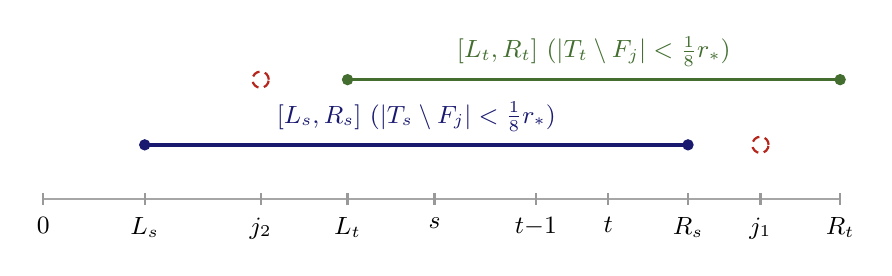
\begin{tikzpicture}[scale=0.92, every node/.style={font=\small}]
  % Axis 0 .. \ell
  \draw[thick, gray!70] (0, 0) -- (11, 0);
  \foreach \x in {0, 1.4, 3.0, 4.2, 5.4, 6.8, 7.8, 8.9, 9.9, 11} {
    \draw[thick, gray!80] (\x, -0.08) -- (\x, 0.08);
  }
  \node[below] at (0, -0.12) {$0$};
  \node[below] at (1.4, -0.12) {$L_s$};
  \node[below] at (3.0, -0.12) {$j_2$};
  \node[below] at (4.2, -0.12) {$L_t$};
  \node[below] at (5.4, -0.12) {$s$};
  \node[below] at (6.8, -0.12) {$t{-}1$};
  \node[below] at (7.8, -0.12) {$t$};
  \node[below] at (8.9, -0.12) {$R_s$};
  \node[below] at (9.9, -0.12) {$j_1$};
  \node[below] at (11, -0.12) {$R_t$};

  % Interval [L_s, R_s]
  \draw[very thick, MidnightBlue] (1.4, 0.75) -- (8.9, 0.75);
  \filldraw[MidnightBlue] (1.4, 0.75) circle (2pt);
  \filldraw[MidnightBlue] (8.9, 0.75) circle (2pt);
  \node[MidnightBlue, above] at (5.15, 0.8) {$[L_s, R_s]$ ($|T_s \setminus F_j| < \frac{1}{8} r_*$)};
  \draw[BrickRed, thick, densely dashed] (9.9, 0.75) circle (3.2pt);

  % Interval [L_t, R_t]
  \draw[very thick, OliveGreen!80!black] (4.2, 1.65) -- (11, 1.65);
  \filldraw[OliveGreen!80!black] (4.2, 1.65) circle (2pt);
  \filldraw[OliveGreen!80!black] (11, 1.65) circle (2pt);
  \node[OliveGreen!80!black, above] at (7.6, 1.7) {$[L_t, R_t]$ ($|T_t \setminus F_j| < \frac{1}{8} r_*$)};
  \draw[BrickRed, thick, densely dashed] (3.0, 1.65) circle (3.2pt);
\end{tikzpicture}
\caption{The two crossing intervals provided by Lemma~\ref{lem:interval-crossing}: for $j_1 = R_s + 1$ we have $|T_s \setminus F_{j_1}| \ge \frac{1}{8} r_*$, while both $s$ and $j_1$ lie inside $[L_t, R_t]$ (forcing $|T_t| < |T_s|$); for $j_2 = L_t - 1$ we have $|T_t \setminus F_{j_2}| \ge \frac{1}{8} r_*$, while both $j_2$ and $t - 1$ lie inside $[L_s, R_s]$ (forcing $|T_s| < |T_t|$).}
\label{fig:interval-crossing}
\end{figure}

\begin{proof}[Proof of Theorem~\ref{thm:mod2-combinatorial}(b)]
At a fixed step $s \in \{1, \dots, \ell\}$, write $W_s := F_{s-1} \cup F_s$. We try to chip away $F_{s-1} \cap F_s$ one piece $A_r$ at a time using sets $F_{t_r}$ from the sequence, requiring each step to peel off at least $\frac{1}{8} r_*$ elements while picking up nearly as many elements of $W_s$ outside the unpeeled remainder. Formally, call a sequence $(t_1, \dots, t_k)$ of indices in $[0, \ell]$ ($k \ge 0$) an \emph{$s$-valid peeling} if, setting $I_0 := F_{s-1} \cap F_s$ and inductively $A_r := I_{r-1} \setminus F_{t_r}$ and $I_r := I_{r-1} \cap F_{t_r}$ for $1 \le r \le k$, every $1 \le r \le k$ satisfies
\[
|A_r| \;\ge\; \frac{1}{8}\,r_* \qquad \text{and} \qquad \bigl|(W_s \cap F_{t_r}) \setminus I_{r-1}\bigr| \;\ge\; |A_r| - \frac{1}{4}\,r_*.
\]
By construction, $I_{r-1} = A_r \sqcup I_r$ ($1 \le r \le k$), so $A_1, \dots, A_k, I_k$ partition $F_{s-1} \cap F_s$ into pairwise disjoint sets with $I_{r-1} = A_r \sqcup \dots \sqcup A_k \sqcup I_k$, $A_r \cap F_{t_r} = \emptyset$, and $I_r \subseteq F_{t_r}$. Moreover, $\frac{k}{8} r_* \le \sum_{r=1}^k |A_r| \le |F_{s-1} \cap F_s| \le |F_s| \le C_1 r_*$, so every $s$-valid peeling has length $0 \le k \le 8 C_1 = k_{\max}$.

Because the empty sequence ($k = 0$, $I_0 = F_{s-1} \cap F_s$) is vacuously $s$-valid and $|I_k| \in \{0, \dots, |F_{s-1} \cap F_s|\}$, we may fix for each $s \in \{1, \dots, \ell\}$ an $s$-valid peeling that minimizes the final remainder size $|I_k|$, and denote its final remainder by $T_s := I_k \subseteq F_{s-1} \cap F_s \subseteq W_s$. By minimality of $|T_s|$, no index $j \in [0, \ell]$ can be appended to this peeling; since $|T_s \cap F_j| < |T_s|$ whenever $|T_s \setminus F_j| \ge \frac{1}{8} r_* > 0$, every $j \in [0, \ell]$ with $|T_s \setminus F_j| \ge \frac{1}{8} r_*$ must violate the second condition, meaning $|(W_s \cap F_j) \setminus T_s| < |T_s \setminus F_j| - \frac{1}{4} r_*$. Adding $|(W_s \cap F_j) \cap T_s| = |T_s \cap F_j|$ to both sides yields, for every $j \in [0, \ell]$,
\begin{equation}
\label{eq:greedy-stability}
|T_s \setminus F_j| \;\ge\; \frac{1}{8}\,r_* \qquad \Longrightarrow \qquad |W_s \cap F_j| \;<\; |T_s| - \frac{1}{4}\,r_*.
\end{equation}

If $|T_s| \le \frac{1}{2} r_*$ for some $s \in \{1, \dots, \ell\}$, then the chosen $s$-valid peeling satisfies all conclusions of Theorem~\ref{thm:mod2-combinatorial}(b). Suppose for contradiction that $|T_s| > \frac{1}{2} r_*$ for every $s \in \{1, \dots, \ell\}$. Since $T_s \subseteq F_{s-1} \cap F_s$, we have $|T_s \setminus F_{s-1}| = |T_s \setminus F_s| = 0 < \frac{1}{8} r_*$. Define
\begin{align*}
L_s &\;:=\; \min\bigl\{a \in [0, s - 1] : \forall j \in [a, s - 1],\, |T_s \setminus F_j| < \tfrac{1}{8} r_*\bigr\}, \\
R_s &\;:=\; \max\bigl\{b \in [s, \ell] : \forall j \in [s, b],\, |T_s \setminus F_j| < \tfrac{1}{8} r_*\bigr\}.
\end{align*}
Then $0 \le L_s \le s - 1 < s \le R_s \le \ell$, and $|T_s \setminus F_j| < \frac{1}{8} r_*$ for all $j \in [L_s, R_s]$. Also, $(L_s, R_s) \ne (0, \ell)$: if $(L_s, R_s) = (0, \ell)$, then $|T_s \setminus F_0| < \frac{1}{8} r_*$ and $|T_s \setminus F_\ell| < \frac{1}{8} r_*$, giving
\[
|F_0 \cap F_\ell| \;\ge\; |T_s \cap F_0 \cap F_\ell| \;\ge\; |T_s| - |T_s \setminus F_0| - |T_s \setminus F_\ell| \;>\; \left(\frac{1}{2} - \frac{2}{8}\right) r_* \;=\; \frac{1}{4}\,r_*,
\]
contradicting $|F_0 \cap F_\ell| \le \frac{1}{4} r_*$.

Applying Lemma~\ref{lem:interval-crossing} on $[\alpha, \beta] = [1, \ell]$ produces $1 \le s < t \le \ell$ with $L_s < L_t \le s < t \le R_s + 1 \le R_t$ (Figure~\ref{fig:interval-crossing}):
\begin{itemize}[leftmargin=2em,nosep]
  \item Set $j_1 := R_s + 1 \le R_t \le \ell$. Maximality of $R_s$ gives $|T_s \setminus F_{j_1}| \ge \frac{1}{8} r_*$, so $|W_s \cap F_{j_1}| < |T_s| - \frac{1}{4} r_*$ by~\eqref{eq:greedy-stability}. Conversely, $L_t \le s < t \le j_1 \le R_t$ puts both $s$ and $j_1$ in $[L_t, R_t]$, so $|T_t \setminus F_s| < \frac{1}{8} r_*$ and $|T_t \setminus F_{j_1}| < \frac{1}{8} r_*$. Since $F_s \subseteq W_s$, we obtain $|W_s \cap F_{j_1}| \ge |T_t \cap F_s \cap F_{j_1}| > |T_t| - \frac{2}{8} r_* = |T_t| - \frac{1}{4} r_*$, whence $|T_t| < |T_s|$.
  \item Symmetrically, set $j_2 := L_t - 1 \ge L_s \ge 0$. Minimality of $L_t$ gives $|T_t \setminus F_{j_2}| \ge \frac{1}{8} r_*$, so $|W_t \cap F_{j_2}| < |T_t| - \frac{1}{4} r_*$ by~\eqref{eq:greedy-stability}. Meanwhile, $L_s \le j_2 < s \le t - 1 \le R_s$ puts both $j_2$ and $t - 1$ in $[L_s, R_s]$, so $|T_s \setminus F_{j_2}| < \frac{1}{8} r_*$ and $|T_s \setminus F_{t-1}| < \frac{1}{8} r_*$. Since $F_{t-1} \subseteq W_t$, we have $|W_t \cap F_{j_2}| \ge |T_s \cap F_{t-1} \cap F_{j_2}| > |T_s| - \frac{1}{4} r_*$, whence $|T_s| < |T_t|$.
\end{itemize}
The inequalities $|T_t| < |T_s|$ and $|T_s| < |T_t|$ contradict each other, completing the proof.
\end{proof}


% ============================================================================
\section{Proof of Step 3: Hard Codes from Random Constraint Satisfaction Problems}
\label{sec:csp-cloud}
% ============================================================================

This section proves Theorem~\ref{thm:mod3-cloud}. The code $\mathcal{X}$ is obtained from the set of satisfying assignments of a random constraint satisfaction problem with one constraint for every pair of coordinates, by random sampling followed by the deletion of a small number of bad points; the analysis uses the second-moment and deletion methods~\cite{alon2016probabilistic}. Section~\ref{subsec:csp-lists} defines the lists and shows, by a deterministic argument based on Theorem~\ref{thm:mod2-combinatorial}(b), that they satisfy Condition~\textbf{(List-Hit)} (Lemma~\ref{lem:list-hit}). Section~\ref{subsec:csp-moment} fixes the parameters of the random model and bounds the moments of the list sizes (Lemma~\ref{lem:list-moment}). Section~\ref{subsec:second-moment} bounds the second moments of the number of close pairs (Lemma~\ref{lem:second-moment}), and Section~\ref{subsec:deletion} combines these ingredients.

\subsection{Constraint Systems and the Definition of the Lists}
\label{subsec:csp-lists}

\begin{definition*}[Constraint Systems, Three-Way Disagreements, and Alternative Colors]
We build codes from strings in $[q]^N$ (whose alphabet elements we call \emph{colors}) that satisfy a pairwise constraint on every pair of coordinates. To compare a candidate origin $x$ with an edge $(a, b)$ and another codeword $z$, we also record where three strings take three distinct colors and pick out, on every coordinate where $a$ or $b$ differs from $x$, a single color from $\{a_v, b_v\} \setminus \{x_v\}$:
\begin{itemize}[leftmargin=2em,nosep,topsep=4pt,itemsep=3pt]
  \item \textbf{Constraint systems and satisfying assignments.} Fix integers $N, q \ge 2$. A \emph{constraint system} $R = (R_{u, v})_{1 \le u < v \le N}$ over $[q]$ assigns a relation $R_{u, v} \subseteq [q] \times [q]$ of allowed color pairs to each coordinate pair $1 \le u < v \le N$; for $1 \le v < u \le N$, we write $R_{u, v} := \{(c_2, c_1) : (c_1, c_2) \in R_{v, u}\}$. Thus for every ordered pair of distinct coordinates $(u, v) \in [N]^2$ and colors $(c_1, c_2) \in [q]^2$, membership $(c_1, c_2) \in R_{u, v}$ depends only on the \emph{canonical entry}
  \[
  \mathrm{entry}(u, c_1;\, v, c_2) \;:=\;
  \begin{cases}
  (u, v, c_1, c_2) & \text{if } u < v, \\
  (v, u, c_2, c_1) & \text{if } u > v.
  \end{cases}
  \]
  The set of \emph{satisfying assignments} of $R$ is $\Omega(R) := \bigl\{x \in [q]^N : \forall 1 \le u < v \le N,\; (x_u, x_v) \in R_{u, v}\bigr\}$.
  \item \textbf{Three-way disagreement set.} For three strings $x, y, z \in [q]^N$, their \emph{three-way disagreement set} is the set of coordinates where all three colors are pairwise distinct:
  \[
  D_3(x, y, z) \;:=\; \bigl\{v \in [N] : |\{x_v, y_v, z_v\}| = 3\bigr\} \;\subseteq\; \Delta(x, y) \cap \Delta(x, z).
  \]
  \item \textbf{Disagreement window and alternative color.} Given $x, a, b \in [q]^N$, let $W(x, a, b) := \Delta(x, a) \cup \Delta(x, b)$ be the set of coordinates where at least one of $a$ or $b$ differs from $x$. For each $v \in W(x, a, b)$, define the \emph{alternative color} (preferring $a_v$ when $a_v \ne x_v$) by
  \[
  c_v(x, a, b) \;:=\;
  \begin{cases}
  a_v & \text{if } a_v \ne x_v, \\
  b_v & \text{if } a_v = x_v.
  \end{cases}
  \]
\end{itemize}
\end{definition*}

Because $v \in \Delta(x, a) \cup \Delta(x, b)$, if $a_v = x_v$ then $b_v \ne x_v$; hence $c_v(x, a, b) \in \{a_v, b_v\} \setminus \{x_v\}$ and $c_v(x, a, b) \ne x_v$ for every $v \in W(x, a, b)$. In addition, if a fourth string $z \in [q]^N$ differs from $x$ at $v \in \bigl(W(x, a, b) \cap \Delta(x, z)\bigr) \setminus \bigl(D_3(x, a, z) \cup D_3(x, b, z)\bigr)$ without creating a three-way disagreement, then $z_v$ must equal $c_v(x, a, b)$: indeed, $z_v \ne x_v$, so if $v \in \Delta(x, a)$ then $a_v \ne x_v$ and $|\{x_v, a_v, z_v\}| \le 2$ force $z_v = a_v = c_v(x, a, b)$, whereas if $v \in \Delta(x, b) \setminus \Delta(x, a)$ then $a_v = x_v$, $b_v \ne x_v$, and $|\{x_v, b_v, z_v\}| \le 2$ force $z_v = b_v = c_v(x, a, b)$.

\begin{definition}[The Lists $\mathcal{L}_R(a, b)$]
\label{def:witness-list}
Given a short step $(a, b)$ between two satisfying assignments, the list $\mathcal{L}_R(a, b)$ collects all nearby satisfying assignments $x \notin \{a, b\}$ whose shared disagreement set $\Delta(x, a) \cap \Delta(x, b)$ can be peeled away in at most $k_{\max} = 8 C_1$ disjoint pieces $A_1, \dots, A_k$ down to a remainder $I_k$ of size at most $\frac{1}{2} r_*$, such that every piece $A_r$ sends a dense biclique of \emph{hybrid constraints}---pairing $x$'s colors on $A_r$ with the alternative colors $c_v(x, a, b) \in \{a_v, b_v\} \setminus \{x_v\}$---both into nearly all of the unpeeled remainder $I_r$ and into nearly $|A_r| - \frac{1}{4} r_*$ coordinates of $W(x, a, b)$ outside $A_r \cup I_r$ (Figure~\ref{fig:hybrid-biclique}).

Formally, let $C_1 \ge 3$ and $r_* \ge 1$ be integers, and recall $k_{\max} = 8 C_1$. For $(a, b) \in \Omega(R)^2$ with $0 < \dHam(a, b) \le C_1 r_*$, define $\mathcal{L}_R(a, b)$ to be the set of all $x \in \Omega(R) \setminus \{a, b\}$ satisfying $\dHam(x, a) \le C_1 r_*$ and $\dHam(x, b) \le C_1 r_*$ for which there exist:
\begin{itemize}[leftmargin=2em,nosep,topsep=3pt,itemsep=2pt]
  \item an integer $0 \le k \le k_{\max}$ and pairwise disjoint subsets $A_1, \dots, A_k, I_k \subseteq \Delta(x, a) \cap \Delta(x, b)$ with $\Delta(x, a) \cap \Delta(x, b) = A_1 \sqcup \dots \sqcup A_k \sqcup I_k$ and $|I_k| \le \frac{1}{2} r_*$ (write $I_{r-1} := A_r \sqcup \dots \sqcup A_k \sqcup I_k$ for $1 \le r \le k + 1$); and
  \item for each $1 \le r \le k$, subsets $B_r^{\mathrm{fut}} \subseteq I_r$ and $B_r^{\mathrm{out}} \subseteq W(x, a, b) \setminus I_{r-1}$,
\end{itemize}
such that every $1 \le r \le k$ satisfies:
\begin{enumerate}[label=(\arabic*),leftmargin=2em,nosep,topsep=3pt,itemsep=2pt]
  \item \emph{(Hybrid constraints.)} $(x_u, c_v(x, a, b)) \in R_{u, v}$ for all $u \in A_r$ and $v \in B_r^{\mathrm{fut}} \cup B_r^{\mathrm{out}}$ (note $u \ne v$ since $A_r$, $I_r$, and $W(x, a, b) \setminus I_{r-1}$ are pairwise disjoint); and
  \item \emph{(Biclique sizes.)} $|I_r \setminus B_r^{\mathrm{fut}}| \le \frac{1}{80} r_*$ and $|B_r^{\mathrm{out}}| \ge |A_r| - \frac{11}{40} r_*$.
\end{enumerate}
\end{definition}

\begin{figure}[ht]
\centering
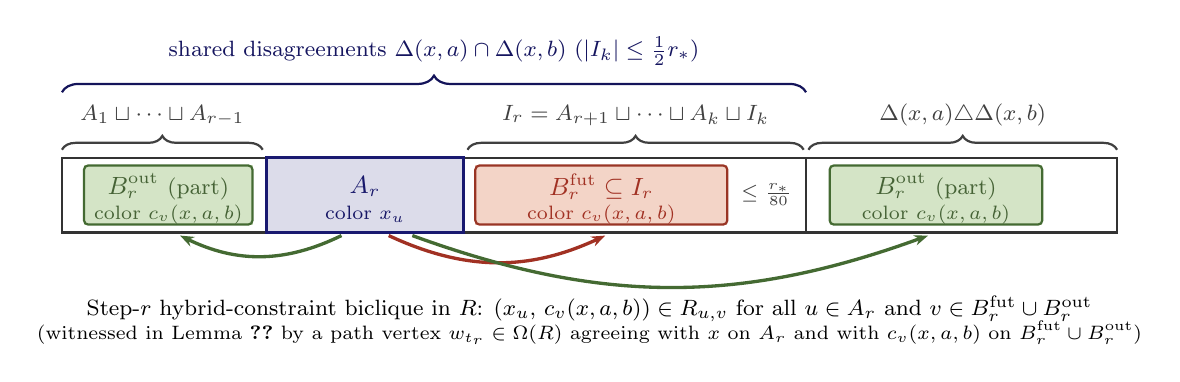
\begin{tikzpicture}[every node/.style={font=\small}, >={Stealth[length=5pt]}]
  % Main coordinate strip W(x, a, b) = \Delta(x, a) \cup \Delta(x, b) from x=0 to x=13.4, y=0 to y=0.95
  % Sub-highlights first
  % B_r^{out} part 1 inside A_1 \sqcup ... \sqcup A_{r-1}
  \fill[OliveGreen!18] (0.28, 0.1) rectangle (2.42, 0.85);
  \draw[OliveGreen!75!black, thick, rounded corners=1.5pt] (0.28, 0.1) rectangle (2.42, 0.85);
  % A_r
  \fill[MidnightBlue!15] (2.6, 0) rectangle (5.1, 0.95);
  % B_r^{fut} inside I_r
  \fill[BrickRed!15] (5.25, 0.1) rectangle (8.45, 0.85);
  \draw[BrickRed!80!black, thick, rounded corners=1.5pt] (5.25, 0.1) rectangle (8.45, 0.85);
  % B_r^{out} part 2 inside \Delta(x, a) \triangle \Delta(x, b)
  \fill[OliveGreen!18] (9.75, 0.1) rectangle (12.45, 0.85);
  \draw[OliveGreen!75!black, thick, rounded corners=1.5pt] (9.75, 0.1) rectangle (12.45, 0.85);

  % Outer frame and dividers
  \draw[thick, black!80] (0, 0) rectangle (13.4, 0.95);
  \draw[very thick, MidnightBlue] (2.6, 0) rectangle (5.1, 0.95);
  \draw[thick, black!80] (9.45, 0) -- (9.45, 0.95);

  % Block labels inside strip
  \node[OliveGreen!65!black] at (1.35, 0.58) {\textbf{$B_r^{\mathrm{out}}$} {\footnotesize (part)}};
  \node[OliveGreen!65!black, font=\scriptsize] at (1.35, 0.23) {color $c_v(x, a, b)$};
  \node[MidnightBlue!95!black] at (3.85, 0.58) {\textbf{$A_r$}};
  \node[MidnightBlue!90!black, font=\scriptsize] at (3.85, 0.23) {color $x_u$};
  \node[BrickRed!85!black] at (6.85, 0.58) {\textbf{$B_r^{\mathrm{fut}} \subseteq I_r$}};
  \node[BrickRed!85!black, font=\scriptsize] at (6.85, 0.23) {color $c_v(x, a, b)$};
  \node[black!75, font=\scriptsize] at (8.95, 0.48) {$\le \frac{r_*}{80}$};
  \node[OliveGreen!65!black] at (11.1, 0.58) {\textbf{$B_r^{\mathrm{out}}$} {\footnotesize (part)}};
  \node[OliveGreen!65!black, font=\scriptsize] at (11.1, 0.23) {color $c_v(x, a, b)$};

  % Top braces
  \draw[decorate, decoration={brace, amplitude=5pt}, thick, black!75] (0, 1.05) -- (2.55, 1.05)
    node[midway, above=5pt, font=\footnotesize] {$A_1 \sqcup \dots \sqcup A_{r-1}$};
  \draw[decorate, decoration={brace, amplitude=5pt}, thick, black!75] (5.15, 1.05) -- (9.42, 1.05)
    node[midway, above=5pt, font=\footnotesize] {$I_r = A_{r+1} \sqcup \dots \sqcup A_k \sqcup I_k$};
  \draw[decorate, decoration={brace, amplitude=5pt}, thick, black!75] (9.48, 1.05) -- (13.4, 1.05)
    node[midway, above=5pt, font=\footnotesize] {$\Delta(x, a) \triangle \Delta(x, b)$};
  \draw[decorate, decoration={brace, amplitude=6pt}, thick, MidnightBlue!80!black] (0, 1.78) -- (9.45, 1.78)
    node[midway, above=6pt, font=\footnotesize, text=MidnightBlue!85!black] {shared disagreements $\Delta(x, a) \cap \Delta(x, b)$ ($|I_k| \le \tfrac{1}{2} r_*$)};

  % Hybrid-constraint biclique arrows below the strip
  \draw[->, very thick, BrickRed!85!black] (4.15, -0.04) to[bend right=25] (6.9, -0.04);
  \draw[->, very thick, OliveGreen!75!black] (3.55, -0.04) to[bend left=26] (1.5, -0.04);
  \draw[->, very thick, OliveGreen!75!black] (4.45, -0.04) to[bend right=20] (11.0, -0.04);

  \node[align=center, font=\footnotesize] at (6.7, -1.12)
    {Step-$r$ hybrid-constraint biclique in $R$: $(x_u,\, c_v(x, a, b)) \in R_{u, v}$ for all $u \in A_r$ and $v \in B_r^{\mathrm{fut}} \cup B_r^{\mathrm{out}}$\\[-1pt]
    {\scriptsize (witnessed in Lemma~\ref{lem:list-hit} by a path vertex $w_{t_r} \in \Omega(R)$ agreeing with $x$ on $A_r$ and with $c_v(x, a, b)$ on $B_r^{\mathrm{fut}} \cup B_r^{\mathrm{out}}$)}};
\end{tikzpicture}
\caption{Step $r \in \{1, \dots, k\}$ of the peeling witness in Definition~\ref{def:witness-list} inside the disagreement window $W(x, a, b) = \Delta(x, a) \cup \Delta(x, b)$. The current piece $A_r$ sends hybrid constraints $(x_u, c_v(x, a, b)) \in R_{u, v}$ to $B_r^{\mathrm{fut}} \subseteq I_r$ (missing at most $\frac{1}{80} r_*$ coordinates of $I_r$) and to $B_r^{\mathrm{out}} \subseteq W(x, a, b) \setminus I_{r-1}$ (of size at least $|A_r| - \frac{11}{40} r_*$).}
\label{fig:hybrid-biclique}
\end{figure}

\begin{remark}[Why the Peeling Uses Few Disjoint Steps]
\label{rem:biclique-entropy}
Whereas standard list-decoding analyses of random and graph-based codes bound the number of codewords inside single-center Hamming balls~\cite{guruswami2002combinatorial,mosheiff2020ldpc}, Definition~\ref{def:witness-list} controls a list $\mathcal{L}_R(a, b)$ attached to a pair of codewords, that is, to a potential spanner edge. Partitioning $\Delta(x, a) \cap \Delta(x, b)$ into $k \le k_{\max} = 8 C_1$ pairwise disjoint pieces $A_1, \dots, A_k$ (besides $I_k$) serves two purposes in Lemma~\ref{lem:list-moment}: first, the losses $|I_r \setminus B_r^{\mathrm{fut}}| \le \frac{1}{80} r_*$ and $|A_r| - |B_r^{\mathrm{out}}| \le \frac{11}{40} r_*$ sum over $r \in [k]$ with weights $|M \cap A_r|$ that add up to at most $|M|$, without multiplying by $k$; second, restricting the witness to a set $M$ of $m$ fresh coordinates leaves at most $2^{O(C_1 m + r_*)}$ possible patterns, whereas arbitrary sets of coordinate pairs would cost $2^{\Theta(r_*^2)}$.
\end{remark}

\begin{lemma}[Verification of Condition~\textbf{(List-Hit)}]
\label{lem:list-hit}
Let $C_1 \ge 3$ and $r_* \ge 1$ be integers, and set $\eta_0 := \frac{1}{80}$. Suppose $\mathcal{X} \subseteq \Omega(R)$ satisfies $|D_3(x, u, z)| \le \eta_0 r_*$ for all $x, u \in \mathcal{X}$ and $z \in \Omega(R)$ with $\dHam(x, u) \le C_1 r_*$ and $\dHam(x, z) \le C_1 r_*$. Define $\mathcal{L}_{\mathcal{X}} : \mathcal{X}^2 \to 2^{\mathcal{X}}$ by $\mathcal{L}_{\mathcal{X}}(a, b) := \mathcal{L}_R(a, b) \cap \mathcal{X}$ when $0 < \dHam(a, b) \le C_1 r_*$ and $\mathcal{L}_{\mathcal{X}}(a, b) := \emptyset$ otherwise. Then $\mathcal{L}_{\mathcal{X}}$ satisfies Condition~\textbf{(List-Hit)} of Section~\ref{subsec:mod2} with parameters $C_1$ and $r_*$.
\end{lemma}

\begin{proof}
Let $x \in \mathcal{X}$ and $w_0, \dots, w_\ell \in B_{\mathcal{X}}(x, C_1 r_*) \setminus \{x\}$ ($\ell \ge 1$) satisfy $0 < \dHam(w_{s-1}, w_s) \le C_1 r_*$ ($1 \le s \le \ell$), $\dHam(x, w_\ell) = r_*$, and $|\Delta(x, w_0) \cap \Delta(x, w_\ell)| \le \frac{1}{4} r_*$. Put $F_t := \Delta(x, w_t) \subseteq [N]$ for $0 \le t \le \ell$, so $|F_t| \le C_1 r_*$, $|F_\ell| = r_*$, and $|F_0 \cap F_\ell| \le \frac{1}{4} r_*$. Theorem~\ref{thm:mod2-combinatorial}(b) yields $s \in \{1, \dots, \ell\}$, $0 \le k \le k_{\max}$, indices $t_1, \dots, t_k \in \{0, \dots, \ell\}$, and a partition $F_{s-1} \cap F_s = A_1 \sqcup \dots \sqcup A_k \sqcup I_k$ with $|I_k| \le \frac{1}{2} r_*$ such that, writing $I_{r-1} := A_r \sqcup \dots \sqcup A_k \sqcup I_k$ and $W_s := F_{s-1} \cup F_s$, every $1 \le r \le k$ satisfies
\begin{equation}
\label{eq:hit-pretrim}
A_r \cap F_{t_r} \;=\; \emptyset, \qquad I_r \;\subseteq\; F_{t_r}, \qquad \text{and} \qquad \bigl|(W_s \cap F_{t_r}) \setminus I_{r-1}\bigr| \;\ge\; |A_r| - \frac{1}{4}\,r_*.
\end{equation}
Set $(a, b) := (w_{s-1}, w_s) \in \mathcal{X}^2 \subseteq \Omega(R)^2$. Then $0 < \dHam(a, b) \le C_1 r_*$, $x \in \mathcal{X} \setminus \{a, b\}$, $\dHam(x, a) \le C_1 r_*$, $\dHam(x, b) \le C_1 r_*$, $\Delta(x, a) \cap \Delta(x, b) = F_{s-1} \cap F_s$, and also $W(x, a, b) = W_s$. For each $1 \le r \le k$, define
\begin{align*}
B_r^{\mathrm{fut}} &\;:=\; I_r \setminus D_3(x, a, w_{t_r}), \\
B_r^{\mathrm{out}} &\;:=\; \bigl((W_s \cap F_{t_r}) \setminus I_{r-1}\bigr) \setminus \bigl(D_3(x, a, w_{t_r}) \cup D_3(x, b, w_{t_r})\bigr).
\end{align*}
Then $B_r^{\mathrm{fut}} \subseteq I_r$ and $B_r^{\mathrm{out}} \subseteq W(x, a, b) \setminus I_{r-1}$. Because $I_r \subseteq (F_{s-1} \cap F_s) \cap F_{t_r} \subseteq \Delta(x, a) \cap \Delta(x, w_{t_r})$, every $v \in B_r^{\mathrm{fut}}$ satisfies $a_v \ne x_v$, $(w_{t_r})_v \ne x_v$, and $|\{x_v, a_v, (w_{t_r})_v\}| \le 2$, forcing $(w_{t_r})_v = a_v = c_v(x, a, b)$; likewise $(w_{t_r})_v = c_v(x, a, b)$ for every $v \in B_r^{\mathrm{out}}$ by the observation preceding Definition~\ref{def:witness-list}. Meanwhile, every $u \in A_r$ satisfies $u \notin F_{t_r} = \Delta(x, w_{t_r})$, so $(w_{t_r})_u = x_u$. Since $w_{t_r} \in \mathcal{X} \subseteq \Omega(R)$ and $A_r \cap (B_r^{\mathrm{fut}} \cup B_r^{\mathrm{out}}) = \emptyset$, we obtain $(x_u, c_v(x, a, b)) = ((w_{t_r})_u, (w_{t_r})_v) \in R_{u, v}$ for all $u \in A_r$ and $v \in B_r^{\mathrm{fut}} \cup B_r^{\mathrm{out}}$, verifying item~(1) of Definition~\ref{def:witness-list}.

For item~(2), since $x, a, b \in \mathcal{X}$ and $w_{t_r} \in \mathcal{X} \subseteq \Omega(R)$ all lie within Hamming distance $C_1 r_*$ of $x$, the hypothesis gives $|D_3(x, a, w_{t_r})| \le \eta_0 r_* = \frac{1}{80} r_*$ and $|D_3(x, b, w_{t_r})| \le \frac{1}{80} r_*$. Hence $|I_r \setminus B_r^{\mathrm{fut}}| \le |D_3(x, a, w_{t_r})| \le \frac{1}{80} r_*$, and~\eqref{eq:hit-pretrim} yields $|B_r^{\mathrm{out}}| \ge |A_r| - \frac{1}{4} r_* - \frac{2}{80} r_* = |A_r| - \frac{11}{40} r_*$. Thus $x \in \mathcal{L}_R(a, b) \cap \mathcal{X} = \mathcal{L}_{\mathcal{X}}(w_{s-1}, w_s)$.
\end{proof}

\subsection{The Random Model and the Moments of the List Sizes}
\label{subsec:csp-moment}

Fix an integer $C_1 \ge 3$ for the remainder of Section~\ref{sec:csp-cloud}, and define the integer constants (together with $\eta_0 := \frac{1}{80}$ and $c(C_1)$)
\begin{align*}
K &\;:=\; 20 C_1^2, & \lambda_0 &\;:=\; 100 C_1\bigl(2\lceil \log_2 C_1 \rceil + 6\bigr), & \beta_0 &\;:=\; 6 \lambda_0, & \gamma_0 &\;:=\; 5 \lambda_0, \\
L &\;:=\; 1600 C_1^2 \lambda_0 + 20, & E_q &\;:=\; 2 \beta_0 2^L, & q &\;:=\; 2^{E_q} + 1, & R_0 &\;:=\; 1000 C_1 + 1, \\
\mu_0 &\;:=\; \beta_0 2^{2 L}, & c(C_1) &\;:=\; 2^{-(2 L + 5)}.
\end{align*}
Here $K$ is the list-size threshold, $\beta_0 > \gamma_0$ control the quadratic constraint-sharing surplus versus the linear per-coordinate penalty (in units of $\lambda_0$), $2^L = N/r_*$ is the ratio of block length to close-pair distance, $q = 2^{E_q} + 1$ is the alphabet size, and $c(C_1)$ is the resulting spanner-size exponent. Since $C_1 \ge 3$, we have $\lceil \log_2 C_1 \rceil \ge 2$, $K \ge 180$, $\lambda_0 \ge 1000 C_1 \ge 3000$ with $\lambda_0 = \Theta(C_1 \log C_1)$, $\eta_0 L = 20 C_1^2 \lambda_0 + \frac{1}{4} > 20 C_1^2 \lambda_0$, $L = \Theta(C_1^3 \log C_1)$ with $L > 4 \times 10^7$, $q - 1 = 2^{E_q} > 2^{10^8}$, and $R_0 = 1000 C_1 + 1 > \max(3000, 160 C_1)$; moreover, since $21 e < 64 = 2^6$, we have $21 e C_1^2 < 2^{2\lceil \log_2 C_1 \rceil + 6}$ and hence $C_1 \log_2(21 e C_1^2) < 0.01 \lambda_0$. By Stirling's inequality~\cite{robbins1955remark}, $(s/e)^s < s! \le e s (s/e)^s$ for every integer $s \ge 1$. Using $\sup_{t > 0} (1/t)^t = e^{1/e} < 2^{0.54}$ and $\sup_{t > 0} (e/t)^t = e < 2^{1.45}$ (with $0^0 := 1$), every integer $s \ge 0$ satisfies $(r_*/s)^s \le 2^{0.54 r_*}$ and $(e r_*/s)^s \le 2^{1.45 r_*}$, whence $\binom{U}{s} \le A^s 2^{1.45 r_*}$ for all integers $A \ge 1$ and $0 \le U \le A r_*$ (vanishing if $s > U$, and bounded by $\frac{(A r_*)^s}{s!} \le A^s (e r_*/s)^s$ for $1 \le s \le U$). Also, since $\frac{d}{dx}\bigl[x\ln(e M_{\mathrm{pool}}/x)\bigr] = \ln(e M_{\mathrm{pool}}/x) - 1 = \ln(M_{\mathrm{pool}}/x) \ge 0$ on $(0, M_{\mathrm{pool}}]$, any integers $1 \le b \le M_{\mathrm{pool}}$ and $0 \le U \le M_{\mathrm{pool}}$ satisfy $\sum_{s=0}^b \binom{U}{s} \le \sum_{s=0}^b \binom{M_{\mathrm{pool}}}{s} \le (b + 1)(e M_{\mathrm{pool}}/b)^b$.

Now fix any integer $r_* \ge R_0$, and set
\[
N \;:=\; 2^L r_*, \qquad \sigma_{\mathrm{edge}} \;:=\; \frac{E_q + L + \gamma_0 + 2}{N - 1}, \qquad p_{\mathrm{edge}} \;:=\; 2^{-\sigma_{\mathrm{edge}}} \in (0, 1).
\]
Since $q - 1 = 2^{E_q}$ and $e < 4 = 2^2$, the definition of $\sigma_{\mathrm{edge}}$ gives the exact identity
\begin{equation}
\label{eq:exact-calibration}
4 \cdot 2^L (q - 1)\,2^{-\sigma_{\mathrm{edge}}(N - 1)} \;=\; 2^{-\gamma_0}, \qquad \text{and hence} \qquad (e \cdot 2^L)(q - 1)\,2^{-\sigma_{\mathrm{edge}}(N - 1)} \;=\; \frac{e}{4}\,2^{-\gamma_0} \;<\; 2^{-\gamma_0}.
\end{equation}
Also, since $E_q = 2 \beta_0 2^L$, $r_* \ge 3001$, and $2^L - 1 \ge L^2 > 10^4 C_1^2 (2\beta_0 + L + \gamma_0 + 2)$, we have
\begin{equation}
\label{eq:sigma-window}
\beta_0 \;<\; \frac{\sigma_{\mathrm{edge}} r_*}{2} \;=\; \frac{2\beta_0 2^L + L + \gamma_0 + 2}{2(2^L - r_*^{-1})} \;\le\; \beta_0 + \frac{2\beta_0 + L + \gamma_0 + 2}{2(2^L - 1)} \;<\; \left(1 + \frac{1}{10^4 C_1^2}\right)\beta_0 \;\le\; 1.0001\,\beta_0.
\end{equation}

\begin{definition*}[Random $2$-CSP and Sampled Code]
We generate a random subset of $[q]^N$ in two stages: first we draw a permissive random pairwise constraint system, and then we independently subsample its satisfying assignments to eliminate too-close pairs while preserving many pairs at distance $r_*$:
\begin{itemize}[leftmargin=2em,nosep,topsep=4pt,itemsep=3pt]
  \item \textbf{Random constraint system $R$ and solution set $\Omega$.} Sample $R = (R_{u, v})_{1 \le u < v \le N}$ by including each ordered color pair $(c_1, c_2) \in [q]^2$ in $R_{u, v}$ independently with probability $p_{\mathrm{edge}} = 2^{-\sigma_{\mathrm{edge}}}$ (the complete-graph case of random binary CSP Model~A~\cite{achlioptas2001random,molloy2003models,frieze2006satisfiability}, taken here at constant alphabet $q = O_{C_1}(1)$ and vanishing tightness $1 - p_{\mathrm{edge}} = \Theta_{C_1}(1/N)$ well inside the satisfiable regime), and write $\Omega := \Omega(R)$ for its set of satisfying assignments.
  \item \textbf{Subsampled code $P_{\mathrm{raw}}$ and close pairs $E_{\mathrm{raw}}$.} Independently of $R$, draw independent Bernoulli coins $\xi_x \sim \Ber(p_{\mathrm{keep}})$ for all $x \in [q]^N$ (with $p_{\mathrm{keep}} \in (0, 1)$ calibrated below), and define the raw sampled code and its close pairs by
  \[
  P_{\mathrm{raw}} \;:=\; \{x \in \Omega : \xi_x = 1\} \quad \text{and} \quad E_{\mathrm{raw}} \;:=\; E_{r_*}(P_{\mathrm{raw}}) \;=\; \{(x, y) \in P_{\mathrm{raw}}^2 : \dHam(x, y) = r_*\}.
  \]
\end{itemize}
\end{definition*}

\paragraph{First-moment calibration.}
Each $x \in [q]^N$ satisfies $\Pr[x \in \Omega] = p_{\mathrm{edge}}^{\binom{N}{2}} = 2^{-\sigma_{\mathrm{edge}} N(N - 1)/2}$, so $\mathbb{E}[|\Omega|] = q^N 2^{-\sigma_{\mathrm{edge}} N(N - 1)/2}$. Conditioned on $x \in \Omega$, any $y \in [q]^N$ at distance $\dHam(x, y) = s \in \{1, \dots, N\}$ queries $s(N - s) + \binom{s}{2} = s(N - 1) - \binom{s}{2}$ canonical entries of $R$ disjoint from those of $x$ (one on every pair $\{u, v\}$ meeting $\Delta(x, y)$, since $y_u \ne x_u$ for $u \in \Delta(x, y)$). Thus the conditional expected number of $y \in \Omega$ with $\dHam(x, y) = s$ is
\[
D_\Omega(s) \;:=\; \binom{N}{s} (q - 1)^s\,2^{-\sigma_{\mathrm{edge}}\bigl(s(N - 1) - \binom{s}{2}\bigr)}
\]
(with $D_\Omega(0) := 1$). Applying $\binom{N}{s} \le \frac{N^s}{s!} < \left(\frac{e \cdot 2^L r_*}{s}\right)^s$ and~\eqref{eq:exact-calibration} yields, for every $1 \le s \le N$,
\begin{equation}
\label{eq:d-omega-upper}
D_\Omega(s) \;\le\; \left(\frac{r_*}{s}\right)^s 2^{-\gamma_0 s + \sigma_{\mathrm{edge}} \binom{s}{2}}.
\end{equation}
At $s = r_*$, using $\binom{N}{r_*} \ge \frac{(N - r_*)^{r_*}}{r_*!} \ge \frac{(1 - 2^{-L})^{r_*}}{e r_*} \left(\frac{e N}{r_*}\right)^{r_*}$ alongside $\log_2(e/4) > -0.56$, $\log_2(1 - 2^{-L}) \ge -3 \cdot 2^{-L}$, $\log_2(e r_*) < 0.01 r_*$ (as $r_* \ge 3001$), $r_* - 1 \ge \frac{3000}{3001} r_*$, $\beta_0 - \gamma_0 = \lambda_0$ ($\beta_0 = 6\lambda_0$, $\gamma_0 = 5\lambda_0$),~\eqref{eq:exact-calibration}, and~\eqref{eq:sigma-window} gives
\[
2^{0.997 \lambda_0 r_*} \;\le\; \frac{\bigl(\frac{e}{4}(1 - 2^{-L})\bigr)^{r_*}}{e r_*}\,2^{-\gamma_0 r_* + \sigma_{\mathrm{edge}} \binom{r_*}{2}} \;\le\; D_\Omega(r_*) \;\le\; 2^{-\gamma_0 r_* + \sigma_{\mathrm{edge}} \binom{r_*}{2}} \;\le\; 2^{1.001 \lambda_0 r_*}.
\]
Set $D_* := 2^{\frac{1}{4}\lambda_0 r_*}$ and $p_{\mathrm{keep}} := D_* / D_\Omega(r_*)$, so that $p_{\mathrm{keep}} \in (0, 1)$ satisfies
\begin{equation}
\label{eq:p-keep-bounds}
2^{-0.751 \lambda_0 r_*} \;\le\; p_{\mathrm{keep}} \;\le\; 2^{-0.747 \lambda_0 r_*}.
\end{equation}
Put $n_0 := \mathbb{E}[|P_{\mathrm{raw}}|] = p_{\mathrm{keep}}\mathbb{E}[|\Omega|]$ and $M_0 := \mathbb{E}[|E_{\mathrm{raw}}|] = p_{\mathrm{keep}}^2 \mathbb{E}[|\Omega|] D_\Omega(r_*) = n_0 D_*$. Since $\log_2 \mathbb{E}[|\Omega|] = N \log_2 q - \frac{N}{2}\bigl(E_q + L + \gamma_0 + 2\bigr)$ with $E_q = 2\beta_0 2^L < \log_2 q < E_q + 1$, we have $\log_2 \mathbb{E}[|\Omega|] \in [0.995 \mu_0 r_*, 1.005 \mu_0 r_*]$ ($\mu_0 = \beta_0 2^{2 L}$), and $|\log_2 p_{\mathrm{keep}}| \le \lambda_0 r_* < 2^{-2 L}\mu_0 r_*$ gives
\begin{equation}
\label{eq:n0-window}
0.99\,\mu_0 r_* \;\le\; \log_2 n_0 \;\le\; 1.01\,\mu_0 r_*.
\end{equation}
In addition, for every $1 \le s \le C_1 r_*$, convexity of $t \mapsto -5 t + 6\bigl(1 + \frac{1}{10^4 C_1^2}\bigr) t^2$ on $[0, C_1]$ gives $-\gamma_0 s + \sigma_{\mathrm{edge}}\binom{s}{2} \le (6 C_1^2 - 5 C_1 + 10^{-3})\lambda_0 r_* \le (6 C_1^2 - 14)\lambda_0 r_*$, so~\eqref{eq:d-omega-upper}--\eqref{eq:p-keep-bounds} bound the conditional expected size of the punctured $C_1 r_*$-ball in $P_{\mathrm{raw}}$ given $x \in P_{\mathrm{raw}}$ by
\begin{equation}
\label{eq:ball-expectation}
\sum_{s=1}^{C_1 r_*} p_{\mathrm{keep}} D_\Omega(s) \;\le\; C_1 r_* \cdot 2^{0.54 r_* - 0.747 \lambda_0 r_* + (6 C_1^2 - 14)\lambda_0 r_*} \;\le\; 2^{6 C_1^2 \lambda_0 r_*}.
\end{equation}

\begin{lemma}[Moments of the List Sizes]
\label{lem:list-moment}
Fix any $(a, b) \in [q]^N \times [q]^N$ with $0 < \dHam(a, b) \le C_1 r_*$, and let $\mathcal{E}_{a, b} := \{a \in P_{\mathrm{raw}} \text{ and } b \in P_{\mathrm{raw}}\}$. Conditioned on $\mathcal{E}_{a, b}$, the expected number of ordered $K$-tuples $(x^{(1)}, \dots, x^{(K)})$ of pairwise distinct points in $\mathcal{L}_R(a, b) \cap P_{\mathrm{raw}}$ is at most $2^{-8 C_1^2 \lambda_0 r_*}$.
\end{lemma}

\begin{proof}
For $0 \le t \le K$, let $N_t$ be the number of ordered $t$-tuples $(x^{(1)}, \dots, x^{(t)})$ of pairwise distinct strings in $\mathcal{L}_R(a, b) \cap P_{\mathrm{raw}}$ (with $N_0 := 1$). We prove $\mathbb{E}[N_t \mid \mathcal{E}_{a, b}] \le 2^{-0.72 t \lambda_0 r_*}$ by induction on $t$; at $t = K = 20 C_1^2$, this gives $2^{-14.4 C_1^2 \lambda_0 r_*} \le 2^{-8 C_1^2 \lambda_0 r_*}$.

The base case $t = 0$ is trivial. For $1 \le t \le K$, fix any $(t - 1)$-tuple $(x^{(1)}, \dots, x^{(t-1)})$ of pairwise distinct strings in $[q]^N \setminus \{a, b\}$ with $\dHam(x^{(s)}, a), \dHam(x^{(s)}, b) \le C_1 r_*$ ($1 \le s \le t - 1$), and let $\mathcal{R}_{t-1} \subseteq [N] \times [q]$ be the set of all coordinate-color pairs $(v, z_v)$ appearing in $z \in S_{t-1} := \{a, b, x^{(1)}, \dots, x^{(t-1)}\}$. Let $\mathcal{F}_{t-1}$ be the $\sigma$-algebra generated by $(\xi_z)_{z \in S_{t-1}}$ and all canonical entries $\mathrm{entry}(u, c_1; v, c_2)$ of $R$ with both $(u, c_1), (v, c_2) \in \mathcal{R}_{t-1}$. The event $\mathcal{E}_{t-1} := \mathcal{E}_{a, b} \cap \{x^{(1)}, \dots, x^{(t-1)} \in \mathcal{L}_R(a, b) \cap P_{\mathrm{raw}}\}$ is $\mathcal{F}_{t-1}$-measurable, since for each $z \in \{x^{(1)}, \dots, x^{(t-1)}\}$ both $z \in \Omega(R)$ and item~(1) of Definition~\ref{def:witness-list} inspect only canonical entries whose endpoints lie in $\{(u, z_u), (v, a_v), (v, b_v) : u, v \in [N]\} \subseteq \mathcal{R}_{t-1}$. Writing $\mathrm{graph}(a) := \{(v, a_v) : v \in [N]\}$, we also have $|\mathcal{R}_{t-1} \setminus \mathrm{graph}(a)| \le \dHam(a, b) + \sum_{s=1}^{t-1} \dHam(a, x^{(s)}) \le t C_1 r_* \le K C_1 r_*$.

Consider any candidate $x \in [q]^N \setminus S_{t-1}$ with $\dHam(x, a), \dHam(x, b) \le C_1 r_*$. Partition $\Delta(x, a)$ into $V_{\mathrm{old}} := \{v \in \Delta(x, a) : (v, x_v) \in \mathcal{R}_{t-1}\}$ and $M := \{v \in \Delta(x, a) : (v, x_v) \notin \mathcal{R}_{t-1}\}$, and put $m := |M| \in \{0, \dots, C_1 r_*\}$. Every $u \in M$ satisfies $(u, b_u) \in \mathcal{R}_{t-1}$ and $(u, x_u) \notin \mathcal{R}_{t-1}$, so $x_u \ne b_u$ as well as $x_u \ne a_u$; hence $M \subseteq \Delta(x, a) \cap \Delta(x, b)$. Because constraints among coordinates in $V_{\mathrm{old}}$ may already have been exposed in $\mathcal{F}_{t-1}$, we extract fresh randomness by restricting a peeling witness of Definition~\ref{def:witness-list} to the unexposed coordinates $M$ on the left and trimming each outside set to an exact deterministic size $\hat{s}_r$. Formally, define a \emph{projected witness} for $x$ to be a tuple $\widehat{\mathcal{W}} = \bigl(k, (M_1, \dots, M_k, M_{\mathrm{tail}}), (\widehat{B}_r^{\mathrm{fut}}, \widehat{B}_r^{\mathrm{out}})_{r=1}^k\bigr)$ where $0 \le k \le k_{\max}$, $(M_1, \dots, M_k, M_{\mathrm{tail}})$ is an ordered partition of $M$ into pairwise disjoint sets with $|M_{\mathrm{tail}}| \le \frac{1}{2} r_*$, and (setting $a_r := |M_r|$, $\widetilde{I}_r := M_{r+1} \sqcup \dots \sqcup M_k \sqcup M_{\mathrm{tail}}$, and $\hat{s}_r := \max\bigl(0, a_r - \lfloor \frac{11}{40} r_* \rfloor\bigr)$) each $1 \le r \le k$ satisfies $\widehat{B}_r^{\mathrm{fut}} \subseteq \widetilde{I}_r$ with $|\widetilde{I}_r \setminus \widehat{B}_r^{\mathrm{fut}}| \le \frac{1}{80} r_*$, $\widehat{B}_r^{\mathrm{out}} \subseteq W(x, a, b) \setminus (M_r \sqcup \widetilde{I}_r)$ with $|\widehat{B}_r^{\mathrm{out}}| = \hat{s}_r$, and $(x_u, c_v(x, a, b)) \in R_{u, v}$ for all $u \in M_r$ and $v \in \widehat{B}_r^{\mathrm{fut}} \cup \widehat{B}_r^{\mathrm{out}}$. Any $x \in \mathcal{L}_R(a, b)$ admits a projected witness: given a witness $(k, A_1, \dots, A_k, I_k, (B_r^{\mathrm{fut}}, B_r^{\mathrm{out}})_{r=1}^k)$ from Definition~\ref{def:witness-list}, set $M_r := M \cap A_r$, $M_{\mathrm{tail}} := M \cap I_k$ ($|M_{\mathrm{tail}}| \le |I_k| \le \frac{1}{2} r_*$), and $\widehat{B}_r^{\mathrm{fut}} := M \cap B_r^{\mathrm{fut}} \subseteq M \cap I_r = \widetilde{I}_r$ ($|\widetilde{I}_r \setminus \widehat{B}_r^{\mathrm{fut}}| \le |I_r \setminus B_r^{\mathrm{fut}}| \le \frac{1}{80} r_*$); since $|B_r^{\mathrm{out}}| \ge |A_r| - \frac{11}{40} r_* \ge a_r - \frac{11}{40} r_*$ is an integer, $|B_r^{\mathrm{out}}| \ge \hat{s}_r$, so we may pick an arbitrary subset $\widehat{B}_r^{\mathrm{out}} \subseteq B_r^{\mathrm{out}} \subseteq W(x, a, b) \setminus I_{r-1} \subseteq W(x, a, b) \setminus (M_r \sqcup \widetilde{I}_r)$ of size $\hat{s}_r$.

For fixed $m \in \{0, \dots, C_1 r_*\}$, count the choices of $(x, \widehat{\mathcal{W}})$:
\begin{itemize}[leftmargin=2em,nosep]
  \item Choosing $\{(v, x_v) : v \in V_{\mathrm{old}}\} \subseteq \mathcal{R}_{t-1} \setminus \mathrm{graph}(a)$ of size at most $C_1 r_*$ from $|\mathcal{R}_{t-1} \setminus \mathrm{graph}(a)| \le K C_1 r_*$ has at most $\sum_{s=0}^{C_1 r_*} \binom{K C_1 r_*}{s} \le (C_1 r_* + 1)(e K)^{C_1 r_*} \le (C_1 r_* + 1)\,2^{0.01 \lambda_0 r_*}$ options;
  \item Choosing $M \subseteq [N]$ of size $m$ and colors $x_u \in [q] \setminus \{a_u\}$ ($u \in M$) has at most $\binom{N}{m}(q - 1)^m$ options (outside $V_{\mathrm{old}} \cup M$, $x_v = a_v$ is fixed);
  \item Once $x$ is fixed, choosing $k \in \{0, \dots, 8 C_1\}$ has $8 C_1 + 1$ options, choosing $(M_1, \dots, M_k, M_{\mathrm{tail}})$ has at most $(k + 1)^m \le (8 C_1 + 1)^m$ options (determining all $a_r, \widetilde{I}_r, \hat{s}_r$), choosing $\widehat{B}_r^{\mathrm{fut}} \subseteq \widetilde{I}_r$ ($1 \le r \le k$) has at most $2^{k m} \le 2^{8 C_1 m}$ options, and choosing $(\widehat{B}_1^{\mathrm{out}}, \dots, \widehat{B}_k^{\mathrm{out}})$, equivalently $\{(r, v) : r \in [k],\, v \in \widehat{B}_r^{\mathrm{out}}\} \subseteq [k] \times W(x, a, b)$ of fixed size $S_{\mathrm{out}} := \sum_{r=1}^k \hat{s}_r \le \sum_{r=1}^k a_r \le m$ inside a universe of size $k |W(x, a, b)| \le 16 C_1^2 r_*$, has at most $\binom{16 C_1^2 r_*}{S_{\mathrm{out}}} \le (16 C_1^2)^m 2^{1.45 r_*}$ options. Since $\log_2\bigl((8 C_1 + 1) \cdot 2^{8 C_1} \cdot 16 C_1^2\bigr) < 0.02 \lambda_0$ for all $C_1 \ge 3$, there are at most $(8 C_1 + 1)\,2^{1.45 r_* + 0.02 \lambda_0 m}$ options for $\widehat{\mathcal{W}}$.
\end{itemize}

Next, examine the canonical entries of $R$ required by $x \in \Omega(R)$ and by $\widehat{\mathcal{W}}$:
\begin{align*}
\mathcal{Q}_1 &\;:=\; \bigl\{\mathrm{entry}(u, x_u;\, v, x_v) : \{u, v\} \subseteq [N],\; u \ne v,\; \{u, v\} \cap M \ne \emptyset\bigr\}, \\
\mathcal{Q}_2 &\;:=\; \bigl\{\mathrm{entry}(u, x_u;\, v, c_v(x, a, b)) : 1 \le r \le k,\; u \in M_r,\; v \in \widehat{B}_r^{\mathrm{fut}} \cup \widehat{B}_r^{\mathrm{out}}\bigr\}.
\end{align*}
We check the independence and cardinality of $\mathcal{Q}_1$ and $\mathcal{Q}_2$:
\begin{enumerate}[label=(\roman*),nosep]
  \item Every entry in $\mathcal{Q}_1 \cup \mathcal{Q}_2$ touches $(u, x_u) \notin \mathcal{R}_{t-1}$ for some $u \in M$, so $(\mathcal{Q}_1 \cup \mathcal{Q}_2) \cap \mathcal{F}_{t-1} = \emptyset$ (that is, no entry in $\mathcal{Q}_1 \cup \mathcal{Q}_2$ is exposed in $\mathcal{F}_{t-1}$), and $\mathcal{Q}_1 \cap \mathcal{Q}_2 = \emptyset$ because on $\{u, v\}$ with $u \in M_r$ and $v \in \widehat{B}_r^{\mathrm{fut}} \cup \widehat{B}_r^{\mathrm{out}}$, $\mathcal{Q}_1$ assigns color $x_v$ to $v$ whereas $\mathcal{Q}_2$ assigns $c_v(x, a, b) \ne x_v$.
  \item $|\mathcal{Q}_1| = m(N - 1) - \binom{m}{2}$. Also, for each $1 \le r \le k$, the sets $M_r$, $\widehat{B}_r^{\mathrm{fut}} \subseteq \widetilde{I}_r$, and $\widehat{B}_r^{\mathrm{out}} \subseteq W(x, a, b) \setminus (M_r \sqcup \widetilde{I}_r)$ are pairwise disjoint; the map $(r, u, v) \mapsto \mathrm{entry}(u, x_u; v, c_v(x, a, b))$ cannot flip $(u', v') = (v, u)$ because $c_u(x, a, b) \ne x_u$, and $M_1, \dots, M_k$ are pairwise disjoint, so $(r, u, v) \mapsto \mathrm{entry}(u, x_u; v, c_v(x, a, b))$ is injective and $|\mathcal{Q}_2| = \sum_{r=1}^k a_r\bigl(|\widehat{B}_r^{\mathrm{fut}}| + \hat{s}_r\bigr)$.
  \item Expanding $M = M_1 \sqcup \dots \sqcup M_k \sqcup M_{\mathrm{tail}}$ gives $\binom{m}{2} = \binom{|M_{\mathrm{tail}}|}{2} + \sum_{r=1}^k \bigl(\binom{a_r}{2} + a_r |\widetilde{I}_r|\bigr)$. Since $\binom{|M_{\mathrm{tail}}|}{2} \le \frac{1}{4} r_* |M_{\mathrm{tail}}|$, $\binom{a_r}{2} - a_r \hat{s}_r \le \frac{1}{2} a_r(a_r - 1) - a_r(a_r - \frac{11}{40} r_*) \le \frac{11}{40} r_* a_r$, and $a_r(|\widetilde{I}_r| - |\widehat{B}_r^{\mathrm{fut}}|) \le \frac{1}{80} r_* a_r$, subtracting $|\mathcal{Q}_2|$ term by term yields $\binom{m}{2} - |\mathcal{Q}_2| \le \frac{23}{80} r_* \bigl(|M_{\mathrm{tail}}| + \sum_{r=1}^k a_r\bigr) = \frac{23}{80} r_* m$.
\end{enumerate}
By independence of $\xi_x$ and $\mathcal{Q}_1 \sqcup \mathcal{Q}_2$ from $\mathcal{F}_{t-1}$, the conditional probability given $\mathcal{F}_{t-1}$ that $\xi_x = 1$, $x \in \Omega(R)$, and $\widehat{\mathcal{W}}$ holds is at most $p_{\mathrm{keep}} 2^{-\sigma_{\mathrm{edge}}(|\mathcal{Q}_1| + |\mathcal{Q}_2|)}$. For every $0 \le m \le C_1 r_*$,~\eqref{eq:exact-calibration} gives $\binom{N}{m}(q - 1)^m 2^{-\sigma_{\mathrm{edge}} m(N - 1)} \le 2^{0.54 r_* - \gamma_0 m}$, while~\eqref{eq:sigma-window} gives $0.02\lambda_0 m - \gamma_0 m + \sigma_{\mathrm{edge}}\bigl(\binom{m}{2} - |\mathcal{Q}_2|\bigr) \le \bigl(0.02 - 5 + \frac{23}{80} \cdot 12.0012\bigr)\lambda_0 m < -1.5\lambda_0 m \le 0$. Since $(C_1 r_* + 1)^2 (8 C_1 + 1) 2^{1.99 r_*} < 2^{3 r_*} \le 2^{0.001 \lambda_0 r_*}$, summing over $m \in \{0, \dots, C_1 r_*\}$ and $(x, \widehat{\mathcal{W}})$ gives, on $\mathcal{E}_{t-1}$,
\begin{align*}
\mathbb{E}\Biggl[\sum_{x \notin S_{t-1}} \mathbf{1}\bigl[x \in \mathcal{L}_R(a, b) \cap P_{\mathrm{raw}}\bigr] \;\Bigg|\; \mathcal{F}_{t-1}\Biggr]
&\;\le\; 2^{(0.01 + 0.001 - 0.747)\lambda_0 r_*} \;\le\; 2^{-0.72 \lambda_0 r_*}.
\end{align*}
Multiplying by $\mathbf{1}_{\mathcal{E}_{t-1}}$, summing over $(x^{(1)}, \dots, x^{(t-1)})$, and dividing by $\Pr[\mathcal{E}_{a, b}] > 0$ yields $\mathbb{E}[N_t \mid \mathcal{E}_{a, b}] \le 2^{-0.72 \lambda_0 r_*} \mathbb{E}[N_{t-1} \mid \mathcal{E}_{a, b}]$, completing the induction.
\end{proof}

\subsection{Second Moments of the Number of Close Pairs}
\label{subsec:second-moment}

\begin{lemma}[Second Moments]
\label{lem:second-moment}
Let $r_* \ge R_0$ be an integer, and for $x \in P_{\mathrm{raw}}$ put $\deg_{\mathrm{raw}}(x) := |\{y \in P_{\mathrm{raw}} : \dHam(x, y) = r_*\}|$. Then:
\begin{enumerate}[label=(\arabic*),nosep]
  \item $\mathbb{E}\!\left[\sum_{x \in P_{\mathrm{raw}}} \deg_{\mathrm{raw}}(x)^2\right] \le 2 \cdot 2^{2^{-998} r_*} n_0 D_*^2$; and
  \item $\mathbb{E}\bigl[|E_{\mathrm{raw}}|^2\bigr] \le 3 \cdot 2^{2^{-998} r_*} M_0^2$.
\end{enumerate}
\end{lemma}

\begin{proof}
For any $(x, y) \in ([q]^N)^2$ with $\dHam(x, y) = r_*$, let $\mathcal{Q}(x, y)$ be the set of canonical entries of $R$ queried by $x \in \Omega$ or $y \in \Omega$, of size $|\mathcal{Q}(x, y)| = \binom{N}{2} + r_*(N - 1) - \binom{r_*}{2}$.

\paragraph{Part (1).}
Expand $\sum_{x \in P_{\mathrm{raw}}} \deg_{\mathrm{raw}}(x)^2 = |E_{\mathrm{raw}}| + \sum_{(x, y) \in E_{\mathrm{raw}}} |\{y' \in P_{\mathrm{raw}} \setminus \{x, y\} : \dHam(x, y') = r_*\}|$. Fix $(x, y) \in ([q]^N)^2$ with $S := \Delta(x, y)$ of size $r_*$, and condition on $x, y \in P_{\mathrm{raw}}$. Any $y' \in [q]^N \setminus \{x, y\}$ with $S' := \Delta(x, y')$ of size $r_*$ determines $A_{\mathrm{eq}} := \{v \in S \cap S' : y'_v = y_v\}$ of size $a \in \{0, \dots, r_* - 1\}$ ($a < r_*$ since $y' \ne y$) and $B_{\mathrm{new}} := S' \setminus A_{\mathrm{eq}}$ of size $b := r_* - a \ge 1$. Every $u \in B_{\mathrm{new}}$ satisfies $y'_u \notin \{x_u, y_u\}$, so $y' \in \Omega$ queries at least $b(N - 1) - \binom{b}{2}$ canonical entries outside $\mathcal{Q}(x, y)$ (one on each unordered coordinate pair meeting $B_{\mathrm{new}}$), and $\xi_{y'} \sim \Ber(p_{\mathrm{keep}})$ is independent. For each $a$, there are $\binom{r_*}{a}$ choices for $A_{\mathrm{eq}} \subseteq S$, at most $\binom{N - a}{r_* - a}$ choices for $B_{\mathrm{new}} \subseteq [N] \setminus A_{\mathrm{eq}}$, and at most $(q - 1)^{r_* - a}$ choices for $(y'_u)_{u \in B_{\mathrm{new}}}$. Substituting $p_{\mathrm{keep}} = D_* / D_\Omega(r_*)$, the first identity in~\eqref{eq:exact-calibration}, and $\frac{\binom{r_*}{a}\binom{N - a}{r_* - a}}{\binom{N}{r_*}} = \binom{r_*}{a}\prod_{i=0}^{a-1}\frac{r_* - i}{N - i} \le \binom{r_*}{a} 2^{-L a}$ bounds the conditional expected number of such $y'$ by
\begin{align*}
&\sum_{a=0}^{r_*-1} p_{\mathrm{keep}} \binom{r_*}{a}\binom{N - a}{r_* - a}(q - 1)^{r_* - a} 2^{-\sigma_{\mathrm{edge}}\bigl((r_* - a)(N - 1) - \binom{r_* - a}{2}\bigr)} \\
&\qquad \le\; D_* \sum_{a=0}^{r_*-1} \binom{r_*}{a} 4^a 2^{\gamma_0 a + \sigma_{\mathrm{edge}}\bigl(\binom{r_* - a}{2} - \binom{r_*}{2}\bigr)}.
\end{align*}
Since $\gamma_0 = 5\lambda_0$ and $\sigma_{\mathrm{edge}} > \frac{12\lambda_0}{r_*}$ by~\eqref{eq:sigma-window}, for $0 \le a \le \lfloor r_*/2 \rfloor$ we have $\binom{r_* - a}{2} - \binom{r_*}{2} = -\frac{1}{2}a(2 r_* - a - 1) \le -0.74 a r_*$ (as $r_* \ge 3001$), so the $a$-th term is at most $\frac{(4 r_* \cdot 2^{-3.88 \lambda_0})^a}{a!}$, summing over $0 \le a \le \lfloor r_*/2 \rfloor$ to at most $\exp(4 r_* \cdot 2^{-3.88\lambda_0}) \le 2^{2^{-1000} r_*}$. For $\lfloor r_*/2 \rfloor < a \le r_* - 1$, convexity of $a \mapsto 5 a - \frac{6}{r_*} a(2 r_* - a - 1)$ on $[\frac{1}{2} r_*, r_* - 1]$ bounds it by its endpoint value $-(r_* - 1) \le -0.99 r_*$ at $a = r_* - 1$, while $\binom{r_*}{a} 4^a \le 8^{r_*} = 2^{3 r_*}$, contributing at most $r_* 2^{(3 - 0.99\lambda_0) r_*} < 2^{-1000}$. Multiplying by $\mathbb{E}[|E_{\mathrm{raw}}|] = n_0 D_*$ and adding $\mathbb{E}[|E_{\mathrm{raw}}|] = n_0 D_* \le \frac{1}{2} n_0 D_*^2$ yields Part~(1).

\paragraph{Part (2).}
Partition $|E_{\mathrm{raw}}|^2 = \sum_{(x, y), (x', y') \in E_{\mathrm{raw}}} 1$ by $s_{\mathrm{ov}} := |\{x, y\} \cap \{x', y'\}| \in \{0, 1, 2\}$. Pairs with $s_{\mathrm{ov}} = 2$ satisfy $(x', y') \in \{(x, y), (y, x)\}$ and contribute $2 M_0 \le 0.01 M_0^2$. Pairs with $s_{\mathrm{ov}} = 1$ share one vertex $z \in P_{\mathrm{raw}}$ (in $4$ ways) and contribute at most $4\,\mathbb{E}[\sum_{z \in P_{\mathrm{raw}}} \deg_{\mathrm{raw}}(z)^2] \le 8 \cdot 2^{2^{-998} r_*} n_0 D_*^2 = \frac{8 \cdot 2^{2^{-998} r_*}}{n_0} M_0^2 \le 0.01 M_0^2$ by Part~(1) and~\eqref{eq:n0-window}.

For $s_{\mathrm{ov}} = 0$, $x, y, x', y'$ are pairwise distinct, so $\mathbb{E}[\xi_x \xi_y \xi_{x'} \xi_{y'}] = p_{\mathrm{keep}}^4$ and $\Pr[x, y, x', y' \in \Omega] = \Pr[x, y \in \Omega]\,\Pr[x', y' \in \Omega]\,2^{\sigma_{\mathrm{edge}} |\mathcal{Q}(x, y) \cap \mathcal{Q}(x', y')|}$. Set $U_1 := \{v \in [N] : x'_v \in \{x_v, y_v\}\}$ ($k_1 := |U_1|$) and $U_2 := \{v \in \Delta(x', y') : y'_v \in \{x_v, y_v\}\}$ ($k_2 := |U_2|$). Any shared entry $e \in \mathcal{Q}(x, y) \cap \mathcal{Q}(x', y')$ has colors in $\{x_u, y_u\} \times \{x_v, y_v\}$ and is either $\mathrm{entry}(u, x'_u; v, x'_v)$ with $\{u, v\} \subseteq U_1$ ($\le \binom{k_1}{2}$ entries), $\mathrm{entry}(u, y'_u; v, y'_v)$ with $\{u, v\} \subseteq U_2$ ($\le \binom{k_2}{2}$ entries), or $\mathrm{entry}(w_1, x'_{w_1}; w_2, y'_{w_2})$ with $w_1 \in U_1 \setminus \Delta(x', y')$ and $w_2 \in U_2$ ($\le k_1 k_2$ entries); hence $|\mathcal{Q}(x, y) \cap \mathcal{Q}(x', y')| \le \binom{k_1 + k_2}{2}$.

For fixed $(x, y)$ and uniform $(x', y')$ among all $q^N \binom{N}{r_*}(q - 1)^{r_*}$ pairs at distance $r_*$, each $v \in [N]$ satisfies $\Pr[x'_v \in \{x_v, y_v\}] \le 2/q \le 3/q$ independently, and conditioned on $(x', \Delta(x', y'))$, each $v \in \Delta(x', y')$ satisfies $\Pr[y'_v \in \{x_v, y_v\} \mid x', \Delta(x', y')] \le \frac{2}{q - 1} \le \frac{3}{q}$ independently (as $q > 6$). Coupling these $N_{\mathrm{tot}} := N + r_* = (2^L + 1) r_*$ coordinates to i.i.d.\ $\mathrm{Unif}[0, 1]$ variables dominates $k_1 + k_2$ pointwise by $X \sim \Bin(N_{\mathrm{tot}}, 3/q)$, bounding the $s_{\mathrm{ov}} = 0$ contribution by $M_0^2\,\mathbb{E}[2^{\sigma_{\mathrm{edge}} \binom{X}{2}}]$. Put $x_0 := \frac{10 e N_{\mathrm{tot}}}{\sqrt{q}} > 0$ and $k_0 := \lceil x_0 \rceil \in \{1, \dots, N_{\mathrm{tot}} - 1\}$:
\begin{itemize}[leftmargin=2em,nosep]
  \item Since $\binom{\lceil x_0 \rceil}{2} \le x_0^2$ (equal to $0$ if $x_0 \le 1$, and $< \frac{1}{2}(2 x_0) x_0 = x_0^2$ if $x_0 > 1$), every $0 \le k \le k_0$ has $\sigma_{\mathrm{edge}}\binom{k}{2} \le \sigma_{\mathrm{edge}} x_0^2 \le \frac{12.01 \lambda_0}{r_*} \frac{100 e^2 (2^L + 1)^2 r_*^2}{q} < 2^{-1000} r_*$, so $\sum_{k=0}^{k_0} \Pr[X = k]\,2^{\sigma_{\mathrm{edge}}\binom{k}{2}} \le 2^{2^{-1000} r_*}$.
  \item For $k_0 < k \le N_{\mathrm{tot}}$, $\Pr[X = k]\,2^{\sigma_{\mathrm{edge}}\binom{k}{2}} \le \binom{N_{\mathrm{tot}}}{k}(3/q)^k 2^{\frac{1}{2}\sigma_{\mathrm{edge}} k(k - 1)} \le \psi(k)^k$, where $\psi(k) := \frac{3 e N_{\mathrm{tot}}}{k q}\,2^{\frac{1}{2}\sigma_{\mathrm{edge}}(k - 1)}$. Because $\frac{d^2}{dk^2}\log_2 \psi(k) = \frac{1}{(\ln 2)k^2} > 0$, $\log_2 \psi$ is convex on $[k_0, N_{\mathrm{tot}}]$. At $k = k_0 \ge x_0$ (with $k_0 - 1 < x_0$), $\frac{1}{2}\sigma_{\mathrm{edge}}(k_0 - 1) < 1$ gives $\psi(k_0) \le \frac{6}{10\sqrt{q}} < 2^{-1000}$; at $k = N_{\mathrm{tot}}$, $\sigma_{\mathrm{edge}}(N_{\mathrm{tot}} - 1) = \bigl(1 + \frac{r_*}{N - 1}\bigr)\bigl(E_q + L + \gamma_0 + 2\bigr) \le 1.02 \log_2 q$ gives $\psi(N_{\mathrm{tot}}) \le 3 e q^{-0.49} < 2^{-1000}$. Hence $\sum_{k=k_0+1}^{N_{\mathrm{tot}}} \psi(k)^k < 2^{-999}$.
\end{itemize}
Combining $s_{\mathrm{ov}} \in \{0, 1, 2\}$ gives $\mathbb{E}[|E_{\mathrm{raw}}|^2] \le \bigl(0.02 + 2^{2^{-1000} r_*} + 2^{-999}\bigr) M_0^2 \le 3 \cdot 2^{2^{-998} r_*} M_0^2$.
\end{proof}

\subsection{Deleting Bad Points and Completing the Proof}
\label{subsec:deletion}

\begin{proof}[Proof of Theorem~\ref{thm:mod3-cloud}]
To prune atypical codewords while keeping nearly all close pairs, we define four bad subsets of $P_{\mathrm{raw}}$ (violating minimum distance, bounded three-way disagreements, Condition~\textbf{(Overlap)}, and Condition~\textbf{(List-Size)}, respectively):
\begin{enumerate}[label=(\arabic*),leftmargin=2em]
  \item \emph{(Too-close pairs.)} $B_{\mathrm{dist}} := \bigl\{x \in P_{\mathrm{raw}} : \exists y \in P_{\mathrm{raw}} \text{ with } 1 \le \dHam(x, y) < \frac{1}{2} r_*\bigr\}$. For $1 \le s < \frac{1}{2} r_*$,~\eqref{eq:sigma-window} gives $-\gamma_0 s + \sigma_{\mathrm{edge}}\binom{s}{2} < (-5 + 6.0006 \cdot \frac{1}{2})\lambda_0 s < 0$, so $p_{\mathrm{keep}} D_\Omega(s) \le 2^{-0.747\lambda_0 r_* + 0.54 r_*} \le 2^{-0.74\lambda_0 r_*}$ by~\eqref{eq:d-omega-upper}--\eqref{eq:p-keep-bounds}, yielding $\mathbb{E}[|B_{\mathrm{dist}}|] \le n_0 r_* 2^{-0.74\lambda_0 r_*} \le n_0 2^{-0.6 \lambda_0 r_*}$.
  \item \emph{(Excessive three-way disagreements.)} $B_3 := \bigl\{x \in P_{\mathrm{raw}} : \exists a \in P_{\mathrm{raw}},\, z \in \Omega \text{ with } 1 \le \dHam(x, a), \dHam(x, z) \le C_1 r_* \text{ and } |D_3(x, a, z)| > \eta_0 r_*\bigr\}$. By~\eqref{eq:ball-expectation}, the expected number of pairs $(x, a) \in P_{\mathrm{raw}}^2$ with $1 \le \dHam(x, a) \le C_1 r_*$ is at most $n_0 2^{6 C_1^2 \lambda_0 r_*}$. Conditioned on $x, a \in P_{\mathrm{raw}}$, any $z \in \Omega$ with $|D_3(x, a, z)| = d_3 > \eta_0 r_*$ and $|\Delta(x, z) \setminus \Delta(x, a)| = m_{\mathrm{out}}$ ($m_{\mathrm{fresh}} := d_3 + m_{\mathrm{out}} \le C_1 r_*$) is specified by $\{v \in \Delta(x, a) : z_v = a_v\}$ ($\le 2^{C_1 r_*}$ choices), $D_3(x, a, z) \subseteq \Delta(x, a)$ ($\le 2^{C_1 r_*}$ choices), $\Delta(x, z) \setminus \Delta(x, a) \subseteq [N]$ ($\le \binom{N}{m_{\mathrm{out}}}$ choices), and colors $z_u \in [q] \setminus \{x_u\}$ on $D_3(x, a, z) \cup (\Delta(x, z) \setminus \Delta(x, a))$ ($\le (q - 1)^{m_{\mathrm{fresh}}}$ choices), while querying $m_{\mathrm{fresh}}(N - 1) - \binom{m_{\mathrm{fresh}}}{2}$ canonical entries outside $\mathcal{Q}(x, a)$ (since $z_u \notin \{x_u, a_u\}$ on all $m_{\mathrm{fresh}}$ coordinates). By~\eqref{eq:exact-calibration}, $\binom{N}{m_{\mathrm{out}}}(q - 1)^{m_{\mathrm{fresh}}} 2^{-\sigma_{\mathrm{edge}}(N - 1)m_{\mathrm{fresh}}} \le 2^{0.54 r_* - \gamma_0 m_{\mathrm{fresh}}}(4 \cdot 2^L)^{-d_3} \le 2^{0.54 r_* - \eta_0 L r_*} \le 2^{0.54 r_* - 20 C_1^2 \lambda_0 r_*}$; multiplying by the subset-choice factor $2^{2 C_1 r_*}$, the saved-pair factor $2^{\sigma_{\mathrm{edge}}\binom{m_{\mathrm{fresh}}}{2}} \le 2^{6.0006 C_1^2 \lambda_0 r_*}$, and the $(C_1 r_* + 1)^2 < r_*^4 < 2^{0.46 r_*}$ choices of $(d_3, m_{\mathrm{out}})$ (using $2 C_1 + 1 < \lambda_0$) yields $\mathbb{E}[|B_3|] \le n_0 2^{(6 C_1^2 + 6.0006 C_1^2 + 1 - 20 C_1^2)\lambda_0 r_*} \le n_0 2^{-7 C_1^2 \lambda_0 r_*} \le n_0 2^{-0.6\lambda_0 r_*}$.
  \item \emph{(Too many aligned close partners.)} Let $B_{\mathrm{ov}}$ be the set of all $x \in P_{\mathrm{raw}}$ for which there exist $w_0 \in P_{\mathrm{raw}}$ with $0 < \dHam(x, w_0) \le C_1 r_*$ and $K$ distinct points $y^{(1)}, \dots, y^{(K)} \in P_{\mathrm{raw}} \setminus \{x, w_0\}$ satisfying $\dHam(x, y^{(t)}) = r_*$, $|D_3(x, w_0, y^{(t)})| \le \eta_0 r_*$, and $|\Delta(x, w_0) \cap \Delta(x, y^{(t)})| > \frac{1}{4} r_*$. Fix $(x, w_0)$ ($\le n_0 2^{6 C_1^2 \lambda_0 r_*}$ expected pairs in $P_{\mathrm{raw}}^2$) and condition on $x, w_0 \in P_{\mathrm{raw}}$. Expose $y^{(1)}, \dots, y^{(K)}$ sequentially: before step $t \in [1, K]$, let $\mathcal{R}'_{t-1} \subseteq [N] \times [q]$ be the set of coordinate-color pairs appearing in $\{x, w_0, y^{(1)}, \dots, y^{(t-1)}\}$, and let $\mathcal{F}'_{t-1}$ be the $\sigma$-algebra generated by their keep coins and all canonical entries of $R$ with both endpoints in $\mathcal{R}'_{t-1}$ (so $x, w_0 \in P_{\mathrm{raw}}$ and the validity of $y^{(1)}, \dots, y^{(t-1)}$ are $\mathcal{F}'_{t-1}$-measurable, as the distance, $D_3$, and overlap conditions are deterministic). Then $|\mathcal{R}'_{t-1} \setminus \mathrm{graph}(x)| \le \dHam(x, w_0) + \sum_{s=1}^{t-1} \dHam(x, y^{(s)}) < (C_1 + K) r_* \le 21 C_1^2 r_*$. Any valid $y := y^{(t)} \notin \{x, w_0, y^{(1)}, \dots, y^{(t-1)}\}$ satisfies $y_v = (w_0)_v$, hence $(v, y_v) \in \mathcal{R}'_0 \subseteq \mathcal{R}'_{t-1}$, on all $> (\frac{1}{4} - \eta_0) r_* = \frac{19}{80} r_*$ coordinates $v \in \bigl(\Delta(x, w_0) \cap \Delta(x, y)\bigr) \setminus D_3(x, w_0, y)$, leaving $m := |M'| \le \frac{61}{80} r_* = 0.7625 r_*$ fresh coordinates $M' := \{u \in \Delta(x, y) : (u, y_u) \notin \mathcal{R}'_{t-1}\}$. Choosing $\{(v, y_v) : v \in \Delta(x, y) \setminus M'\} \subseteq \mathcal{R}'_{t-1} \setminus \mathrm{graph}(x)$ of size at most $r_*$ ($\le \sum_{s=0}^{r_*} \binom{21 C_1^2 r_*}{s} \le (r_* + 1)(21 e C_1^2)^{r_*} \le (r_* + 1)\,2^{0.01 \lambda_0 r_*}$ options) and $(M', (y_u)_{u \in M'})$ ($\le \binom{N}{m}(q - 1)^m$ options) queries $\xi_y = 1$ and $m(N - 1) - \binom{m}{2}$ canonical entries touching $M'$ outside $\mathcal{F}'_{t-1}$. For all $0 \le m \le 0.7625 r_*$,~\eqref{eq:sigma-window} gives $-\gamma_0 m + \sigma_{\mathrm{edge}}\binom{m}{2} \le (-5 + 6.0006 \cdot 0.7625)\lambda_0 m \le 0$, so $p_{\mathrm{keep}} D_\Omega(m) \le 2^{-0.747 \lambda_0 r_* + 0.54 r_*}$; using $(r_* + 1)^2 2^{0.54 r_*} < 2^{r_*} < 2^{0.001\lambda_0 r_*}$, step $t$ has conditional expectation given $\mathcal{F}'_{t-1}$ at most $(r_* + 1)\,2^{0.01\lambda_0 r_*} \sum_{m=0}^{\lfloor 0.7625 r_* \rfloor} p_{\mathrm{keep}} D_\Omega(m) \le 2^{(0.01 + 0.001 - 0.747)\lambda_0 r_*} \le 2^{-0.73 \lambda_0 r_*}$. Induction over $1 \le t \le K = 20 C_1^2$ and Markov's inequality on ordered $K$-tuples yield $\mathbb{E}[|B_{\mathrm{ov}}|] \le n_0 2^{(6 C_1^2 - 0.73 K)\lambda_0 r_*} \le n_0 2^{-8 C_1^2 \lambda_0 r_*} \le n_0 2^{-0.6\lambda_0 r_*}$.
  \item \emph{(Oversized lists.)} $B_{\mathrm{list}} := \bigl\{a \in P_{\mathrm{raw}} : \exists b \in P_{\mathrm{raw}} \text{ ($0 < \dHam(a, b) \le C_1 r_*$) with } |\mathcal{L}_R(a, b) \cap P_{\mathrm{raw}}| \ge K\bigr\}$. Combining~\eqref{eq:ball-expectation}, Markov's inequality on ordered $K$-tuples, and Lemma~\ref{lem:list-moment} gives $\mathbb{E}[|B_{\mathrm{list}}|] \le n_0 2^{(6 C_1^2 - 8 C_1^2)\lambda_0 r_*} = n_0 2^{-2 C_1^2 \lambda_0 r_*} \le n_0 2^{-0.6\lambda_0 r_*}$.
\end{enumerate}

Put $B_{\mathrm{bad}} := B_{\mathrm{dist}} \cup B_3 \cup B_{\mathrm{ov}} \cup B_{\mathrm{list}}$, so $\mathbb{E}[|B_{\mathrm{bad}}|] \le 4 n_0 2^{-0.6\lambda_0 r_*}$. By the Paley--Zygmund inequality~\cite{paley1932some,alon2016probabilistic} and Lemma~\ref{lem:second-moment}(2),
\[
p_{\mathrm{good}} \;:=\; \Pr\!\left[|E_{\mathrm{raw}}| \ge \frac{1}{2} M_0\right] \;\ge\; \frac{M_0^2}{4\,\mathbb{E}[|E_{\mathrm{raw}}|^2]} \;\ge\; \frac{1}{12}\,2^{-2^{-998} r_*}.
\]
Applying Markov's inequality to $W_1 := |P_{\mathrm{raw}}|$, $W_2 := \sum_{x \in P_{\mathrm{raw}}} \deg_{\mathrm{raw}}(x)^2$, and $W_3 := |B_{\mathrm{bad}}|$ against their expectation upper bounds $u_1 := n_0$, $u_2 := 2 \cdot 2^{2^{-998} r_*} n_0 D_*^2$, and $u_3 := 4 n_0 2^{-0.6\lambda_0 r_*}$, each event $\{W_i > \frac{6}{p_{\mathrm{good}}} u_i\}$ has probability $\le \frac{1}{6} p_{\mathrm{good}}$. By the union bound, with probability $\ge p_{\mathrm{good}} - \frac{3}{6} p_{\mathrm{good}} = \frac{1}{2} p_{\mathrm{good}} > 0$ there exists a realization $(R, P_{\mathrm{raw}})$ satisfying $|E_{\mathrm{raw}}| \ge \frac{1}{2} n_0 D_*$, $W_1 \le 72 \cdot 2^{2^{-998} r_*} n_0$, $W_2 \le 144 \cdot 2^{2^{-997} r_*} n_0 D_*^2$, and $W_3 \le 288 \cdot 2^{(2^{-998} - 0.6\lambda_0) r_*} n_0$.

Fix such a realization, set $\mathcal{X} := P_{\mathrm{raw}} \setminus B_{\mathrm{bad}} \subseteq \Omega(R)$, and define $\mathcal{L}_{\mathcal{X}}$ as in Lemma~\ref{lem:list-hit}. By Cauchy--Schwarz, $\sum_{x \in B_{\mathrm{bad}}} \deg_{\mathrm{raw}}(x) \le \sqrt{W_3 W_2} \le 204\,n_0 D_* 2^{(2^{-997} - 0.3\lambda_0) r_*} \le \frac{1}{16} n_0 D_*$. Since $E_{\mathrm{raw}}$ is symmetric, deleting $B_{\mathrm{bad}}$ removes at most $2\sum_{x \in B_{\mathrm{bad}}} \deg_{\mathrm{raw}}(x) \le \frac{1}{8} n_0 D_*$ ordered pairs from $E_{\mathrm{raw}}$, leaving $|E_{r_*}(\mathcal{X})| \ge \frac{3}{8} n_0 D_* > 0$. By Cauchy--Schwarz on $\mathcal{X}$, $n := |\mathcal{X}| \ge \frac{|E_{r_*}(\mathcal{X})|^2}{W_2} \ge \frac{1}{1024} 2^{-2^{-997} r_*} n_0$, while $n \le W_1 \le 72 \cdot 2^{2^{-998} r_*} n_0$; combined with~\eqref{eq:n0-window}, this gives $0.98 \mu_0 r_* \le \log_2 n \le 1.02 \mu_0 r_*$ (hence $n \ge 2$ and $\frac{2}{5}\mu_0 r_* \le \log_2 n \le \frac{3}{2}\mu_0 r_*$). Since $\mu_0 = 6\lambda_0 2^{2 L}$, we have $c(C_1)\log_2 n \le 2^{-(2L + 5)}(1.02 \cdot 6 \lambda_0 2^{2L} r_*) < \frac{1}{5}\lambda_0 r_* < (\frac{1}{4}\lambda_0 - 2^{-998}) r_*$, yielding
\[
|E_{r_*}(\mathcal{X})| \;\ge\; \frac{3}{8} n_0 D_* \;\ge\; \frac{3}{8 \cdot 72}\,n \cdot 2^{(\frac{1}{4}\lambda_0 - 2^{-998}) r_*} \;\ge\; \frac{1}{192}\,n^{1 + c(C_1)},
\]
proving~(1). Property~(2) follows from $\mathcal{X} \cap B_{\mathrm{dist}} = \emptyset$. Finally, for~(3): $\mathcal{X} \cap B_{\mathrm{list}} = \emptyset$ gives $|\mathcal{L}_{\mathcal{X}}(a, b)| \le |\mathcal{L}_R(a, b) \cap P_{\mathrm{raw}}| < K$, proving~\textbf{(List-Size)}; $\mathcal{X} \cap B_3 = \emptyset$ gives $|D_3(x, u, z)| \le \eta_0 r_*$ for all $x, u \in \mathcal{X}$ and $z \in \Omega(R)$ within distance $C_1 r_*$ of $x$ (equal to $0$ if $u = x$ or $z = x$), which yields~\textbf{(List-Hit)} by Lemma~\ref{lem:list-hit} and, combined with $\mathcal{X} \cap B_{\mathrm{ov}} = \emptyset$, yields~\textbf{(Overlap)}. Hence $\mathcal{L}_{\mathcal{X}}$ is a $K$-bounded list system for $\mathcal{X}$ with parameters $C_1$ and $r_*$.
\end{proof}


% ============================================================================
\section{Open Problems}
\label{sec:open}
% ============================================================================

We conclude with open problems raised by Theorem~\ref{thm:main}:
\begin{enumerate}[label=(\arabic*),leftmargin=2em]
  \item \textbf{Dependence of the exponent on the stretch.} Theorem~\ref{thm:main} and Corollary~\ref{cor:lp-dvoretzky} give lower bounds with exponent $c(C, p) = 2^{-O(C^{3p}\log(C^p + 1))}$ for point sets in $\{0, 1\}^{\Theta_{C, p}(\log n)}$ and, when $p > 2$, with exponent $2^{-O(C^6 \log(C + 1))}$ independent of $p$ for point sets in $\R^{\Theta_{C, p}((\log n)^{p/2})}$. For sufficiently large $C$, the known constructions have $\tilde{O}\bigl(n^{1 + O_p(1/C^{\min(p, 2)})}\bigr)$ edges~\cite{althofer1993sparse,harpeled2013euclidean,filtser2022light,krauthgamer2025lipschitz,krauthgamer2025power}, that is, exponent $O(1/C)$ in $\ell_1$, $O(1/C^2)$ in $\ell_2$, and $O_p(1/C^2)$ for $p > 2$. For $2$-hop spanners, exponent $\Omega(1/C^p)$ is necessary on $\{0, 1\}^d$ for every $p \in [1, \infty)$~\cite{harpeled2013euclidean,krauthgamer2026towards}; for $p > 2$, embedding $\{0, 1\}^d$ with the $\ell_2$ metric into $\ell_p$ gives point sets on which exponent $\Omega(1/C^2)$ is necessary. Is the optimal exponent for geometric or Steiner $C$-spanners $\Theta_p(1/C^{\min(p, 2)})$, or can paths with many hops beat $2$-hop spanners and LSH at large constant stretch? A related question concerns spanners with $n \cdot \mathrm{polylog}(n)$ edges: how small can their stretch be as a function of $n$? Stretch $O(\sqrt{\log n})$ suffices in $\ell_2$~\cite{harpeled2013euclidean}, and by Theorem~\ref{thm:main} no constant stretch suffices.
  \item \textbf{Near-isometric $(1 + \varepsilon)$-stretch Steiner spanners.} As $\varepsilon \to 0$, Andoni and Zhang~\cite{andoni2023subquadratic} constructed undirected non-metric Steiner $(1 + \varepsilon)$-spanners in high-dimensional $\ell_2$ of sub-quadratic size $n^{2 - \Omega(\varepsilon^3)}$ (and in the directed setting, Jayaram, Patel, Stein, Waingarten, and Zhang~\cite{jayaram2026near} recently established $\tilde{\Theta}(n^{2 - \Theta(\varepsilon)})$ bounds). What is the optimal size exponent of undirected $(1 + \varepsilon)$-stretch non-metric Steiner spanners in $\ell_2$ as $\varepsilon \to 0$, and do sub-quadratic undirected $(1 + \varepsilon)$-stretch non-metric Steiner spanners exist in high-dimensional $\ell_1$?
  \item \textbf{Fixed hop budgets and explicit constructions.} Proposition~\ref{prop:three-hop} shows that $3$ hops suffice to span $\{0, 1\}^d$, and its dense subsets of minimum distance $\Omega(d)$, at constant stretch with near-linear size, whereas our point sets admit no sparse spanner with any number of hops. What is the exact trade-off between hops, stretch, and size for $k$-hop spanners ($k \ge 3$) in high-dimensional $\ell_1$ and $\ell_2$, and can one give deterministic polynomial-time (or strongly explicit) constructions of codes with the properties of Theorem~\ref{thm:mod3-cloud}?
  \item \textbf{Beyond undirected spanners.} Theorem~\ref{thm:main} shows that sparse undirected graphs cannot represent high-dimensional $\ell_p$ metrics within a constant factor. It does not apply to directed non-metric Steiner spanners~\cite{andoni2023subquadratic,jayaram2026near}, and it does not exclude near-linear-time algorithms that do not use spanners at all. Does the lower bound extend to directed non-metric Steiner spanners of constant stretch? And is there a constant $C$ for which a $C$-approximate bichromatic closest pair of $n$ points in $\R^{O(\log n)}$ can be found in time $n^{1 + o(1)}$~\cite{rubinstein2018hardness}?
\end{enumerate}

\section*{AI Disclosure}

A harness on top of Gemini~4 Carbon discovered the proof with minimal human steering from Goran Zuzic, David P. Woodruff, and Vahab Mirrokni, who also prepared the formal verification in Lean~4. Erik Waingarten, Rajesh Jayaram, Goran Zuzic, and David P. Woodruff prepared the presentation of the paper.

\bibliographystyle{alpha}
\bibliography{references}

% ============================================================================
\appendix
\section{Formally Verified Statements}
\label{app:lean}
% ============================================================================

The formal development uses Lean~4 (\texttt{v4.27.0}) with Mathlib (\texttt{v4.27.0}) and is available at \href{https://github.com/goranzuzic/high-dimensional-steiner-spanners}{\texttt{https://github.com/\allowbreak goranzuzic/\allowbreak high-\allowbreak dimensional-\allowbreak steiner-\allowbreak spanners}}. The specification file \texttt{Challenge.lean} ($705$ lines) contains $27$ definitions of the graph, metric, hypercube, and constraint-satisfaction notions used in the paper, and the statements of the following $15$ theorems:
\begin{itemize}[leftmargin=2em,nosep]
  \item the agreement of $\|\cdot\|_p$ on $\R^d$ with Mathlib's \texttt{PiLp} metric;
  \item Theorems~\ref{thm:geometric} and~\ref{thm:main}, with exponent bounds $c(C, p) \ge 2^{-M C^{3p} \log_2(C^p + 1)}$ and $c \ge 2^{-M C_1^3 \log_2 C_1}$ for an absolute constant $M$;
  \item Corollary~\ref{cor:lp-dvoretzky}, with $c(C) \ge 2^{-M C^6 \log_2(C + 1)}$ and including a proof from first principles, via Gaussian concentration, of the embedding of $\ell_2$ into $\ell_p$ from~\cite[Example~3.1]{figiel1977dimension};
  \item Theorems~\ref{thm:mod1-projection}(a), \ref{thm:mod1-projection}(b), \ref{thm:mod2-combinatorial}(a), \ref{thm:mod2-combinatorial}(b), and~\ref{thm:mod3-cloud};
  \item Propositions~\ref{prop:bucketing}, \ref{prop:simplex}, and~\ref{prop:three-hop};
  \item Lemmas~\ref{lem:hamming-layer}, \ref{lem:interval-crossing}, and~\ref{lem:list-hit}, the last one for the lists of Definition~\ref{def:witness-list}.
\end{itemize}
The proofs, in \texttt{Solution.lean} and eight further files in \texttt{Solution/} ($14{,}769$ lines in total), compile with zero \texttt{sorry}s and depend only on the standard axioms \texttt{propext}, \texttt{Classical.choice}, and \texttt{Quot.sound}. They have been exported via \texttt{lean4export} and checked independently by the Lean~4 kernel via \texttt{comparator}.

\subsection{Minimal Self-Contained Lean~4 Challenge Specification}
\label{app:lean-minimal}

For direct inspection without consulting the repository, Figure~\ref{fig:lean-challenge} prints a complete, standalone $77$-line Lean~4 challenge file containing every definition needed to state Theorems~\ref{thm:geometric} and~\ref{thm:main}, together with the agreement of \texttt{lpDist} with Mathlib's \texttt{WithLp} ($\ell_p$) metric. It compiles as written under Lean~4 (\texttt{v4.27.0}) and Mathlib (\texttt{v4.27.0}), and all three theorems follow from \texttt{Solution.lean} with zero \texttt{sorry}s.

\begin{figure}[p]
\begin{lstlisting}[style=leanstyle]
import Mathlib
open scoped ENNReal

-- Core metric, aspect-ratio, and spanner definitions (Definition 1.1)
noncomputable def lpDist (p : ℝ) {d : ℕ} (x y : Fin d → ℝ) : ℝ :=
  (∑ i : Fin d, |x i - y i| ^ p) ^ (1 / p)

noncomputable def aspectRatio (p : ℝ) {n d : ℕ} (P : Fin n → (Fin d → ℝ)) : ℝ :=
  let offDiag := Finset.univ.filter (fun ij : Fin n × Fin n => ij.1 ≠ ij.2)
  if hne : offDiag.Nonempty then
    offDiag.sup' hne (fun ij => lpDist p (P ij.1) (P ij.2)) /
      offDiag.inf' hne (fun ij => lpDist p (P ij.1) (P ij.2))
  else 0

def walkWeight {V : Type} {H : SimpleGraph V} (w : Sym2 V → ℝ) :
    ∀ {u v : V}, H.Walk u v → ℝ
  | _, _, .nil => 0
  | u, _, .cons (v := b) _ q => w s(u, b) + walkWeight w q

noncomputable def graphDist {V : Type} (H : SimpleGraph V) (w : Sym2 V → ℝ)
    (u v : V) : ℝ≥0∞ := ⨅ q : H.Walk u v, ENNReal.ofReal (walkWeight w q)

structure IsNonMetricSteinerSpanner (p : ℝ) {n d : ℕ} (P : Fin n → (Fin d → ℝ))
    (C : ℝ) {S : Type} [Fintype S] (H : SimpleGraph (Fin n ⊕ S))
    (w : Sym2 (Fin n ⊕ S) → ℝ) : Prop where
  weight_nonneg : ∀ e ∈ H.edgeSet, 0 ≤ w e
  noncontracting : ∀ i j : Fin n,
    ENNReal.ofReal (lpDist p (P i) (P j)) ≤ graphDist H w (.inl i) (.inl j)
  stretch : ∀ i j : Fin n,
    graphDist H w (.inl i) (.inl j) ≤ ENNReal.ofReal (C * lpDist p (P i) (P j))

def IsGeometricSpanner (p : ℝ) {n d : ℕ} (P : Fin n → (Fin d → ℝ)) (C : ℝ)
    (G : SimpleGraph (Fin n)) : Prop := ∀ i j : Fin n,
  graphDist G (Sym2.lift ⟨fun u v => lpDist p (P u) (P v),
    fun u v => by simp only [lpDist, abs_sub_comm]⟩) i j ≤
    ENNReal.ofReal (C * lpDist p (P i) (P j))

-- Equivalence of lpDist with Mathlib's WithLp (PiLp) metric
theorem lpDist_eq_toLp_dist :
    ∀ (p : ℝ), 1 ≤ p → ∀ {d : ℕ} (x y : Fin d → ℝ),
      let p' := ENNReal.ofReal p
      lpDist p x y = dist (WithLp.toLp p' x) (WithLp.toLp p' y) := by sorry

-- Theorem 1.2: Lower bound for geometric spanners
theorem thm_1_2_geometric_spanner_lower_bound :
    ∃ M : ℝ, 0 < M ∧ ∀ (p : ℝ), 1 ≤ p → ∀ (C : ℝ), 1 ≤ C →
      ∃ (c c₀ A β₁ β₂ : ℝ),
        (2 : ℝ) ^ (-M * C ^ (3 * p) * Real.logb 2 (C ^ p + 1)) ≤ c ∧
        0 < c₀ ∧ 0 < A ∧ 0 < β₁ ∧ β₁ ≤ β₂ ∧
        ∃ nSeq : ℕ → ℕ, StrictMono nSeq ∧ (∀ j : ℕ, 2 ≤ nSeq j) ∧ ∀ j : ℕ,
          ∃ (d : ℕ) (P : Fin (nSeq j) → (Fin d → ℝ)),
            1 ≤ d ∧ β₁ * Real.logb 2 (nSeq j : ℝ) ≤ (d : ℝ) ∧
            (d : ℝ) ≤ β₂ * Real.logb 2 (nSeq j : ℝ) ∧
            (∀ i : Fin (nSeq j), ∀ k : Fin d, P i k = 0 ∨ P i k = 1) ∧
            Function.Injective P ∧ aspectRatio p P ≤ A ∧
            ∀ (G : SimpleGraph (Fin (nSeq j))), IsGeometricSpanner p P C G →
              c₀ * (nSeq j : ℝ) ^ (1 + c) ≤ (Nat.card G.edgeSet : ℝ) := by sorry

-- Theorem 1.3: Main lower bound for undirected non-metric Steiner spanners
theorem thm_1_3_non_metric_steiner_spanner_lower_bound :
    ∃ (M : ℝ) (c c₀ β₁ β₂ A : ℕ → ℝ), 0 < M ∧
      (∀ C₁ : ℕ, 3 ≤ C₁ →
        (2 : ℝ) ^ (-M * (C₁ : ℝ) ^ 3 * Real.logb 2 (C₁ : ℝ)) ≤ c C₁ ∧
        0 < c₀ C₁ ∧ 0 < β₁ C₁ ∧ β₁ C₁ ≤ β₂ C₁ ∧ 0 < A C₁) ∧
      ∀ (p : ℝ), 1 ≤ p → ∀ (C : ℝ), 1 ≤ C →
        let C₁ : ℕ := max 3 ⌈C ^ p⌉₊
        (2 : ℝ) ^ (-(81 * M) * C ^ (3 * p) * Real.logb 2 (C ^ p + 1)) ≤ c C₁ ∧
        ∃ nSeq : ℕ → ℕ, StrictMono nSeq ∧ (∀ j : ℕ, 2 ≤ nSeq j) ∧ ∀ j : ℕ,
          ∃ (d : ℕ) (P : Fin (nSeq j) → (Fin d → ℝ)),
            1 ≤ d ∧ β₁ C₁ * Real.logb 2 (nSeq j : ℝ) ≤ (d : ℝ) ∧
            (d : ℝ) ≤ β₂ C₁ * Real.logb 2 (nSeq j : ℝ) ∧
            (∀ i : Fin (nSeq j), ∀ k : Fin d, P i k = 0 ∨ P i k = 1) ∧
            Function.Injective P ∧ aspectRatio p P ≤ A C₁ ∧
            ∀ (S : Type) [Fintype S] (H : SimpleGraph (Fin (nSeq j) ⊕ S))
              (w : Sym2 (Fin (nSeq j) ⊕ S) → ℝ),
              IsNonMetricSteinerSpanner p P C H w →
              c₀ C₁ * (nSeq j : ℝ) ^ (1 + c C₁) ≤ (Nat.card H.edgeSet : ℝ) := by sorry
\end{lstlisting}
\vspace{-2pt}
\caption{Standalone $77$-line Lean~4 challenge specification for Theorems~\ref{thm:geometric} and~\ref{thm:main}.}
\label{fig:lean-challenge}
\end{figure}


\end{document}
